% !TEX program = xelatex
\documentclass[UTF8,a4paper,12pt,fontset=fandol,scheme=chinese]{ctexart}
% !TEX program = xelatex
% SY02-15 相对朗兰兹对偶（LAWRGE 2024 讲义）—— 主控导言区
% 结构照 SY01-29；定理与公式共号照原文（原文每节一个计数器）
\usepackage[a4paper,margin=2.6cm,top=2.8cm,bottom=2.8cm]{geometry}
% 原文公式编号排在左边（leqno）
\PassOptionsToPackage{leqno}{amsmath}
\usepackage{amsmath,amssymb,amsfonts,amsthm,mathtools}
\usepackage{mathrsfs}
\usepackage{bm}
\usepackage{graphicx}
\usepackage{booktabs}
\usepackage{array}
\usepackage{longtable}
\usepackage{enumitem}
\setlist{topsep=0.35em,itemsep=0.12em,parsep=0pt,partopsep=0pt}
\usepackage{xcolor}
\usepackage{tcolorbox}
\usepackage{hyperref}
\usepackage{xspace}
\usepackage{tikz}
\usepackage{epigraph}

\graphicspath{{figures/}}

% ---------- 字体与行距 ----------
\linespread{1.22}
\setlength{\parskip}{0.25em}
\emergencystretch=1.5em
\sloppy

% 中英之间已手工加空格，关掉 xeCJK 的自动胶，避免与全角标点叠加出空隙
\xeCJKsetup{CJKecglue={\hskip 0.24em plus 0.05em minus 0.05em}}

% ---------- 章节格式：原文作「1. 标题」「1.1. 标题」 ----------
\ctexset{
  section = {
    format = \Large\bfseries\raggedright,
    name = {,},
    number = \arabic{section},
    aftername = {.\enspace},
    beforeskip = 2.4ex plus .4ex minus .2ex,
    afterskip = 1.4ex plus .2ex,
  },
  subsection = {
    format = \large\bfseries\raggedright,
    name = {,},
    number = \arabic{section}.\arabic{subsection},
    aftername = {.\enspace},
    beforeskip = 1.8ex plus .3ex minus .2ex,
    afterskip = 1ex plus .2ex,
  },
  subsubsection = {
    format = \normalsize\bfseries\raggedright,
    name = {,},
    number = \arabic{section}.\arabic{subsection}.\arabic{subsubsection},
    aftername = {.\enspace},
  },
}

% ---------- 编号：公式与定理共用节内计数器；图按节 ----------
\numberwithin{equation}{section}
\numberwithin{figure}{section}
\setcounter{tocdepth}{2}
\setcounter{secnumdepth}{3}

% ---------- 超链接 ----------
\hypersetup{
  colorlinks=true,
  linkcolor=blue!45!black,
  citecolor=green!40!black,
  urlcolor=magenta!60!black,
  pdftitle={相对朗兰兹对偶（LAWRGE 2024 讲义）},
  pdfauthor={Ben-Zvi, Sakellaridis, Venkatesh（LAWRGE 2024 参会者笔记）},
}

% ---------- 定理类环境：一律 [equation]，与原文共号 ----------
\theoremstyle{plain}
\newtheorem{thm}[equation]{定理}
\newtheorem{lem}[equation]{引理}
\newtheorem{prop}[equation]{命题}
\newtheorem{cor}[equation]{推论}
\newtheorem{conj}[equation]{猜想}
\theoremstyle{definition}
\newtheorem{defn}[equation]{定义}
\newtheorem{exmp}[equation]{例}
\newtheorem{exer}[equation]{练习}
\newtheorem{claim}[equation]{断言}
\theoremstyle{remark}
\newtheorem{rem}[equation]{注}
\newtheorem*{conv}{约定}
\newtheorem*{notn}{记号}

% ---------- 译注 ----------
\newcounter{transnote}
\newenvironment{yizhu}
  {\par\medskip\refstepcounter{transnote}%
   \begin{tcolorbox}[colback=orange!4,colframe=orange!55!black,boxrule=0.5pt,
                     left=4pt,right=4pt,top=3pt,bottom=3pt,arc=1pt]
   \noindent\textbf{译注 \thetransnote：}}
  {\end{tcolorbox}\par\medskip}
% 译注脚注：不占用作者的脚注计数器（原文脚注 1,2,3… 必须与原文编号一致）
\newcommand{\zy}[1]{%
  \begingroup\renewcommand{\thefootnote}{}\footnotetext{\textcolor{orange!70!black}{【译注】}#1}\endgroup}

% ---------- 常用记号 ----------
\newcommand{\IC}{\mathbb{C}}
\newcommand{\IN}{\mathbb{N}}
\newcommand{\IZ}{\mathbb{Z}}
\newcommand{\IR}{\mathbb{R}}
\newcommand{\IQ}{\mathbb{Q}}
\newcommand{\IP}{\mathbb{P}}
\newcommand{\IA}{\mathbb{A}}
\newcommand{\IF}{\mathbb{F}}
\newcommand{\IG}{\mathbb{G}}
\newcommand{\hott}{\widehat{\otimes}}
\newcommand{\la}{\langle}
\newcommand{\ra}{\rangle}
\newcommand{\half}{\tfrac{1}{2}}
\newcommand{\abs}[1]{\lvert #1 \rvert}
\newcommand{\norm}[1]{\lVert #1 \rVert}
\newcommand{\eps}{\varepsilon}
\newcommand{\id}{\mathrm{id}}
\newcommand{\pt}{\mathrm{pt}}
\newcommand{\ev}{\mathrm{ev}}
\newcommand{\Fr}{\mathrm{Fr}}

\DeclareMathOperator{\Bun}{Bun}
\DeclareMathOperator{\Loc}{Loc}
\DeclareMathOperator{\Shv}{Shv}
\newcommand{\QC}{\mathcal{QC}}
\DeclareMathOperator{\QCoh}{QCoh}
\DeclareMathOperator{\Coh}{Coh}
\DeclareMathOperator{\IndCoh}{IndCoh}
\DeclareMathOperator{\Perf}{Perf}
\DeclareMathOperator{\Rep}{Rep}
\DeclareMathOperator{\Hom}{Hom}
\DeclareMathOperator{\End}{End}
\DeclareMathOperator{\Aut}{Aut}
\DeclareMathOperator{\Sym}{Sym}
\DeclareMathOperator{\Func}{Fun}
\newcommand{\gquot}{\mathrel{/\mkern-10mu/}}
\DeclareMathOperator{\Maps}{Maps}
\DeclareMathOperator{\Fun}{Fun}
\DeclareMathOperator{\Gr}{Gr}
\DeclareMathOperator{\Pic}{Pic}
\DeclareMathOperator{\Jac}{Jac}
\DeclareMathOperator{\Spec}{Spec}
\DeclareMathOperator{\Vect}{Vect}
\DeclareMathOperator{\Cat}{Cat}
\DeclareMathOperator{\Bord}{Bord}
\DeclareMathOperator{\EndC}{End}
\DeclareMathOperator{\tr}{tr}
\DeclareMathOperator{\sgn}{sgn}
\DeclareMathOperator{\vol}{vol}
\DeclareMathOperator{\Res}{Res}
\DeclareMathOperator{\Tr}{Tr}
\DeclareMathOperator{\Frob}{Frob}
\DeclareMathOperator{\Char}{char}
\DeclareMathOperator{\sdim}{sdim}
\DeclareMathOperator{\rank}{rank}
\DeclareMathOperator{\ord}{ord}
\DeclareMathOperator{\Fns}{Fns}
\DeclareMathOperator{\Hecke}{Hecke}
\DeclareMathOperator{\val}{val}

% ---------- 插图 ----------
% 编号图（原文 Figure n.m）
\newcommand{\insfig}[3][0.8\textwidth]{%
  \begin{figure}[htbp]\centering
  \includegraphics[width=#1]{#2}%
  \caption{#3}\label{fig:#2}%
  \end{figure}}
% 原文未编号的内联示意图：不浮动、不编号，随文走
\newcommand{\inlfig}[2][0.42\textwidth]{%
  \par\vspace{0.45em}\noindent\hfill\includegraphics[width=#1]{#2}\hfill\vspace{0.45em}\par}
% 原文照片
\newcommand{\insphoto}[3][0.75\textwidth]{%
  \begin{figure}[htbp]\centering
  \includegraphics[width=#1]{#2}%
  \caption{#3}\label{fig:#2}%
  \end{figure}}

% ---------- 页眉页脚 ----------
% 中文书刊惯例：正文页码居中置底，不用运行标题（避免 article 的 \MakeUppercase 把
% 西文人名写成全大写，如 Yiannis → YIANNIS）
\pagestyle{plain}


\begin{document}

\begin{titlepage}
\centering
\vspace*{3.2cm}
{\Huge\bfseries 相对朗兰兹对偶\par}
\vspace{0.9cm}
{\LARGE Relative Langlands Duality\par}
\vspace{0.4cm}
{\large LAWRGE 2024 Notes\par}
\vspace{0.5cm}
{\large 2024 年洛杉矶表示论与几何研讨会参会者笔记\par}
\vspace{2.2cm}
{\large David Ben-Zvi\par}
{\large Yiannis Sakellaridis\par}
{\large Akshay Venkatesh\par}
\vspace{2.2cm}
{\large 原文：LAWRGE 2024 Notes，73 页，2024 年\par}
\vspace{0.35cm}
{\large 译者：数译（DSH agent）\quad 版本：v1.0\quad 日期：2026 年 11 月\par}
\vspace{0.5cm}
\rule{0.72\textwidth}{0.4pt}
\vfill
\end{titlepage}

\section*{译者说明}
\addcontentsline{toc}{section}{译者说明}

\textbf{原文性质。}这不是论文，而是 2024 年洛杉矶「表示论与几何」研讨会（LAWRGE 2024）参会者现场记录的笔记：三位讲者 Ben-Zvi、Sakellaridis、Venkatesh 在五天里讲了十五场，主题是他们的相对朗兰兹对偶（Relative Langlands Duality）研究计划。原文第一页有集体免责声明：记录「极不完整」，且未经校对，错误应归于记录过程而非讲者。译文保留这一性质：原文中的口语、「?」标记、自承错误与断号一律照原样保留，只在会误导读者处加译注。

\textbf{编号约定。}原文每节只有一个计数器，公式、定理、引理、命题、定义、例、注共用同一序号（例如 Example 8.1 之后的第一条公式是 (8.2)，Definition 8.18 之后是 Theorem 8.19）。译文用 \texttt{\textbackslash newtheorem\{...\}[equation]} 一族宏复现这一约定，因此「(8.19)」既可能是公式也可能是定理，看上下文即可区分。原文有两处计数器跳过编号而印刷面不留编号（§13 的 (13.1)(13.2)、§15 的 (15.2)），译文按印刷面处理：该处显示不编号，只把计数器前推，以保证其后编号与原文一致。

\textbf{译注标记。}框式「译注 $n$」用于需要一整段说明的地方，每条都带 \texttt{[来源：…]}（A 级＝原书、经典教材、原始论文；B 级＝nLab、Stacks Project 等，须与 A 级交叉）或 \texttt{[译者按（无外部依据）：…]}。行内短注用脚注，标【译注】。

\textbf{术语约定。}球 $G$-簇（spherical variety）、超球簇（hyperspherical variety）、对偶群 $\check G$（不用 $\hat G$）、周期层（period sheaf）、$L$-层（$L$-sheaf）、$q$-特征标（$q$-character）、无分歧（unramified）。raviolo 一词无通行译名，保留原文。完整术语表见工程文件 \texttt{work/glossary.tsv}。

\newpage
\tableofcontents
\newpage

\section{第一日第一讲：拓扑量子场论导论}

拓扑量子场论（TQFT）在表示论的大部分领域里充当一个很好用的比喻。表示论里的许多问题都可以按 TQFT 来组织。今天这一讲，我们只考虑与有限群 $G$ 相关的玩具模型。以下，对任意有限群 $G$，我们配一个 $n$ 维 TQFT，记作 $Z^n_G$；若群与维数从上下文看是清楚的，就简记作 $Z$。

\subsection{TQFT 是什么？}

一个 TQFT 是配边范畴 $\mathrm{Bord}^n$ 的一个线性表示，这个范畴的对象是维数 $\le n$ 的流形。所谓线性表示，指的是我们想要一个从 $\mathrm{Bord}^n$ 出发的函子，取值范畴在某种程度上像向量空间范畴（比方说，取在 $\mathbb C$ 上）。例如，这个函子如下赋值：

\begin{enumerate}[label=(\roman*),leftmargin=2.2em]
\item 对闭的 $n$ 维流形 $\Sigma^n$，一个数 $Z(\Sigma^n)\in\mathbb C$；
\item 对 $(n-1)$ 维流形 $\Sigma^{n-1}$，一个向量空间 $Z(\Sigma^{n-1})\in\Vect_{\mathbb C}$；
\item 对 $(n-2)$ 维流形 $\Sigma^{n-2}$，一个 $\mathbb C$-线性范畴 $Z(\Sigma^{n-2})\in\Cat_{\mathbb C}$。
\end{enumerate}

依此类推。$\Sigma$ 的余维数越大，$Z(\Sigma)$ 的范畴复杂度就该越高。

我们想要这个函子满足哪些性质？

\begin{enumerate}[label=(\roman*),leftmargin=2.2em]
\item 我们要它是对称幺半的：$\mathrm{Bord}^n$ 里的幺半结构由不交并 $\sqcup$ 给出，取值范畴里由张量积 $\otimes$ 给出。一个 TQFT 把 $m$ 维空流形 $\phi_m$ 送到相应范畴里的幺半单位元：
\[
Z(\phi_n)=1\in\mathbb C,\qquad Z(\phi_{n-1})=\mathbb C\in\Vect_{\mathbb C},\ \dots
\]
这条性质对应 TQFT 里的 Q，可以看成量子态叠加的数学编码。
\item 我们要它在族上局部常值。也就是说，$Z(\Sigma^n)$ 应当是 $n$ 维流形的模空间上的局部常值函数；类似地，$Z(\Sigma^{n-1})$ 应当是这模空间上的局部常值层，并带有 $\mathrm{Diff}(\Sigma^{n-1})$ 的作用。这对应 TQFT 里第一个 T。
\end{enumerate}

\begin{rem}
就我们的目的而言，$n$ 维流形的模空间可以想成 $\bigsqcup_{M^n} B\mathrm{Diff}(M)$，其中余积取遍所有 $n$ 维流形。
\end{rem}

\subsection{态射}

$\mathrm{Bord}^n$ 中两个 $(n-1)$ 维流形 $\partial_{in}$ 与 $\partial_{out}$ 之间的态射，是一个 $n$ 维流形 $\Sigma$，满足 $\partial\Sigma=\partial_{in}\sqcup\partial_{out}$。

\begin{rem}
我们假定所论的 TQFT 是定向的。正是这一点让我们能区分入边与出边。
\end{rem}

这样的态射我们符号地记作 $\partial_{in}\xrightarrow{\ \Sigma^n\ }\partial_{out}$，图形上记作

\inlfig[0.55\textwidth]{f01-bordism.png}

既然 $Z$ 是函子，就有相应的态射 $Z(\partial_{in})\xrightarrow{\ Z(\Sigma^n)\ }Z(\partial_{out})$，它由一个线性变换给出。态射的复合对应把配边黏起来，图形上可以表示成

\inlfig[0.85\textwidth]{f02-gluing.png}

物理上，这要编码的是\emph{局部性}：一个点处的物理完全由它附近发生的事决定。于是一个复杂流形上的 $Z$ 的输出就可以这样算出来：把它切成更好对付的碎片。例如，我们可以把一张曲面拆成

\inlfig[0.60\textwidth]{f03-cut.png}

由此看出，$Z(\Sigma^2)$ 可以写成复合成 $\mathbb C\to Z(S^1)\to\mathbb C$。

\begin{exmp}[一维定向 TQFT 及更远]
函子 $Z$ 把正定向的点送到向量空间 $Z(\bullet_+)=V$，把负定向的点送到另一个向量空间 $Z(\bullet_-)=V^\vee$。

\begin{enumerate}[label=(\roman*),leftmargin=2.2em]
\item 有自然的映射 $\mathbb C\to V\otimes V^\vee$ 与 $V\otimes V^\vee\to\mathbb C$。考察复合 $\mathbb C\to V\otimes V^\vee\to\mathbb C$ 可知，实际上 $V^\vee=V^*$，而第二个映射 $V\otimes V^\vee\to\mathbb C$ 由求值给出。
\item 我们得到 $Z(S^1)=\dim V$；更一般地，在 $n$ 维理论里 $Z(\Sigma^{n-1}\times S^1)=\dim Z(\Sigma^{n-1})$。
\item 给定微分同胚 $f:\Sigma^{n-1}\to\Sigma^{n-1}$，有相应的线性映射 $Z(f):Z(\Sigma^{n-1})\to Z(\Sigma^{n-1})$。可以看到，$\operatorname{tr}Z(f)$ 对应 $Z$ 作用在 $f$ 的映射环面（一个 $n$ 维流形）上的值。
\end{enumerate}
\end{exmp}

\subsection{场在哪里？}

要谈论量子场论，真正需要的只是一个从物理时空到态空间的映射；这正是函子 $Z$ 所做的事。然而在许多有兴趣的情形里，$Z$ 会经过一个几何范畴分解，如下图所示：

\inlfig[0.62\textwidth]{f04-factor.png}

这种分解是 TQFT 上的额外结构；一个 TQFT 连带这样的分解，叫作\emph{拉格朗日 TQFT}。图中的函子 $\mathcal F_Z$ 把 $\mathrm{Bord}^n$ 的对象送到场空间。通常这个空间由 $\mathrm{Map}(-,T)$ 给出，$T$ 是某个目标流形；$G$ 则由取该空间上的函数或层范畴给出。

\begin{rem}
你在物理教科书里见到的大多数 TQFT 都是拉格朗日的，但也有一些重要的理论没有已知的拉格朗日结构。此外，同一个 TQFT 可以有多个拉格朗日结构，它们给出的是同一个物理理论。这会引出令人意外的数学陈述或物理对偶。
\end{rem}

\begin{exmp}
取 $G$ 为有限群，考虑相应的群胚 $BG$；也就是说，$BG$ 是只有一个对象 $*$、态射为 $\mathrm{Hom}(*,*)=G$ 的范畴。

\begin{enumerate}[label=(\roman*),leftmargin=2.2em]
\item 存在一个拉格朗日 TQFT，其场空间由 $\mathcal F_G(\Sigma)=\mathrm{Map}(\Sigma,BG)$ 给出；这个空间也叫 $G$ 在 $\Sigma$ 上的局部系空间，记作 $\Loc_G\Sigma$。注意：不论 $\Sigma$ 是几维，TQFT 都把它送到这个空间。
\item 这个空间等价地可以看成 $\Sigma$ 上 $G$-丛的空间、$G$-覆叠空间的空间，以及映射 $\pi_1(\Sigma)\to G$ 模共轭的空间。
\begin{rem}
当 $G$ 不是离散群时，$G$-丛的栈与 $\Sigma$ 上 $G$-局部系之间的等同不再成立。
\end{rem}
\item 这个 TQFT 把 $S^1$ 送到 $G$ 的点模共轭作用。于是圆上的场由群元素模共轭给出。
\end{enumerate}
\end{exmp}

给定配边 $\partial_{in}\xrightarrow{\ \Sigma\ }\partial_{out}$，函子 $\mathcal F_G$ 经过限制给出一个对应。也就是说，若考虑配边

\inlfig[0.38\textwidth]{f11-restrict-bd.png}

那么把它限制到边界分支上，就得到下面这些映射

\inlfig[0.35\textwidth]{f05-restrict.png}

同样地，若把两个配边黏起来，就得到图形

\inlfig[0.45\textwidth]{f06-glue.png}

它对应下面的图。

\inlfig[0.60\textwidth]{f07-pentagon.png}

类似地，给定 $2$ 维流形 $\Sigma^2$，有
\[
\mathcal F_G(\Sigma)=\Loc_G(\Sigma)=\Maps(\pi_1(\Sigma),G)/\text{共轭},
\]
这就是 $\Sigma$ 的 $G$-特征标栈。

\subsection{场的线性化}

接着上面的例子，其中 $\mathcal F_G=\mathrm{Hom}(-,BG)$。要构造 TQFT，需要把场空间线性化。$\mathcal F_G(\Sigma)$ 并不依赖 $\Sigma$ 的维数，但线性化会依赖。取 $X$ 为有限轨形，例如 $\Loc_G(\Sigma)$。若 $\Sigma$ 是最高维，则对 $X=\Loc_G(\Sigma)$ 配一个数，由
\[
\#X=\int_X 1=\sum_{x\in X}\frac{1}{\abs{\Aut x}}
\]
给出。若 $\Sigma$ 的余维为一，则对 $X=\Loc_G(\Sigma)$ 配常数层的整体截面空间，即
\[
\mathbb C[X]=\Gamma(X,\mathbb C)=\bigoplus_{x\in X}\mathbb C.
\]
对余维为二的 $\Sigma$，我们配 $X$ 上向量丛的范畴：
\[
\Vect[X]=\bigoplus_{x\in X}\Vect(\bullet/\Aut x),
\]
其中 $\Vect(\bullet/\Aut x)$ 按定义是这个自同构群的表示范畴。

\begin{exmp}
固定有限群 $G$。于是可以考察不同维数的 TQFT 对不同维数的流形赋什么值。空的部分眼下不关心。

\inlfig[0.62\textwidth]{f08-table.png}
\end{exmp}

\subsection{TQFT 中的可观测量}

可观测量是能在一点处测量的物理量。任一给定点处都有一整代数的局部可观测量。局部可观测量的数据可以由围绕该点的球面上的态来刻画。因此，TQFT 中局部可观测量的代数就是球面上的态空间，$Z(S^{n-1})$ 在 TQFT 里扮演特殊角色。特别地，这一类可观测量带有若干漂亮的代数结构。

\begin{enumerate}[label=(\arabic*),leftmargin=2.2em]
\item \textbf{代数结构}：取一个球，从内部挖去两个小球，就得到配边 $S^{n-1}\sqcup S^{n-1}\to S^{n-1}$。

\inlfig[0.34\textwidth]{f12-algstruct.png}

它给出可观测量空间上的映射 $Z(S^{n-1})\otimes Z(S^{n-1})\to Z(S^{n-1})$。这个乘法在大球内两个小球的位置空间上是局部常值的。乘法由这类位置空间参数化的代数，叫作 $E_n$-代数。注意维数 $\ge 2$ 时这个乘法是交换的\footnote{这句话并不真的对，但对我们的目的够用。有一个精确的说法：$E_n$-代数随 $n\to\infty$ 越来越交换，极限对象 $E_\infty$-代数才真正交换。}；而在 $1$ 维情形，我们只得到一个结合代数。
\item \textbf{模结构}：给定 $(n-1)$ 维流形 $\Sigma^{n-1}$，考察 $n$ 维流形 $\Sigma^{n-1}\times[0,1]$。从它中间挖去一个球 $S^{n-1}$，就得到配边 $\Sigma^{n-1}\sqcup S^{n-1}\to\Sigma^{n-1}$。

\inlfig[0.50\textwidth]{f09-module.png}

这给出作用映射 $Z(S^{n-1})\otimes Z(\Sigma^{n-1})\to Z(\Sigma^{n-1})$。于是球面上的可观测量作用在任意另一个 $(n-1)$ 维流形上的可观测量上。
\end{enumerate}

\begin{exmp}
\begin{enumerate}[label=(\roman*),leftmargin=2.2em]
\item 在 $2$ 维情形，$Z(S^1)$ 上有交换代数结构、单位元和迹运算。这些运算使 $Z(S^1)$ 成为交换 Frobenius 代数。单位元与迹由下面的图表示：

\inlfig[0.50\textwidth]{f10-unittrace.png}

\item 在我们的有限群例子里，这个 Frobenius 代数就是群上的类函数代数：$\mathbb C[G/G]$。此时迹由在 $1$ 处取值再除以 $\abs{G}$ 算出。
\end{enumerate}
\end{exmp}

\section{第一日第二讲}

{\small\noindent 记录人：Hyun Jong Kim、Han Li\par}

\textbf{算术拓扑}的核心想法是：基本的算术对象（包括环等等）应当表现得像低维流形。下面的表把算术对象列在左列，把类似的拓扑对象列在右列：
\begin{center}
\renewcommand{\arraystretch}{1.35}
\begin{tabular}{c@{\hspace{2.2em}}|@{\hspace{2.2em}}c}
$\mathbb Q$，$\mathbb Z$，$\mathbb Z[i]$，$\mathbb F_p[i]$，$\mathbb F_p$ 上的曲线 $X$ & 3-流形\\
$\mathbb Z[\frac16]$，$\mathbb Z_p$ & 带边 3-流形\\
$\mathbb Q_p$，$\mathbb F_p(\!(t)\!)$，$\mathbb R$，$\mathbb C$，$\overline{\mathbb F}_p$ 上的曲线 $X$ & 2-流形\\
$\overline{\mathbb F}_p(\!(t)\!)$ & 1-流形\\
理想 & 链环\\
素理想 & 纽结\\
$\mathcal O_{\mathfrak p}$ & $\mathfrak p$ 的管状邻域
\end{tabular}
\end{center}

这些类比的动机之一，是流形的 $\pi_1$ 与概形的平展基本群之间的类比。

\textbf{历史}\enspace 大约在 1880 年，Dedekind 不满意 Riemann 对 Riemann 曲面的（不够精确的）定义。于是他同 Weber 合写了一篇文章，其中给出了 Riemann 曲面的定义。他看出：Riemann 曲面的分歧覆盖 $\Sigma\to\Sigma'$ 类似于数域的扩张 $L/K$。

1949 年，Weil 猜想应当存在一种纯代数的方式来研究代数簇的拓扑。也就是说，对复代数簇 $X=\Spec R$，应当有一种只从 $R$ 本身算出 $H^*(X(\mathbb C))$ 的办法。特别地，$R$ 的 $\mathbb C$-自同构——包括那些极其疯狂的、来自 $\mathbb C$ 的算术而非 $X$ 的几何的自同构——应当诱导 $H^*(X)$ 的 $\mathbb C$-自同构。这一点由 Grothendieck 学派用平展拓扑 $H^*_{\text{ét}}(R)$ 实现。

1960 年代，Poitou 与 Tate 对 $R=\mathbb Z[\frac1p]$ 等情形算出了 $H^*_{\text{ét}}(R)$。Mumford 与 Mazur 提出：$\Spec\mathbb Z$ 就像一个 3-流形。

\medskip
\noindent\textbf{例}\enspace 设 $K$ 是数域，$S$ 是包含所有 Archimedean 位的有限位点集，$\mathcal O$ 是 $K$ 的整数环；或者另一个情形：$K=X(\mathbb F_q)$，$X$ 是光滑射影曲线，$\mathcal O$ 是「在 $S$ 之外正则」的函数环。例如 $K=\mathbb Q$、$S=\{\infty,2\}$、$\mathcal O=\mathbb Z[\frac12]$。设 $M$ 是一个系数系统。

则存在长正合列：
\begin{equation}
\begin{split}
\cdots&\to H^{3-i}_{\text{ét}}(\Spec\mathcal O,M^*)^*\to H^i_{\text{ét}}(\Spec\mathcal O;M)\to\bigoplus_{\nu\in S}H^i_{\text{ét}}(\Spec K_\nu;M)\\
&\to H^{3-(i+1)}_{\text{ét}}(\Spec\mathcal O,M^*)^*\to\cdots
\end{split}
\label{eq:arith}
\end{equation}
（若 $M$ 有限，则 $M^*=\Hom(M,S^1)$。一般地，$*$ 所涉及的扭转对应于流形的不可定向性。）

\medskip
这与上同调的长正合列类似，其中 $X$ 是边界为 $Y$ 的 3-流形：
\begin{equation}
\cdots\to H^i(X,Y;M)\to H^i(X;M)\to H^i(Y;M)\to\cdots .
\label{eq:top}
\end{equation}

在 Poincaré 对偶 $H_i(X,Y;M)\cong H^{3-i}(X;M^*)^*$ 之下，上面的长正合列 \eqref{eq:top} 变成
\[
\cdots\to H^{3-i}(X;M^*)^*\to H^i(X;M)\to H^i(Y;M)\to\cdots,
\]
它与 \eqref{eq:arith} 类似。注意右侧没有 $Y$：$X$「知道」$\partial X$ 是什么。这就是 Poincaré--Lefschetz 对偶。

于是这个类比提示：$\Spec\mathcal O$ 像一个（不可定向的）3-流形，其边界是 $\bigsqcup_{\nu\in S}\Spec K_\nu$，见图 \ref{fig:specO}。

\begin{figure}[htbp]
  \centering
  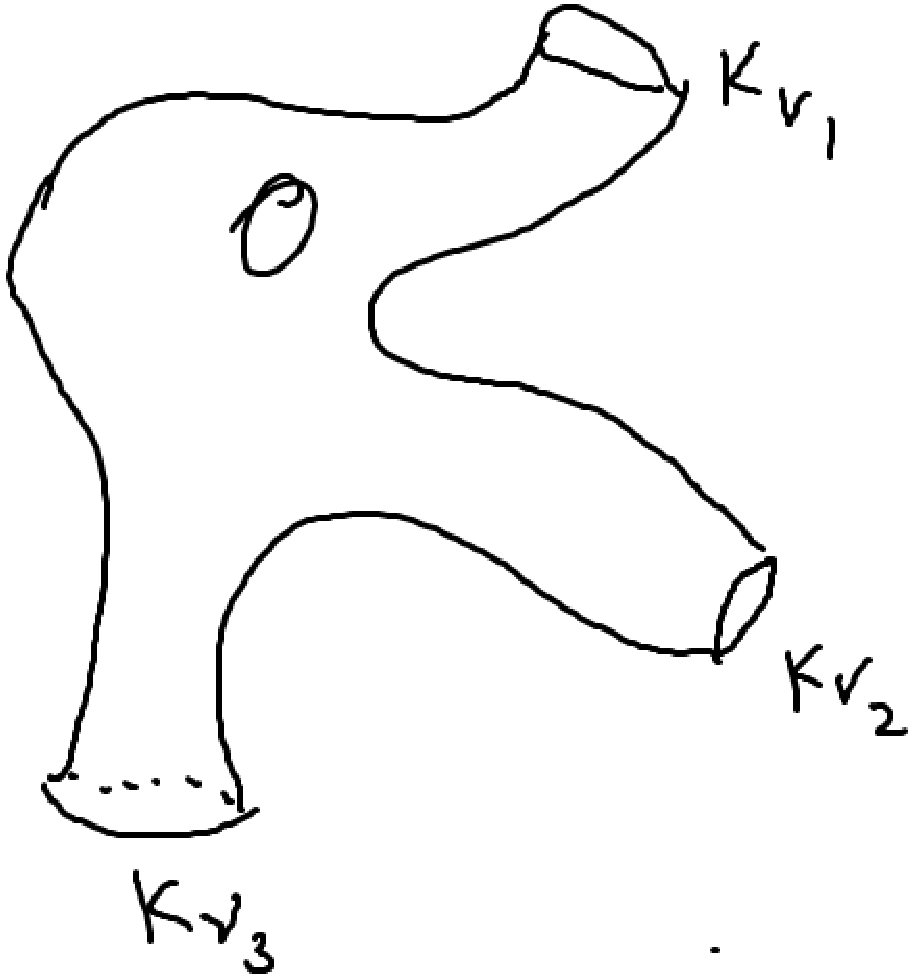
\includegraphics[width=0.30\textwidth]{f21-specO.png}
  \caption{$\Spec\mathcal O$ 类似于一个 3-流形，其边界是 $\bigsqcup_{\nu\in S}\Spec K_\nu$}
  \label{fig:specO}
\end{figure}

当然，作为一个拓扑空间，$\Spec\mathcal O$ 并不是 3 维的。更一般地，我们要强调：本讲义里记录下来的这些几何类比只是类比，我们并不是在把它们当作关于概形或空间的精确事实来陈述。

在 $\mathcal O=\mathbb Z[\frac12]$ 的例子中，$\Spec\mathbb Z[\frac12]$ 有两个边界分支，即 $\Spec\mathbb R$ 与 $\Spec\mathbb Q_2$，见图 \ref{fig:specZ12}。此外，素理想像纽结/循环——图 \ref{fig:knot} 把 $\mathbb Z[\frac12]$ 的素理想 $(3)$ 画成一个纽结/循环。

\begin{figure}[htbp]
  \centering
  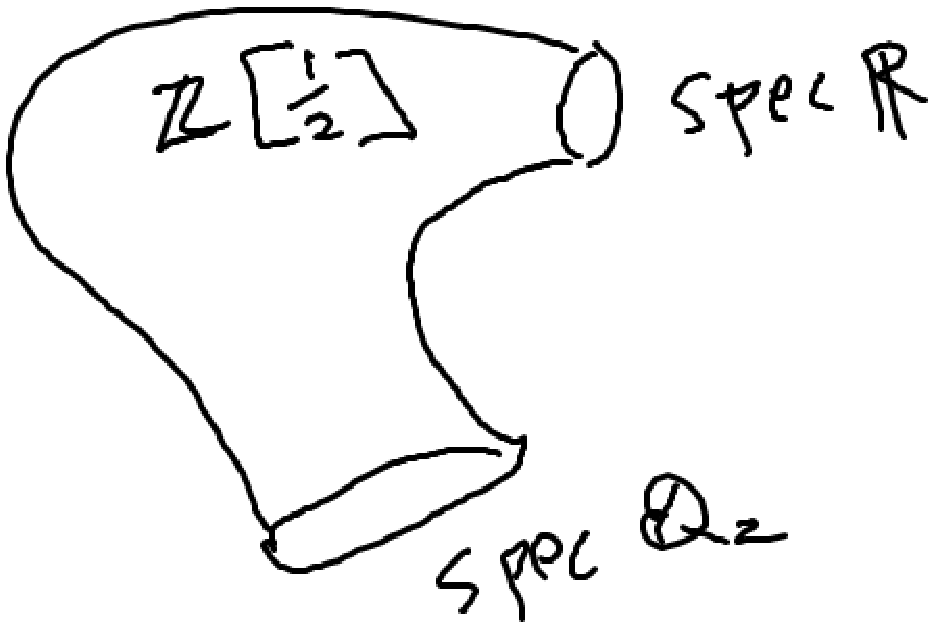
\includegraphics[width=0.30\textwidth]{f22-specZ12.png}
  \caption{$\Spec\mathbb Z[\frac12]$ 类似于一个 3-流形，其边界是 $\Spec\mathbb Q_2\sqcup\Spec\mathbb R$}
  \label{fig:specZ12}
\end{figure}

从 $\Spec\mathbb Z[\frac12]$ 出发，把与素理想 $3\mathbb Z$ 对应的纽结周围的管状邻域挖掉，就得到 $\Spec\mathbb Z[\frac16]$；这里所说的实心管是 $\Spec\mathbb Z_3$，其边界是 $\Spec\mathbb Q_3$，见图 \ref{fig:tube}。换言之，沿 $\Spec\mathbb Q_3$ 把 $\Spec\mathbb Z_3$ 粘到 $\Spec\mathbb Z[\frac16]$ 上，就得到 $\Spec\mathbb Z[\frac12]$。

\begin{figure}[htbp]
  \centering
  \begin{minipage}[t]{0.32\textwidth}
    \centering
    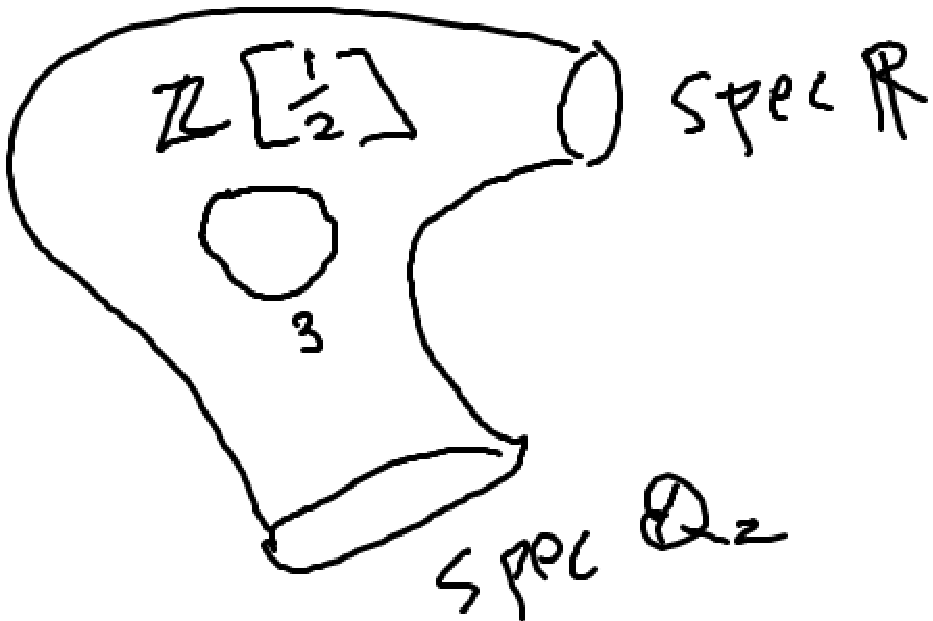
\includegraphics[width=\textwidth]{f23-knot.png}
    \caption{$\Spec\mathbb Z[\frac12]$ 的素理想 $(3)$ 类似于 3-流形中的一个纽结/循环}
    \label{fig:knot}
  \end{minipage}\hfill
  \begin{minipage}[t]{0.32\textwidth}
    \centering
    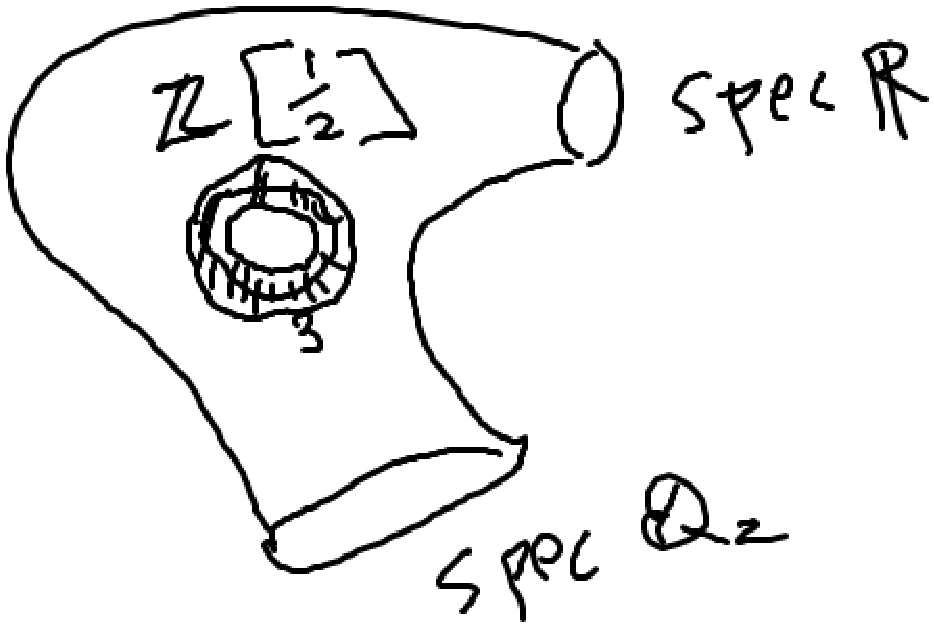
\includegraphics[width=\textwidth]{f24-tube.png}
    \caption{在对应于 $\mathbb Z[\frac12]$ 的素理想 $(3)$ 的纽结周围画出实心管；把这根实心管挖掉就得到 $\mathbb Z[\frac16]$}
    \label{fig:tube}
  \end{minipage}
\end{figure}

\textbf{Langlands 作为 4 维 TQFT}\enspace 字典里没有 4-流形，所以我们从「把向量空间配给类似于 3-流形的算术对象」开始：
\begin{center}
\begin{tabular}{rcl}
「3-流形」 & $\mapsto$ & 向量空间\\
「2-流形」 & $\mapsto$ & 范畴\\
「1-流形」 & $\mapsto$ & 2-范畴
\end{tabular}
\end{center}

例如对 $G=\operatorname{SL}_n$（问题：若 $G$ 不是 $\operatorname{SL}_n$，下面的一切会变吗？），这个「TQFT」$A_G$ 的作用如下：
\[
\begin{array}{r@{\quad}l}
\text{3d} &
\begin{cases}
\mathbb Z\mapsto G(\mathbb Z)\backslash G(\mathbb R)\ \text{上的函数，即自守形式}\\[1pt]
\mathbb Z[\tfrac1p]\mapsto G(\mathbb Z[\tfrac1p])\backslash\bigl(G(\mathbb R)\times G(\mathbb Q_p)\bigr)\ \text{上的函数}\\[1pt]
\mathbb F_p\ \text{上的曲线}\ X\mapsto \Bun_G X\ \text{上的函数}
\end{cases}\\[22pt]
\text{2d} &
\begin{cases}
\mathbb R\ \text{或}\ \mathbb Q_p\mapsto \Rep G(\mathbb R)\ \text{或}\ \Rep G(\mathbb Q_p)\quad\text{（局部 Langlands）}\\[1pt]
\overline{\mathbb F}_p\ \text{上的曲线}\ X\mapsto \Shv(\Bun_G X)\quad\text{（整体几何 Langlands）}
\end{cases}
\end{array}
\]

在配边一侧，$\partial\mathbb Z[\frac1p]=\mathbb R\sqcup\mathbb Q_p$；在代数一侧，
$\{G(\mathbb Z[\frac1p])\backslash(G(\mathbb R)\times G(\mathbb Q_p))\ \text{上的函数}\}\in\Rep\bigl(G(\mathbb R)\times G(\mathbb Q_p)\bigr)$（正则表示）。这与 4 维 TQFT 里带边流形的工作方式一致：带边的 3-流形应当被送到一个范畴连同其中一个对象。

至于复合，由于 $\Spec\mathbb Z[\frac1p]\cup_{\Spec\mathbb Q_p}\Spec\mathbb Z_p=\Spec\mathbb Z$，我们期望
\[
A_G(\mathbb Z)=\Hom_{\Rep G(\mathbb Q_p)}\bigl(A_G(\mathbb Z_p),A_G(\mathbb Z[\tfrac1p])\bigr),
\]
（或者反过来，但那样行不通）。这就迫使 $A_G(\mathbb Z_p)=\operatorname{ind}_{G(\mathbb Z_p)}^{G(\mathbb Q_p)}\mathbf 1$（按定义，$\operatorname{ind}_H^G\rho=\{\phi:G\to V:\phi(gh^{-1})=\rho(h)\phi(g);\ \phi\ \text{模}\ H\ \text{有紧支集}\}$）。

这也说明 $\operatorname{End}_{\Rep G(\mathbb Q_p)}A_G(\mathbb Z_p)$ 作用在 $A_G(\mathbb Z)$ 上（通过复合）。事实上 $\operatorname{End}_{\Rep G(\mathbb Q_p)}A_G(\mathbb Z_p)$ 就是 $G(\mathbb Q_p)$ 的（无分歧）Hecke 代数。因此 $A_G$ 里已经内建了一大堆算子。

\textbf{互反性}\enspace Langlands 纲领的中心猜想之一是「互反」，即一个双射
\[
\{\text{Hecke 算子的特征函数}\}\longleftrightarrow\{\text{同态}\ \pi_1(\text{算术对象})\to\check G\}.
\]
记作 $A_G\xrightarrow{\sim}B_{\check G}$。

$A_G\xrightarrow{\sim}B_{\check G}$ 是上述算术 TQFT $A_G$ 与另一个算术 TQFT $B_{\check G}$ 之间的等价。断言这两个算术 TQFT 等价，就把 Langlands 纲领的各个层次编码在一起——代入数域、局部域等等，就得到相应类型的双射。这种表述的好处，不在于能得到新陈述（因为特化到每个算术对象时，得到的都是已知陈述），而在于它给出一种统一的方式来谈论贯穿 Langlands 纲领的现象，而不必把各种情形分开处理。人们可以在 Langlands 纲领的不同部分还原出许多不同的方面与陈述。相对 Langlands 对偶是类似的现象——它存在于 Langlands 纲领的每一层——因此上述等价是一个有用的方式，用来在头脑中组织并追踪各层之间的关系。

\medskip
\noindent\textbf{练习 1}\enspace
\begin{enumerate}[label=(\alph*),leftmargin=2.0em,itemsep=0.35em,topsep=0.2em]
\item 我们需要验证
\[
\sum_i q^{-\frac i2}\operatorname{tr}\bigl(g\,\big|\,\mathbb C[Y]_i\bigr)=\frac{1}{(1-q^{-\frac12}x)(1-q^{-\frac12}x^{-1})}.
\]
右端是两个几何级数之积。$q^{-\frac i2}$ 的系数是 $x^{-i}+x^{-i+2}+\cdots+x^i$，它应当等于 $\operatorname{tr}\bigl(x\,\big|\,\mathbb C[Y]_i\bigr)$。

$\mathbb C[Y]=\mathbb C[T^*\mathbb A^1]=\mathbb C[q,p]$。对 $f\in\mathbb C[q,p]$，有 $x\cdot f(q,p)=f\bigl((q,p)\cdot x\bigr)=f(xq,x^{-1}p)$；特别地 $x\cdot q=xq$、$x\cdot p=x^{-1}p$。

$\mathbb C[Y]_i$ 的一组基是 $\{q^ip^0,\dots,q^0p^i\}$；在 $x$ 的作用下它变成 $\{x^iq^ip^0,\dots,x^{-i}q^0p^i\}$。因此 $\bigl.x\bigr|_{\mathbb C[Y]_i}$ 是对角矩阵，迹为 $x^i+x^{i-2}+\cdots+x^{-i}$。
\item 等价地，$x\in\mathbb C^*$ 现在对角地作用在 $Y^2$ 上。
\item $\operatorname{Ad}_g\begin{pmatrix}a&b\\c&d\end{pmatrix}=\begin{pmatrix}a&x^2b\\x^{-2}c&d\end{pmatrix}$。因此，等价地，$x^2\in\mathbb C^*$ 作用在 $Y\times Y$ 上，在第一个 $Y$ 上平凡作用，在第二个 $Y$ 上按 (a) 的方式作用。
\end{enumerate}

% !TEX root = ../main.tex
% 第一日第三讲（Yiannis）：相对 Langlands 作为 TQFT
\section{第一日第三讲（Yiannis）}

今天的第一场报告讲的是（4 维）TQFT，第二场讲的是把 Langlands 看作 TQFT。
这第三场讲的是把相对 Langlands 看作 TQFT。
这里，相对 = Langlands + 一些装饰。

先快速回顾前两场讲过的东西。
一切都是 4 维 TQFT：对一个 $d$ 维闭流形 $C$，配上一些态空间 $A_G(C)$，其范畴复杂度与维数相反，即 $A_G(C)$ 是一个 $4-d-1$-范畴，其中 $-1$ 是数、$0$ 是向量空间、$1$ 是范畴。

设 $G$ 是局部域或整体域上分裂的连通约化代数群。
下面是 Langlands 的 A 侧理论的三个典型例子，其中 $G$ 给出与 $C$ 相伴的 A 侧理论 $A_G(C)$。

\begin{exmp}
$C=$ 整体域 $F$，例如数域，或函数域 $\mathbb F_q(\gamma)$，其中 $\gamma$ 是某条光滑射影曲线。
此时 $C$ 是某种 3 维流形。
与之相应的 $A_G(C)$，在 $F$ 为数域时会是一些处处无分歧的自守函数 $\Fns(G(F)\backslash G(\mathbb A_F)/G(\hat O))$。

在函数域情形有两种理解方式。
一种与上面的数域情形相同。
另一种理解是：$\mathbb F_q$ 上曲线 $\gamma$ 的 $G$-丛的群胚的同构类集合。
\end{exmp}

\begin{exmp}
设 $F_v$ 是某个局部域，例如 $F_v=\mathbb Q_p$ 或 $\mathbb F_q((t))$。
它们是 2 维的。
于是我们配给它 $A_G(C)$，即 $G(F_v)$-表示的范畴。
\end{exmp}

\begin{exmp}
2 维的另一个例子是 $\overline{\mathbb F}_q(\gamma)$。
配给它的范畴是 $\Bun^\gamma_G$ 上的层范畴，记作 $\Shv(\Bun^\gamma_G)$。
\end{exmp}

在讨论上述例子的边界条件之前，先回顾前几讲里的一些配边例子。

设 $S$ 是域 $F$ 的一个有限位点集，$\mathcal O_S$ 是 $S$-整数环。
则 $C=\Spec\mathcal O_S$ 是一个带边流形，其边界为 $\bigsqcup_{v\in S}\Spec F_v$。
我们把 $C$ 看作从空集到边界 $\partial C$ 的配边；按 TQFT 的说法，它对应于一个从单位对象到边界上的理论 $A(\partial C)=\Rep G(F_v)$ 的映射。
给出这样的映射，等同于给出 $A(\partial C)$ 中的一个对象；我们取在 $S$ 中各点可能分歧的自守形式，即 $\Fns(G(F)\backslash G(\mathbb A_F)/G(\hat O_S))$。

上述例子展示了第一个例子的理论与第二个例子的理论之间的部分关系，告诉我们它们如何粘在一起。
第一个例子与第三个例子之间也有关系，由某种 Frobenius 迹给出。
下面给出这背后的几何图景。

\inlfig[0.36\textwidth]{f31-mappingcyl}

给定 $\mathbb F_q$ 上的光滑射影曲线 $\gamma$，有映射 $\gamma\to\Spec\mathbb F_q$。
如 David 所解释，$\Spec\mathbb F_q$ 应看作某种圆，因为其平展覆盖的 Galois 群本质上是 $\mathbb Z$。
圆上的一点对应于选取一个代数闭包（非典范的），即一个映射 $\Spec\overline{\mathbb F}_q\to\Spec\mathbb F_q$。
该点上的纤维，就是把曲线 $\gamma$ 基变换到所选代数闭包所得的 $\gamma_{\overline{\mathbb F}_q}$；在几何类比中（把代数闭包换成 $\mathbb C$），它是一个 Riemann 曲面。
一句话，$\gamma$ 应看作圆上的一族 Riemann 曲面。
但这族曲面在拓扑上并不平凡：存在一个 Frobenius 作用，也有 David 在第一讲里解释过的映射柱构造。
Frobenius 作用会告诉你绕圆一周的单值，这就让你把 $\gamma$ 看作某种 3 维的东西，并对该作用取「迹」。
存在一个由 Frobenius 作用给出的范畴迹，把第一个例子的理论与第三个例子的理论联系起来。

那么，什么是相对 Langlands？什么是带边 TQFT？
让我画一幅 David 没时间画的图\zy{原文此处说「让我画一幅 David 没时间画的图」，但 PDF 在这一句与下一页之间没有插入任何图；紧接着的正文又提到「图中右侧的平凡配边」。这里按原文照译，实际图形缺失。[译者按（无外部依据）：依扫描原样报告，未补绘。]}。
他明天会更多地讲这一点。

于是想法是这样的：在 David 的报告里，我们的范畴是某个带配边的流形。
对每个流形，都有一个典范但「无聊」的配边，从该流形到它自身（把流形与区间 $[0,1]$ 相乘）。
这只是恒等映射。
所以带边的理论允许你删掉一些边界，同时仍把它当作你的周期的合法输入。
这意味着，当你把范畴扩大时，可以删掉边界，并把平凡配边（图中右侧）看作从空集到该流形的态射。
每个带边流形都带有从空集出发的典范态射。
因此，无论这里的理论 $A_G(C)$ 是什么（配给流形 $C$ 的），它都会带有从单位元出发的典范映射。
所以新理论（带边的）更丰富：它不只给出某个范畴，还给出该范畴中的一个对象。
当然，这个「杰出元」需要更多数据才能产生，而在我们的理论里，这些数据就是某个带 $G$-作用的空间 $X$。
这个元素将记作 $\mathcal O_{G,X}$。

我想在不谈哈密顿空间与辛空间的前提下，谈论这些额外数据（「装饰」）。
玩具情形的原型是 $G$ 为有限群。
设 $X$ 是带 $G$-作用的向量空间。
此时（回忆 $\mathcal F_G(C)$ 是场论）
\[
  \mathcal F_G(C)=\Maps(C,\mathrm{pt}/G)=\Hom(\pi_1(C),G)/\sim
\]
其中 $\sim$ 是 $G$-共轭。
事实上 $\mathcal F_G(C)$ 有很多名字，如 $\Bun_G$ 与 $\Loc_G$（有限群情形下它们相同）。
与 $C$ 相伴的 A 侧理论是 $A_G(C)=\Fns(\mathcal F_G(C))$。
因此，边界条件应是 $\mathcal F_G(C)$ 上的一个杰出函数，我们把它记作 $\mathcal O_{G,X}$。
记号提示：它由 $G$-空间 $X$ 的额外数据给出。

取主 $G$-丛 $\mathcal E_G\to C$。
由于 $G$ 作用在 $X$ 上，我们可以构造 $C$ 上的一个向量丛，记作 $X\times^G\mathcal E_G$：取 $X$ 与 $\mathcal E_G$ 的积，再模掉对角作用。

于是，在 $\Bun_G=\mathcal F_G(C)$ 上可以构造空间
\[
  \Bun^X_G=\bigl\{(E_G,\sigma):\sigma=\text{section of }X\times^G E_G\bigr\}.
\]
与这组数据相伴的杰出函数 $\mathcal O_{G,X}$ 定义为
\[
  E_G\mapsto\#\{\sigma\}=\#(\Bun^X_G)_{E_G}=\#X^\phi.
\]
最后一个等式来自把 $E_G\in\Maps(C,\mathrm{pt}/G)$ 与单值 $\phi\in\Hom(\pi_1(C),G)/\sim$ 等同起来。
此时 $\#\{\sigma\}$ 不过是 $X$ 在该单值作用下的不动点个数。

然而在 Langlands 的背景下，$\mathcal O_{G,X}$ 的上述两种描述之间有差别，但哲学是一样的。

玩具情形意在让你初步了解空间 $X$ 如何产生边界条件。
其实 $X$ 不必是向量空间，它可以只是一个集合。

现在回到我们的三个例子：在这些情形中 $\mathcal O_{G,X}$ 是什么？
下表是一个总结。

\begin{center}
\scriptsize
\renewcommand{\arraystretch}{1.3}
\begin{tabular}{|p{0.135\textwidth}|p{0.235\textwidth}|p{0.215\textwidth}|p{0.175\textwidth}|}
\hline
 & 例 1 & 例 2 & 例 3\\\hline
$C$\newline[维数 $d$ 的流形]
 & 整体域 $F$，[$d=3$]，\newline 例如数域、函数域 $\mathbb F_q(\gamma)$
 & 局部域 $F_\nu$，[$d=2$]，\newline 例如 $\mathbb Q_p$、$\mathbb F_q((t))$
 & $\overline{\mathbb F}_q(\gamma)$，\newline [$d=2$]\\\hline
$A_G(C)$\newline[$(4-d-1)$-范畴]
 & $\Fns(G(F)\backslash G(\mathbb A_F)/G(\hat O))$，\newline（函数域情形可看作 $\Bun^\gamma_G$）
 & $G(F_\nu)$-表示
 & $\Shv(\Bun^\gamma_G)$\\\hline
$\mathcal O_{G,X}$
 & 周期函数 $\mathcal P_X$
 & $\Fns(X(F_\nu))$
 & 把常值层 $\mathbb C\in\Shv(\Bun^X_G)$ 前推到 $\Shv(\Bun_G)$\\\hline
$B_{\check G}(C)$
 & 落入 $\check G$ 中的 Langlands 参数上的函数
 & 上同调 Langlands 对偶层（局部 Langlands 参数）
 & $\QCoh^!(\Loc^\gamma_{\check G})$\\\hline
$\mathcal O_{\check G,\check X}$
 & 某些 L-函数
 & （将在后续讲义中出现）
 & （将在后续讲义中出现）\\\hline
\end{tabular}
\end{center}

先看第三个例子。
$\mathcal O_{G,X}$ 应当是空间 $\Bun_G=\Bun^\gamma_G$ 上的某个层。
$X$ 的额外数据给出 $\Bun_G$ 上的空间 $\Bun^X_G$。
把常值层前推，就得到 $\Shv(\Bun_G)$ 中的一个元素。

现在来看看另外两个例子中的边界条件是什么。
先想象一下 Frobenius 迹在这里会给出什么。
对第一种情形，我们应当给出某些自守函数。
在函数域情形，它可以看作曲线 $\gamma$ 的 $\Bun_G$ 上的函数。
这种情形下边界条件的函数将称作周期函数，记作 $\mathcal P_X$，即 $\mathcal O_{G,X}=\mathcal P_X$。
这里 $X$ 是 $\mathbb F_q$ 上带 $G$-作用的簇。
函数定义在 $G$-丛上，所以我们把 $G$-丛的记号改为 $[g]$（此前是 $\mathcal E_G$）。
改记号的原因是我们把它们与双商中的阿代尔点等同起来。
现在函数定义为
\[
  \mathcal P_X([g])=\#\{\text{sections of }[g]\times^G X\to\gamma\}
\]
（这个数有限吗？可以是有理数吗？）

而若把 $X$ 的 $\hat O$-点的示性函数记作 $\mathbf 1_X$，周期函数还有另一种写法：
\[
  \mathcal P_X([g])=\sum_{\gamma\in X(F)}\mathbf 1_X(\gamma g)
\]
其中 $F$ 是整体域。

这种自守函数的构造对更一般的一类函数也有效。
对 $X(\mathbb A)$ 上具有所需性质的函数 $\Phi$（比如速降、紧支集、在 $X(\hat O)$ 平移下不变），可以把 $\Phi$ 沿 $X(F)$ 中点的左平移求和。
因为当 $X$ 是仿射簇时 $X(F)$ 是离散集，这个和有定义。
所得函数在左 $G(F)$ 作用下不变，因为集合 $X(F)$ 在 $G(F)$ 下不变。
这类构造一般称作 theta 级数；在具体语境中也可能称作 Poincaré 级数、（伪）Eisenstein 级数等。

最后，第二个例子要给出的边界条件是什么？
我们要放的是某个 $G(F_v)$-表示。
所以它不过是 $X(F_v)$ 上的函数空间。
它是 $G(F_v)$-表示，因为 $G$ 作用在 $X$ 上。

现在花点时间解释 $\Bun^\gamma_G(\mathbb F_q)$ 与阿代尔点 $G(\mathbb F_q)\backslash G(\mathbb A)/G(\hat O)$ 是如何等同的。

给定 $G$-丛 $E$，可以找到曲线 $\gamma$ 的一个开子集 $U$，使 $E$ 限制到 $U$ 上同构于平凡 $G$-丛。
这个同构当然不是给定的，但可以选取。
$U$ 在 $\gamma$ 中的补集是有限个点。
所以要得到 $E$，只需把 $U$ 上的 $G$-丛与每个不在 $U$ 中的点周围形式圆盘上的 $G$-丛粘起来。
这个等同的细节留作练习。

以上所谈的只是 Langlands 的一侧，通常称作理论的 A 侧。
但 Langlands 有两侧，以及两侧之间的对偶。
那么 B 侧是什么？
B 侧应当是与对偶群 $\check G$ 相伴的理论。

回忆第一个例子里，理论的 A 侧只是函数 $\Fns(\Bun_G(F))$。
B 侧理论 $B_{\check G}(C)$ 也是函数，但粗略地说，是到 $\check G$ 中的 Langlands 参数上的函数。
这里的对偶是什么？
对偶是两个函数空间之间的同构，是 Fourier 变换的某种非交换版本。
对自守函数，你应当做谱分解，分解到 Hecke 算子的特征函数上去。
没有 Hecke 算子，一切都没有意义。
这些等价背后隐含地有 Hecke 算子，它们让你能对空间做谱分解，而在 B 侧它们应当是算子的联合特征值。
最非平凡的一点是：A 侧原本没有 Galois 理论，但 Hecke 算子把它与带 Langlands 参数的 B 侧联系起来，而 Langlands 参数与 Galois 表示相关。

在第三个例子里，A 侧理论是 $\Bun_G$ 上的某个层，B 侧理论是某个拟凝聚层 $\QCoh^!(\Loc^\gamma_{\check G})$。
关于它我不打算说什么，只是为了完整而提一句。

第二个例子里的 B 侧理论，对应于 A 侧（即 $G(F_v)$ 的表示），也应当是某种谱分解。
这个范畴 Langlands 对偶最著名的版本是由 Fargues 与 Scholze 证明的。
还有一个由朱歆文证明的版本。

相对 Langlands 对偶应当处理第三列，即边界条件。
对 B 理论也应当有相应的边界条件 $\mathcal O_{\check G,\check X}$。

比如在第一个例子里，边界条件是某些周期函数或 theta 理论，相应的 B 侧边界条件是某个「L-函数」。
我们关于这个对偶所有的证据，要么来自这种情形（我们对周期与 L-函数有所了解），要么来自第二种情形。
但这些我就不讲了。

关于由 $X$ 或 $\check X$ 给出的边界条件，我其实说了点谎。
事实上它们一般与各自余切空间的类比物相关联。
所以猜想的相对 Langlands 对偶，实际上是在 $(G,M)$ 与 $(\check G,\check M)$ 之间，其中 $M,\check M$ 是哈密顿 $G$-空间、$\check G$-空间。
在某些例子里，$M$ 可以解释为余切空间 $T^*X$。

最后给出一个数论的例子，把 theta 级数与周期等同起来；这就是 Tate 论文里的例子。
考虑 $X=\mathbb A^1$，带 $G=\mathbb G_m$ 的作用。
取函数
\[
  \Phi=\Bigl(\bigotimes_{\nu<\infty}\mathbf 1_{\mathbb Z_p}\Bigr)\otimes\Phi_\infty,
  \qquad \Phi_\infty\in\mathcal S(\mathbb R),
\]
其中可取 $\Phi_\infty=e^{-x^2}$（Gauss 函数）。
由这个 $\Phi$ 构造的 theta 级数是
\[
  \sum_{q\in X(\mathbb Q)}\Phi(qg),\qquad g=(1,\cdots,1,x)\in[G].
\]
现在，若一个有理数属于每个 $\mathbb Z_p$，它必须是整数。
于是
\[
  \sum_{q\in X(\mathbb Q)}\Phi(qg)=\sum_{n\in\mathbb Z}\Phi_\infty(nx)
  =\sum_{n\in\mathbb Z}e^{-n^2x^2}.
\]

% !TEX root = ../main.tex
% 第二日第一讲：TQFT 续论、自守理论、Hecke 算子
\section{第二日第一讲}

\subsection{TQFT 续论}
上一次（第一日第一讲）我们讲了 TQFT 的概念，把它当作把到 $BG=\bullet/G$ 的映射线性化的手段。
在第一日第三讲里我们考虑过 $|G|<\infty$ 的例子：一个 TQFT $A_G$ 连同场的数据 $\mathcal F_G$，使得
\[
  \mathcal F_G(C)=\Bun_G(C)=\Maps(C,\bullet/G)=\Hom(\pi_1(C),G)/G.
\]
注意在 $G$ 有限的前提下，$\Loc_G(\Sigma)=\Bun_G(\Sigma)=\Maps(\Sigma,\bullet/G)$，本节里我们随意地这样假定。
例如
\[
  \mathcal F_G(S^1)=\Maps(S^1,\bullet/G)=\Hom(\mathbb Z,G)/G=G/G,
\]
其中商是对共轭作用取的。

我们也可以把 $\bullet/G$ 换成一个有限群胚（栈）$X=X/G$，其中 $X$ 是 $G$-空间，并取 $\mathcal F_G$ 为
\[
  \mathcal F_G(S^1)=\Loc^X_G(S^1)=\Bun^X_G(S^1)=\Maps(S^1,X/G)
  =\{x\in X,\ g\in G,\ g\cdot x=x\}/G
\]
（把 $S^1$ 换成一般的 $\Sigma$ 也类似）。

注意有一个由 $X/G\to\bullet/G$ 诱导的映射 $\Loc^X_G(\Sigma)\to\Loc_G(\Sigma)$，因为 $\Loc_G(\Sigma)=\Maps(\Sigma,\bullet/G)\,(=\Bun_G(\Sigma))$。
一旦固定了这样的 $G$-空间 $X$，我们就有一个杰出元
\[
  \Theta_{G,X}(\Sigma)\in Z^3_G(\Sigma)=\mathbb C[\Loc_G(\Sigma)],
\]
它定义一个边界理论 $\Theta_{G,X}$。

4 维（算术）TQFT $Z=A_G$ 可以通过先取场 $\mathcal F_G=\Bun_G(-)=\Maps(-,\bullet/G)$、再线性化（取空间上的函数/层）得到，其抽象说法如下图所示：
\[
\begin{array}{ccc}
\text{流形}/\!\!\text{ 配边} & \xrightarrow{\quad A_G\quad} & \text{线性范畴}/\!\!\text{ 态射}\\[2pt]
\searrow^{\ \mathcal F_G} & & \nearrow_{\ \text{取函数/层}}\\[2pt]
& \text{群胚（栈）}/\!\!\text{ 对应} &
\end{array}
\]

我们来讨论 $A_G$ 的函子性。
我们知道 $A_G$ 经 $\mathcal F_G$ 因子化，所以先描述 $\mathcal F_G$ 的函子性。
给定配边
\[
  M:\partial_{\mathrm{in}}\to\partial_{\mathrm{out}},
\]
由下面的图得到一种对应
\[
\begin{array}{ccc}
& \mathcal F_G(M)=\Bun_G(M) &\\[2pt]
\swarrow_{\ f} & & \searrow^{\ g}\\[2pt]
\mathcal F_G(\partial_{\mathrm{in}})=\Bun_G(\partial_{\mathrm{in}}) & &
\mathcal F_G(\partial_{\mathrm{out}})=\Bun_G(\partial_{\mathrm{out}}).
\end{array}
\]
然后，沿第一个映射 $f$ 拉回、沿第二个映射 $g$ 前推，就得到态射 $A_G(M):A_G(\partial_{\mathrm{in}})\to A_G(\partial_{\mathrm{out}})$。

此外，给定 $G$-空间 $X$ 时，我们可以定义杰出对象 $\Theta_{G,X}(\Sigma)\in A_G(\Sigma)$。
取一个扩张配边 $M:\emptyset\to\Sigma$（图 4.1）即可得。

\insfig[0.30\textwidth]{f41-empty}{$M:\emptyset\to\Sigma$}

它给出对应
\[
\begin{array}{ccc}
& \Bun^X_G(\Sigma)=\Maps(\Sigma,X/G) &\\[2pt]
\swarrow & & \searrow\\[2pt]
\mathcal F_G(\emptyset)=\bullet & & \mathcal F_G(\Sigma)=\Maps(\Sigma,\bullet/G),
\end{array}
\]
进而给出一个态射 $1\to A_G(\Sigma)$，等价地说，给出 $A_G(\Sigma)$ 中的一个对象 $\Theta_{G,X}(\Sigma)$。
我们就是这样得到周期函数/周期层的（在 B 侧（谱侧）类似地得到 L-函数/L-层）。

\subsection{自守理论}
现在考虑 $G$ 是域 $k$ 上的约化群的情形，得到推广到算术流形的 4 维 TQFT $A_G$。
$A_G$ 由代数 $G$-丛的模空间的拓扑构成。

在整体几何设定中：$\Sigma$ 是 $F=\overline F$（例如 $\mathbb C$、$\overline{\mathbb F}_q$）上的代数曲线（2 维），于是得到 $\mathcal F_{A_G}(\Sigma)=\Bun_G(\Sigma)$。

\begin{exmp}
$\mathcal F_{\mathbb G_m}(\Sigma)=\Pic(\Sigma)$。
\end{exmp}

\begin{exmp}
若 $\Sigma=D^\times_F=\Spec(F((t)))$，则
\[
  \mathcal F_G(D^\times_F)=\Bun_G(D^\times_F)=\bullet/G(F((t))).
\]
\end{exmp}

\begin{exmp}
若 $\Xi$ 是 $\mathbb F_q$ 上的曲线，则
\[
  \mathcal F_G(\Xi)=\Bun_G(\Sigma)^{\Frob}=\Bun_G(\Sigma)(\mathbb F_q).
\]
（这里 $\Sigma$ 是 $\Xi$ 基变换到 $\overline{\mathbb F}_q$ 所得，$\Bun_G(\Sigma)^{\Frob}$ 是关于 Frobenius 的不动点空间。）
\end{exmp}

\begin{exmp}
特别地，若 $\Sigma=D^\times_{\mathbb F_q}=\Spec(\mathbb F_q((t)))$，则
\[
  \mathcal F_G(D^\times_{\mathbb F_q})=\Bun_G\bigl(D^\times_{\mathbb F_q}\bigr)^{\Frob}
  =G(\mathbb F_q((t)))/^{\Frob}G(\mathbb F_q((t)))\supset\bullet/G(\mathbb F_q((t))).
\]
\end{exmp}

现在我们要把上述空间线性化。
注意 $A_G$ 把 3 维流形送到向量空间，把 2 维流形送到线性范畴。

\begin{exmp}
对例 4.3 中的 3 维流形 $\Xi$，有
\[
  A_G(\Xi)=\Fun(\Bun_G(\Sigma)(\mathbb F_q)),
\]
即无分歧自守形式的向量空间。
\end{exmp}

\begin{exmp}
对例 4.4 中的 2 维流形 $D^\times_{\mathbb F_q}$，有
\[
  A_G(D^\times_{\mathbb F_q})=\Shv(\Bun_G(D^\times_{\mathbb F_q}))
  =\Shv\bigl(G(\mathbb F_q((t)))/^{\Frob}G(\mathbb F_q((t)))\bigr),
\]
即与穿孔圆盘相伴的自守范畴；它包含 $\Shv(\bullet/G(\mathbb F_q((t))))=\Rep^{\mathrm{smooth}}(G(\mathbb F_q((t))))$，即该局部域 $\mathbb F_q((t))$ 上的群的平滑表示范畴，也就是经典局部 Langlands 所研究的对象。
\end{exmp}

\begin{exmp}
人们可能以为 TQFT 只编码无分歧部分的信息，但其实它也能看见分歧部分：

\inlfig[0.86\textwidth]{f44-ramified}

我们有 $\Spec(\mathbb Z[1/2])$，把它看作以 $\Spec(\mathbb Q_2)$ 与 $\Spec(\mathbb R)$ 为两个边界分支的 3 维流形。
类似地，可以取有限域 $\mathbb F_q$ 上的曲线 $\Sigma$，挖掉几个点 $x_1,x_2$，然后看 $\Fun(\Bun_G(\Xi|x_1,x_2))$（$\Bun_G$ 上带两个点处某些额外数据的函数）。
这给出 $\Rep G(\mathbb F_q((t)))^2$ 中的一个对象。
细节从略，要点是：TQFT 当然知道如何处理分歧——我们只需挖掉一些东西，于是与闭 3 维流形得到向量空间不同，我们得到与边界相伴的范畴中的一个对象，此地即 $\Rep G(\mathbb F_q((t)))^2$。
\end{exmp}

下图这个菱形给出各种整体/局部、算术/几何设定的大图景：
\begin{center}
\begin{tikzpicture}[scale=0.78, every node/.style={font=\footnotesize}]
  \coordinate (T) at (0,2);
  \coordinate (L) at (-2.9,0);
  \coordinate (R) at (2.9,0);
  \coordinate (B) at (0,-2);
  \draw (T)--(L)--(B)--(R)--(T);
  \node[above] at (T) {$\mathbb Q,\ \Xi=\Sigma$（$\mathbb F_q$ 上）};
  \node[left]  at (L) {$\mathbb Q_p,\ \mathbb F_q((t))$};
  \node[right] at (R) {$\Sigma$（$\mathbb C$、$\overline{\mathbb F}_q$ 上）};
  \node[below] at (B) {$\overline{\mathbb F}_q((t)),\ \mathbb C((t))$};
  \node at (-1.75,1.5) {算术};
  \node at (1.75,1.5)  {整体};
  \node at (-1.75,-1.5) {局部};
  \node at (1.75,-1.5)  {几何};
  \node[right] at (7.0,2)  {3-流形};
  \node[right] at (7.0,0)  {2-流形};
  \node[right] at (7.0,-2) {1-流形};
\end{tikzpicture}
\end{center}

\begin{figure}[htbp]
\centering
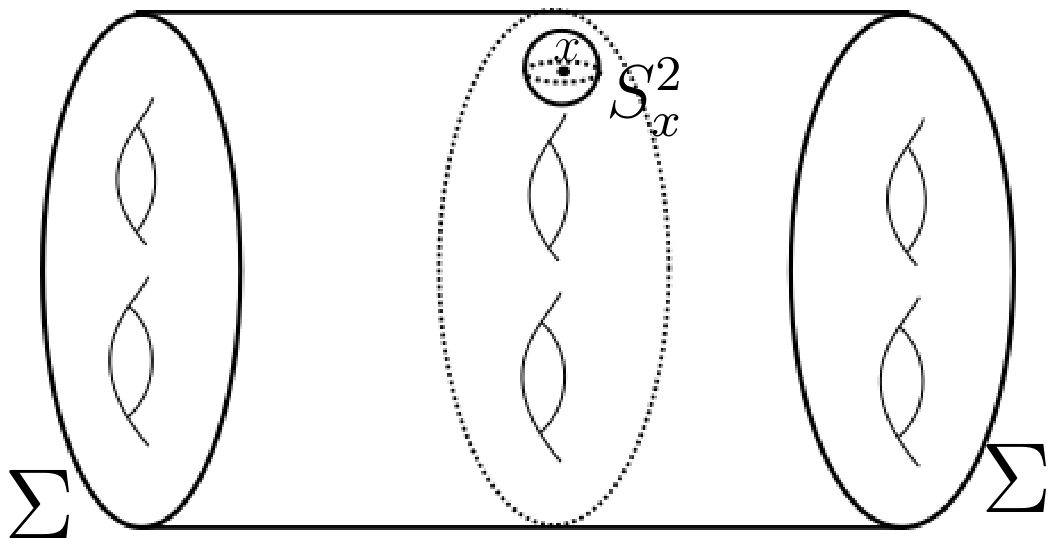
\includegraphics[width=0.72\textwidth]{f42-bordism}
\caption{配边 $(\Sigma\times I)\setminus D^3_x:S^2_x\sqcup\Sigma\to\Sigma$}
\label{fig:f42}
\end{figure}

我们还没有明确所用的层论是什么。
例如，对整体几何 Langlands，有
\[
  A_G(\Sigma)=\Shv^?_N(\Bun_G(\Sigma)),\qquad
  ?=\begin{cases}
    \mathrm{dR}\ (\text{de Rham}), & \text{D-模},\\
    \mathrm{B}\ (\text{Betti}), & \text{向量空间层},\\
    \text{ét}\ (\text{étale}), & \text{平展可构造层}.
  \end{cases}
\]
（确切地说，还需要一处技术性修正才能让一切成立：我们需要取具有幂零支撑的层。
例如当 $G=\mathbb G_m$ 时 $\Bun_G(-)=\Pic(-)$，「幂零支撑」这个形容词让我们只需处理 $\Pic$ 上的局部常值层，而不是所有层。）

\subsection{可观测量的对称性、Hecke 算子}
让我们回到有限群的设定。
设 $H$ 是有限群，于是 $\Bun_H(-)=\Loc_H(-)$。
考虑昨天讲过的与有限群 $H$ 相伴的 4 维 TQFT $Z^4_H$，使得 $Z^4_H(\Sigma)=\Vect(\Bun_H(\Sigma))$。
这个范畴有很好的对称性，并且被可观测量作用，即被 $Z^4_H(S^2)$（又称 Hecke 范畴/线算子范畴）作用，如昨天第一讲所解释。
这个作用可以通过把 $Z^4_H$ 作用于图 4.2 中的配边（选好 $x\in\Sigma$）得到：

具体地，
\[
  Z^4_H(S^2_x)=\Vect(\bullet/H)=(\Rep(H),\otimes)
\]
（因为 $\Bun_H(S^2)=\Loc_H(S^2)=\bullet/H$），它如下作用于 $Z^4_H(\Sigma)$：
\begin{itemize}[leftmargin=2.0em,itemsep=0.3em]
\item 对每个 $x\in\Sigma$，有映射
\[
  \Bun_H(\Sigma)\xrightarrow{\ (-)|_x\ }\Bun_H(x)=\bullet/H;
\]
\item 给定 $V\in Z^4_H(S^2)=\Rep(H)$，沿上述映射把它拉回，得到 $\Bun_H(\Sigma)$ 上的向量丛 $V_x$。
\end{itemize}

\begin{figure}[htbp]
\centering
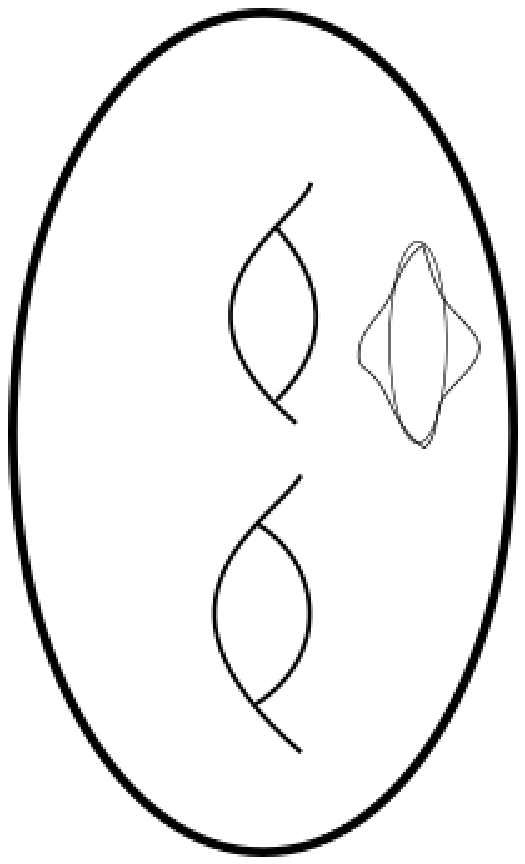
\includegraphics[width=0.24\textwidth]{f43-raviolo}
\caption{$\Sigma\sqcup_{\Sigma\setminus\{x\}}\Sigma
=\Sigma\sqcup_{D_x}\bigl(\text{raviolo}\bigr)
=\Sigma\sqcup_{D_x}\bigl(D_x\sqcup_{D^\times_x}D_x\bigr):\Sigma\to\Sigma$}
\label{fig:f43}
\end{figure}

\begin{itemize}[leftmargin=2.0em,itemsep=0.3em]
\item 于是 $V$ 通过下式作用于 $E\in Z^4_H(\Sigma)$：
\[
  V\cdot E:=V_x\otimes E.
\]
\end{itemize}

我们在 Langlands 对应的 B 侧（谱侧）将要看到的算子，正是这个样子的。

现在回到 $G$ 是约化群的情形。
取
\[
  Z(-)=A_G(-)=\Shv^?_N(\Bun_G(-))
\]
（或者可以取与圆的乘积再取 Frobenius 的迹；对有限域上的曲线，我们把层换成自守函数）。

要得到 Hecke 算子，我们再次取 $x\in\Sigma$，并看配边（图 4.2）。
取场空间之后，这本应给出一个对应，再线性化就得到 Hecke 作用。
但当然，由于技术上的困难我们不能直接这样做：$I=[0,1]$ 不是代数曲线，所以必须弄清如何在代数几何中解读这一点。
既然一切都应当是局部常值的，可以想象把这张图收缩，得到某个像「$\Sigma$ 沿 $x$ 处的圆盘与一个 raviolo 粘起来」的东西（见下图 4.3）。
raviolo 应看作 $D\sqcup_{D^\times}D$，是扮演 2-球面角色的代数几何对象。

取场空间之后就得到对应，即 Hecke 对应：
\[
\begin{array}{ccc}
& \Bun_G(\Sigma\sqcup_{\Sigma\setminus\{x\}}\Sigma)=\mathrm{Hecke}_x &\\[2pt]
\swarrow & & \searrow\\[2pt]
\Bun_G(\Sigma) & & \Bun_G(\Sigma).
\end{array}
\]
这里 $\Bun_G(\Sigma\sqcup_{\Sigma\setminus\{x\}}\Sigma)$ 的元素，无非是在 $x$ 之外等同起来的一对 $G$-丛，但也可以看作 $\Sigma$ 上的单个 $G$-丛连同 $x$ 处局部修改的某些局部数据。
现在取自守函数/层，沿第一个映射拉回、乘/张量上 $A_G(\text{raviolo})$ 中的某个东西、再沿第二个映射前推，就得到算子/函子。
这就给出 $A_G(\text{raviolo})$ 在 $A_G(\Sigma)$ 上的 Hecke 作用。

\begin{exmp}
\leavevmode\par
\begin{itemize}[leftmargin=2.0em,itemsep=0.3em]
\item （算术设定，来自第一日第二讲）回忆在算术语境中，Hecke 算子的作用是这样得到的：取与数域相伴的对象，挖掉一个素点（即把该素点反转），再把它粘回去，于是得到粘回去的那个东西的自同态。
该设定中的 Hecke 作用可以看作恰好来自上面的配边。
\item 若 $G=\mathbb G_m$，则 $\Bun_G(D_x\sqcup_{D^\times_x}D_x=:\text{raviolo})=\mathbb C((t))^\times/\mathbb C[[t]]^\times\cong\mathbb Z$，而 $A_G(\text{raviolo})=\Shv(\mathbb Z)$ 在 $A_G(\Sigma)=\Shv(\Pic(\Sigma))$ 上的 Hecke 作用，本质上由 $\mathbb Z$ 在 $\Pic(\Sigma)$ 上的作用 $n:L\mapsto L(nx)$ 诱导。
\end{itemize}
\end{exmp}

\section{第二日第二讲}

\subsection{一个奇迹}

我们从 Riemann zeta 函数讲起，包括对全体整数 $\mathbb Z$ 的求和。某些书里会改用另一个变量 $y=x^2$ 来写下面的公式。

Riemann 证明了
\begin{equation}
  \int_0^\infty x^s\sum_{n\in\mathbb Z}e^{-\pi n^2x^2}\,d^\times x=2\pi^{-s/2}\Gamma(s/2)\zeta(s)=L(\chi,0)
  \label{eq:5-1}
\end{equation}
% [Tutor Note: 原文右端写作 $L(\chi,0)$。按上下文 $\chi:x\mapsto|x|^s$ 应是 $L(\chi,s)$，此处原文疑似笔误，译文照原文保留，已在 reports/ch05.md 登记。]
其中
\begin{equation}
  \chi:\ x\mapsto|x|^s,
  \label{eq:5-2}
\end{equation}
\begin{equation}
  \zeta(s)=\prod_p\frac{1}{1-p^{-s}},
  \label{eq:5-3}
\end{equation}
\begin{equation}
  \sum_{n\in\mathbb Z}e^{-\pi n^2x^2}=\Theta(x),
  \label{eq:5-4}
\end{equation}
即 Jacobi theta 函数，并记
\begin{equation}
  \zeta_\infty(s)=\pi^{-s/2}\Gamma(s/2).
  \label{eq:5-5}
\end{equation}
另外，只是作为一个记号，$d^\times x=\frac{dx}{x}$。

上式是 theta 级数的 Mellin 变换——把它理解为乘法 Fourier 变换。

注意对 theta 函数，在 Poisson 求和公式下有
\begin{equation}
  \theta(x)\ \overset{\text{PSF}}{\longleftrightarrow}\ x^{-1}\theta(x^{-1}),
  \label{eq:5-6}
\end{equation}
类似地
\begin{equation}
  \zeta_\infty(s)\longleftrightarrow\zeta(1-s).
  \label{eq:5-7}
\end{equation}
注意这是周期函数的一例，记作 $P_X$，其中 $X=\mathbb A^1$ 带 $G=\mathbb G_m$ 作用。

注意，把 L-函数写成周期，并没有普遍的理论。在代数几何里，我们有
\begin{equation}
  \text{``Schur Variety''}\ \overset{\text{周期}}{\cong}\ \text{``Schur variety''}.
  \label{eq:5-8}
\end{equation}
% [Tutor Note: 原文左右两侧引号内的写法只差 Variety/variety 的大小写，疑为原文笔误或打字噪声；译文照原文保留大小写差别。]

对阿代尔情形，(5.1) 推广为
\begin{equation}
  \int_{[G_m]}|x|^s\sum_{\gamma\in F=\mathbb A^1(F)}\Phi(\gamma x)\,d^\times x
  \label{eq:5-9}
\end{equation}
这里的积分区域是
\begin{equation}
  [G_m]=G(F)\backslash G(\mathbb A)\quad\text{或}\quad G(F)\backslash G(\mathbb A)/G(O).
  \label{eq:5-10}
\end{equation}
\begin{equation}
  P_X(x)\ \sum_{\gamma\in F=\mathbb A^1(F)}\Phi(\gamma x)\in S(X(\mathbb A))
  \label{eq:5-11}
\end{equation}
% [Tutor Note: 原文此式左端 $P_X(x)$ 与求和号之间没有等号，译文照原文保留。]
是周期，其中 $S(X(\mathbb A))$ 表示 Schwartz 函数，$X$ 是局部的，而
\begin{equation}
  \Phi(\gamma x)=\prod_{p<\infty}\mathbf 1_{\mathbb Z_p}\otimes e^{-\pi x^2_\infty},
  \label{eq:5-12}
\end{equation}
其中 $\mathbf 1_{\mathbb Z_p}$ 带 $G(\hat{\mathbb Z})$ 的单位作用。

这里我们用 idele 类特征
\begin{equation}
  F^\times\backslash\mathbb A^\times\to\mathbb C^\times.
  \label{eq:5-13}
\end{equation}
下面给几条注解。

\begin{enumerate}[label=(\arabic*),leftmargin=2.0em,itemsep=0.25em]
  \item 上述两者的不同在于：一个是自守形式，一个是自守函数。
  \item 可以把上述看作一个带两条边界的 TQFT：一条带 $G(\mathbb R)$ 作用，一条带 $G(\mathbb Q_p)$ 作用。
  \item 当 $X$ 在 $O_v$ 上光滑仿射时，$\mathbf 1_{X(O_v)}$ 是基本函数。
  \item 这个积分是下述构造的特例
  \begin{equation}
    \langle\text{自守形式},\text{周期}\rangle=\text{L-函数}
    \label{eq:5-14}
  \end{equation}
  \item 5.6 可以看作在 $T^*\mathbb A^1=M$ 的两个子空间之间作对换。也就是说，在 PSF 下，
  \begin{equation}
    \mathbb A^1\longleftrightarrow O(\mathbb A^1)^*
    \label{eq:5-15}
  \end{equation}
  在 $T^*\mathbb A^1$ 里是不变的。这里 $M$ 是一个 Hamilton $G$-空间。
\end{enumerate}

现在可以回答这个问题：Riemann 的构造为什么奏效？把 Tate 积分展开（忽略 $\gamma=0$），得
\begin{equation}
  \int_{\mathbb A^1}|x|^s\Phi(\gamma x)\,d^\times x=\prod_{p\le\infty}\int_{\mathbb Q_p^\times}\Phi_p(x)\,d^\times x.
  \label{eq:5-16}
\end{equation}
固定 $p<\infty$，我们有
\begin{equation}
  \int_{\mathbb Z=\mathbb Q_p^\times/\mathbb Z_p^\times}|x|^s\mathbf 1_{\mathbb Z_p^\times}(x)\,d^\times x=\sum_{i\ge0}p^{-is}=\frac{1}{1-p^{-s}}=\zeta_p(s).
  \label{eq:5-17}
\end{equation}
这就是一个奇迹！！！另外，这里 $i=0$ 这一项为 $1$。

\subsection{基本函数的 Mellin 变换}

设 $N:=S(\mathbb Q_p)^{\mathbb Z_p^\times}$。它是 Hecke 代数
\[
  H(\mathbb Q_p^\times,\mathbb Z_p^\times)=\mathbb C[\mathbb Q_p^\times/\mathbb Z_p^\times]=\mathbb C[\mathbb Z]
\]
的模。设 $\mathbf 1_{\mathbb Z_p}\in N$ 是 $\mathbb Z_p$ 上的常函数。

$\zeta_p(s)$ 会出现在 $N$ 的模结构里吗？答案是不会。$N$ 是由 $\mathbf 1_{\mathbb Z_p}$ 生成的秩 $1$ 自由 $\mathbb Z$-模，但考虑
\[
  N^*:=S(\mathbb Q_p^\times)^{\mathbb Z_p^\times}=\mathbb C[\mathbb Z],
\]
它包含元素 $\mathbf 1_{\mathbb Z_p^\times}$，也带 $H(\mathbb Q_p^\times,\mathbb Z_p^\times)$ 的作用，而 $\mathbf 1_{\mathbb Z_p^\times}$ 的 Mellin 变换是 $1$ 而不是 $\zeta_p(s)$。

只有把这个模看作内积空间时，$\zeta$ 才开始出现。内积 $\langle\ ,\ \rangle$ 来自嵌入 $N\hookrightarrow L^2(\mathbb Q_p)$，也就是 $L^2(\mathbb Q_p^\times)$。

澄清一个吹毛求疵的点：做积分时，我们其实考虑的是 $\mathbf 1_{\mathbb Z_p}(x)|dx|^{1/2}$，其中 $|dx|^{1/2}$ 称为半密度。

\subsection{Plancherel 公式}

我们想要形如
\begin{equation}
  \langle f_1,f_2\rangle=\langle\hat f_1,\hat f_2\rangle
  \label{eq:5-18}
\end{equation}
的公式，其中 $\hat f$ 是 $f$ 的 Mellin 变换。函数定义在 $\mathbb Q_p^\times/\mathbb Z_p^\times\equiv\mathbb Z$ 上，所以它们的 Mellin 变换定义在 $\mathbb Z$ 的对偶上；这个对偶是 $S^1\subset\mathbb C$，即酉特征标群。

可以算出
\[
  \widehat{\mathbf 1_{\mathbb Z_p}|dx|^{1/2}}(z)=\frac{1}{1-p^{-1/2}z}\,|d^\times z|^{1/2},
\]
这里 $z\in S^1$ 对应于此前的 $p^{-s}$，而 $p^{-1/2}$ 的移位源于半密度 $|dx|^{1/2}$。

此时公式 (5.18) 读作
\[
  \begin{aligned}
  &\langle\mathbf 1_{\mathbb Z_p}|dx|^{1/2},\mathbf 1_{\mathbb Z_p}|dx|^{1/2}\rangle\\
  &\qquad=\int_{S^1}\frac{1}{(1-p^{-1/2}z)(1-p^{-1/2}z^{-1})}\,d^\times z.
  \end{aligned}
\]
也可以用 Hecke 代数的作用来做。取 $h\in H=\mathbb C[\mathbb Z]$，$h$ 作用在第一项上会在右端把被积函数乘以 $\hat h$。即
\[
  \begin{aligned}
  &\langle h\cdot\mathbf 1_{\mathbb Z_p}|dx|^{1/2},\mathbf 1_{\mathbb Z_p}|dx|^{1/2}\rangle\\
  &\qquad=\int_{S^1}\frac{\hat h(z)}{(1-p^{-1/2}z)(1-p^{-1/2}z^{-1})}\,d^\times z\\
  &\qquad=\int_{S^1}\hat h(z)\zeta_p(\tfrac12+s)\zeta_p(\tfrac12-s)\,d^\times z.
  \end{aligned}
\]

这里藏着对偶的 $\mathbb G_m$，即原 $\mathbb G_m$ 的 Langlands 对偶，以及对偶 $T^*\mathbb A^1=:\check M$。等我们为 L-函数建立一般的形式化时，我们会说这里的 zeta 函数与这个对偶 $\mathbb G_m$ 在同一空间上的作用相关联——这纯属巧合。但这只是对偶性一个非常特殊的例子。

\subsection{Satake 同构}

现在回顾经典 Satake 同构。

设 $H_G=H(G(F),G(O))$ 是 $F$ 上连通分裂约化群概形 $G$ 的球 Hecke 代数。

经典 Satake 同构断言 $H_G\simeq H_T^W$，其中 $T=B/N$。由于下面这族同构，它也等价于 $H_G\simeq\mathbb C[\Rep\check G]$：
\begin{equation}
  H_G\simeq H_T^W=\mathbb C[X_\bullet(T)]^W=\mathbb C[\check T]^W=\mathbb C[\check G]^{\check G}\simeq\mathbb C[\Rep\check G].
  \label{eq:5-19}
\end{equation}
后一个同构 $\mathbb C[\check G]^{\check G}\simeq\mathbb C[\Rep\check G]$ 由特征标映射给出，即从 $\Rep\check G$ 的 Grothendieck 群到 $\check G$ 在自身上伴随作用的不变环的映射。

Hecke 同构的构造这里不回顾，我们只想指出：它用到 $H_G\otimes H_T$-双模 $S(N(F)\backslash G(F))^{G(O)}$。

也可以说，整个图景只有在几何 Satake 等价之后才完全说得通：它把 $H_G$ 变成半单范畴，并断言它等价于 $\Rep\check G$。

此外，经典 Satake 同构从分析的角度看并不很好用。为了看清楚，我们比较两侧的内积。

在右端我们有典范基 $\{s_\lambda\}$，即最低权 $\lambda$ 的不可约表示 $\{V_\lambda\}$ 的 Weyl 特征标；这里 $\lambda$ 取 $T$ 的反支配余特征标（必须取最低权 $\lambda\in X^-_\bullet(T)$，才能使下面的公式成立）。

同时，左端有一个内积，来自嵌入 $H_G\hookrightarrow L^2(G)$。

自然要问：右端的典范基是否对应左端的标准正交基？答案是否。

记 $\hat h$ 为 $h\in H_G$ 在 Satake 同构下的像，并定义 $h_\lambda$ 为满足 $\hat h_\lambda=s_\lambda$ 的元素。

左端当然有一组正交基，由同一集合 $\{\lambda\in X^-_\bullet(T)\}$ 自然地参数化：只需取双 $G(O)$-陪集的示性函数 $\mathbf 1_{G(O)\omega_\lambda G(O)}$。但这并不是我们要找的那组基：$h_\lambda\neq\mathbf 1_{G(O)\omega_\lambda G(O)}$，而且 $\{h_\lambda\}$ 关于来自 $H_G\hookrightarrow L^2(G)$ 的内积并不正交。

于是得到下面的问题：$H_G$ 上使 $h_\lambda$ 正交的自然内积是什么？

为回答它，先回忆 $s_\lambda$ 的正交性是什么意思：可以把 $\{s_\lambda\}$ 看作极大紧子群 $\check G_c\subset G$ 的特征标，于是有
\[
  \int_{\check G_c}s_\lambda\overline{s_\mu}=\delta_{\lambda\mu}.
\]
用 Weyl 积分公式可改写为
\begin{equation}
  \frac{1}{|W|}\int_{\check T_c}s_\lambda(t)\overline{s_\mu(t)}\,d_{Weyl}(t)
  =\int_{\check G_c}s_\lambda\overline{s_\mu}=\delta_{\lambda\mu},
  \label{eq:5-20}
\end{equation}
其中 $d_{Weyl}(t)=\prod_{\check\alpha\in R(\check G)}(1-e^\lambda)$ 是来自 Weyl 特征标公式的 Weyl 测度（这里 $e^\lambda:T\to\mathbb C^\times$ 是由 $\lambda\in X^\bullet(T)$ 给出的映射）。
% [Tutor Note: 原文乘积的指标是 $\check\alpha$，但因子里却写 $e^\lambda$；按 Weyl 特征标公式应是 $\prod_{\check\alpha}(1-e^{\check\alpha})$。译文照原文保留。]

我们要用这个 Weyl 测度在 $G$ 上造一个使 $h_\lambda$ 正交的内积。上面的讨论表明，需要对它作某种非平凡的修正才行。结果表明，正确的修正由群 $G$ 上的 Macdonald 公式提供：我们可以定义
\begin{equation}
  \langle h,\mathbf 1_{G(O)}\rangle=\langle h*\mathbf 1_{G(O)},\mathbf 1_{G(O)}\rangle
  =\frac{1}{|W|}\int_{T_{\check G}}\frac{\hat h(t)}{\prod_{\check\alpha\in R(\check G)}(1-q^{-\frac12}e^{\check\alpha})}\,d_{Weyl}(t).
  \label{eq:5-21}
\end{equation}
右端的修正测度就是该群的 Plancherel 测度。

修正因子可以用 $\check G$ 在其 Lie 代数上伴随表示的 $q$-特征标重写。对此的概念性解释由导出 Satake 同构提供。

\section{第二日第三讲}

设 $F$ 是局部域 $\mathbb Q_p$、$\mathbb F_p((t))$（它们是 $2$ 维的），或者几何局部域 $\mathbb F_p((t))$（它是 $1$ 维的）。设 $O$ 是它的整数环。设 $X$ 是 $G$-簇，从而我们可以把 $X$ 看作带群 $G$ 作用的向量空间。$A_G(F)$ 是 $G(F)$-表示构成的范畴。$\Theta_X\in A_G(F)$ 是 $X(F)$ 上的函数。相对 Langlands 对应给出一个 $\check G$-簇 $\check X$ 以及 $\Theta_{\check X}\in B_{\check G}(F)$。我们想把 $\Theta_X$ 理解成一个 $G(F)$-表示，使得它在 Langlands 对应的 B 侧可以互通。

目前我们的目标是理解无分歧部分：Hecke 代数 $H:=\Hecke(G(F),G(O))$ 作用在 $X(F)$ 的 $G(O)$-不变函数上。我们想把这一作用对角化，并且要求它与来自 $X$ 的额外结构相容。先看一个模型例。

\medskip
\noindent\textbf{例 1（模型例）}\enspace
在 A 侧，我们考虑 $\mathbb Z$ 上紧支集函数构成的代数，Hecke 算子 $T$ 在它上面充当移位算子。对应的 B 侧是 Laurent 多项式环 $\mathbb C[z^{\pm1}]$。这两个代数是同构的。

在 A 侧取一个只支撑在 $0$ 上的函数，记作 $\delta_0$。对角化之后，它被送到单位元 $1\in\mathbb C[z^{\pm1}]$。A 侧 $T$ 的作用对应于 B 侧乘以 $z$。A 侧的内积 $\langle\ ,\ \rangle$ 定义为
\[
  \langle f,f\rangle=\int_{S^1}|f|^2\frac{d\theta}{2\pi},
\]
其中 $f$ 是 A 侧的函数。此外，$f$ 通过 Fourier 变换对应于 B 侧的 $\sum_n\langle f,z^n\rangle z^n\in\mathbb C[z^{\pm1}]$；反之，$g\in\mathbb C[z^{\pm1}]$ 通过逆 Fourier 变换对应于 A 侧的 $\sum_n\int_{S^1}g(z)z^n$。

取 $X=\mathbb A^1$、$G=\mathbb G_m$，则 $\mathbb A^1(F)=F$，并有赋值映射
\[
  \val:\ F/O^\times\xrightarrow{\ \sim\ }+\infty\sqcup\mathbb Z,
\]
它是同构。A 侧是 $A_G(F)=C_c(X(F))^{G(O)}$，B 侧是 $\mathbb C[\check G]=\mathbb C[\mathbb C^\times]=\mathbb C[z^{\pm1}]$。更具体地，
\begin{align*}
  C_c(X(F))^{G(O)}&=\{f:\mathbb Z\to\mathbb C:\ f(n)=\text{常数},\ n\gg0,\ f(n)=0,\ n\ll0\},\\
  H&=\mathbb C[T^{\pm1}],\quad T\ \text{是}\ \mathbb G_m(F)\ \text{中在}\ 1\ \text{处取值的元素},\\
  \delta_0&=\mathbf 1_{X(O)}=\{f=1,\ n\ge0;\ f=0,\ n<0\},\\
  \langle f,g\rangle&:=\int_F f(x)\overline{g(x)}\,dx=\sum f(n)\overline{g(n)}\,q^{-n}.
\end{align*}
% [Tutor Note: 原文说 $T$ 是 "an element of $G_m(F)$ of evaluated at 1"，语句本身残缺；按上下文应是取值（$\val$）为 1 的一致化子，译文照原文直译。]

$T$ 以下式作用在 $f$ 上：$Tf(n)=f(n+1)q^{-1/2}$。若仍用前面提到的同一个 Fourier 变换 $\langle f,z^n\rangle$，会看到 $\delta_0\in C_c(X(F))^{G(O)}$ 被送到
\[
  \frac{1}{1-q^{-1/2}z}\neq1\in\mathbb C[z^{\pm1}].
\]
为了使 $\delta_0$ 被送到 $1$，我们需要做如下重标定。构造
\[
  e_z:\ n\mapsto q^{n/2}z^n(1-q^{-1/2}z)\in C_c(X(F))^{G(O)},
\]
于是 $\delta_0\in C_c(X(F))^{G(O)}$ 被送到 $\langle\delta_0,e_z\rangle=1\in\mathbb C[z^{\pm1}]$，而 $f\in C_c(X(F))^{G(O)}$ 被送到
\[
  \langle f,e_z\rangle=\int_{S^1}|f(\theta)|^2\,d\mu
  =\int\frac{1}{(1-q^{-1/2}e^{i\theta})(1-q^{-1/2}e^{-i\theta})}\frac{d\theta}{2\pi}\in\mathbb C[z^{\pm1}].
\]

这就是模型例。接下来我们想看更一般的情形，例如球簇 $X$。

A 侧有 $\bigl(C_c(X(F))^{G(O)},\delta_0,\langle\ ,\ \rangle\bigr)$，Hecke 代数作用在 $C_c(X(F))^{G(O)}$ 上；B 侧有 $\mathbb C[Z]$，其中 $Z$ 生活在 $\check G/\mathrm{conj}$ 之上，即有映射 $Z\to\check G/\mathrm{conj}$。A 侧的 Hecke 算子可以对角化，并对应于 B 侧的乘法，这意味着每个 $z\in Z$ 给出特征 $H\to\mathbb C$。此外 $\delta_0\in C_c(X(F))^{G(O)}$ 对应于 $1\in\mathbb C[Z]$，并且 $\langle f,f\rangle=\int|f|^2\,d\mu$。

\medskip
\noindent\textbf{例 2}\enspace
考虑 $G=\mathrm{PGL}_2^l\times\mathrm{PGL}_2^r$ 作用在 $X=\mathrm{PGL}_2$ 上，其中 $l$ 表示左作用，$r$ 表示右作用。Hecke 代数是 $H=\mathbb C[T_l,T_r]$。为了理解 $X(F)/G(O)=\mathrm{PGL}_2(O)\backslash\mathrm{PGL}_2(F)/\mathrm{PGL}_2(O)$，先注意 $\mathrm{PGL}_2(F)/\mathrm{PGL}_2(O)$ 可以用 $(q+1)$-正则树的顶点来图示，如下图。
\begin{center}
  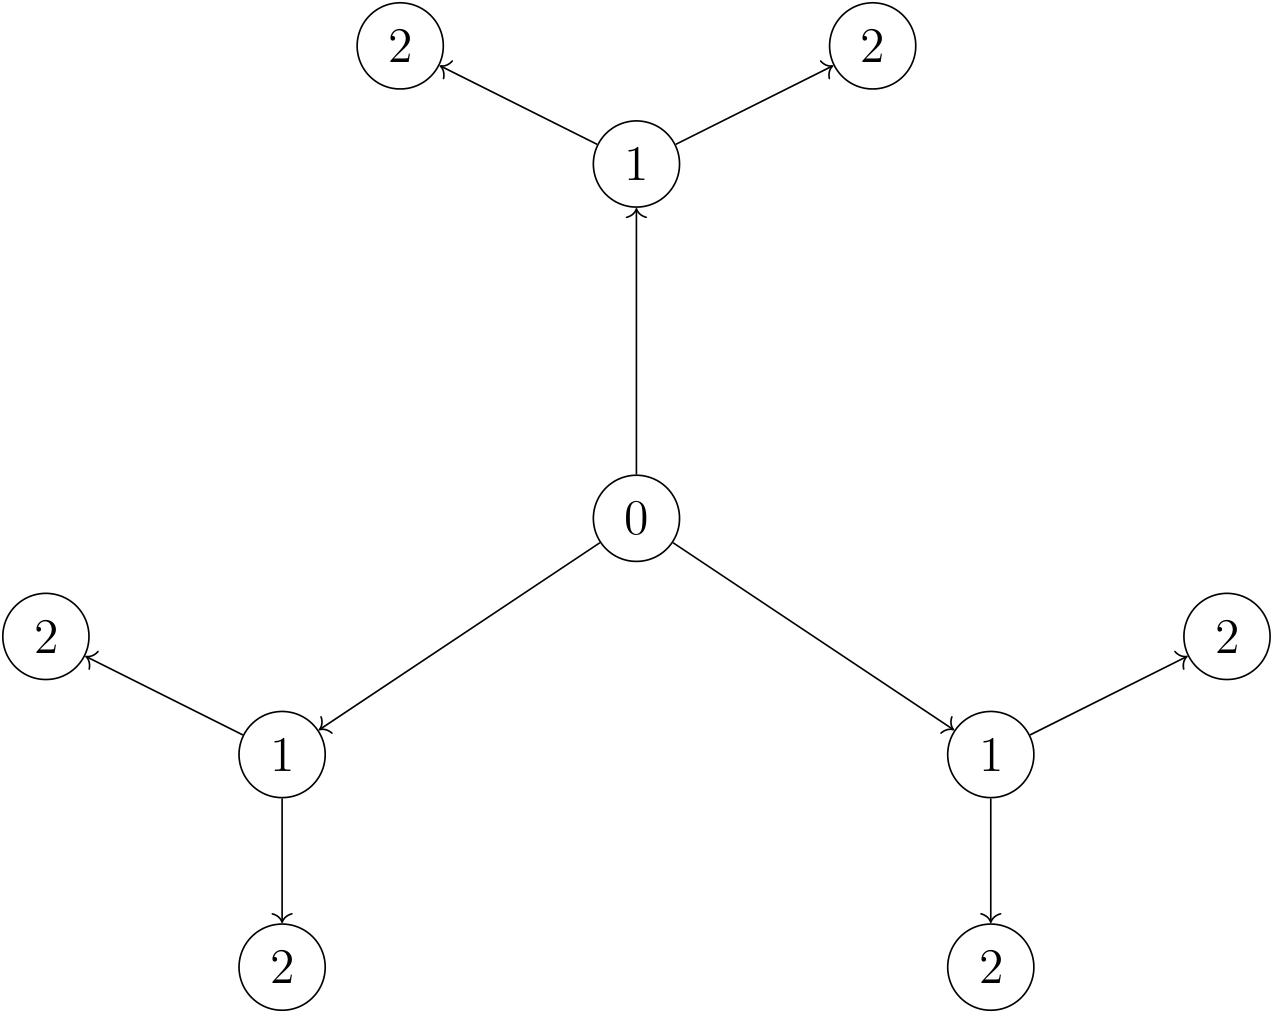
\includegraphics[width=0.36\textwidth]{figures/f61-tree.png}
\end{center}
Hecke 代数 $H(\mathrm{PGL}_2)$ 从右侧作用在它上面，Hecke 算子 $T$ 以下式作用在函数 $f$ 上：
\[
  Tf(x)=\sum_{y\sim x}f(y),
\]
其中 $x$ 是树的一个顶点，$y\sim x$ 表示与它相邻的顶点 $y$。于是对 $\mathrm{PGL}_2(O)\backslash\mathrm{PGL}_2(F)/\mathrm{PGL}_2(O)$ 有同构
\[
  X(F)/G(O)=\mathrm{PGL}_2(O)\backslash\mathrm{PGL}_2(F)/\mathrm{PGL}_2(O)\simeq\mathbb Z_{\ge0}.
\]
因此 $X(F)/G(O)$ 上的函数就是树上的径向函数。已知 $T_l=T_r$，记作 $T$。$T$ 的作用可以这样图示：固定中心顶点，让其余顶点绕中心旋转。$T$ 对函数 $f$ 的作用由下式给出
\[
  Tf(0)=(q+1)f(1),\qquad Tf(1)=f(0)+qf(2),\qquad Tf(n)=f(n-1)+qf(n+1).
\]
我们有如下对应：
\[
  C_c(X(F))^{G(O)}\longrightarrow\mathbb C[\mathrm{Sl}_2/\mathrm{conj}].
\]
左端是 A 侧，右端是 B 侧。由于 $T_l=T_r=T$（两个 Hecke 算子重合），B 侧的 $\mathrm{Sl}_2/\mathrm{conj}$ 落在 $\mathrm{Sl}_2\times\mathrm{SL}_2/\mathrm{conj}$ 的对角线上。

可以验证：A 侧的 $1$ 被送到 B 侧的 $1$；A 侧的 Hecke 算子被送到 B 侧的乘法；并且
\[
  \langle f,f\rangle=\int_{SU_2/\mathrm{conj}}f\cdot(\mathrm{SL}_2\ \text{的}\ q\text{-特征标})\cdot\text{Haar 测度},
\]
其中 $SU_2$ 是 $\mathrm{SL}_2$ 的极大紧子群。

\section{第二日第四讲}

我们主要研究 $\mathbb F_q$ 上的曲线 $\Sigma$，从我们的观点看它是 2 维算术对象。对 $\mathbb F_q$ 上的曲线 $\Xi$（3 维算术对象），用 $\Sigma\times S^1$ 可得类似的陈述。

在第二日第一讲里，我们描述了如何把 $A_G(\Sigma)$ 变成 $A_G(S^2)$-模（或者按某些人的偏好，变成一个 actegory，即作用范畴）。让我们回顾这个构造。取一点 $x\in\Sigma$，从 $\Sigma\times[0,1]$ 中挖去中心在 $(x,\frac12)$ 的小球。现在可以把它看作从 $\Sigma\sqcup S^2$ 到 $\Sigma$ 的配边。

现在对之作 $A_G$，得到函子 $A_G(S^2)\otimes A_G(\Sigma)\to A_G(\Sigma)$。由于 $A_G(S^2)$ 带有幺半结构（第一日第一讲引入），映射 $A_G(S^2)\otimes A_G(\Sigma)\to A_G(\Sigma)$ 使 $A_G(\Sigma)$ 具有 $A_G(S^2)$-模结构。

当 $\mathcal F_G(\Sigma)=\Bun_G(\Sigma)$ 时有个问题：$\Bun_G$ 是代数几何对象，而 $\Sigma\times[0,1]$ 是拓扑空间，没有代数簇结构。为修补这一点，我们把图中的区间进一步收缩，只在 $\Sigma$ 内留下一个小「泡」（对应此前挖掉的开球）。

\begin{center}
  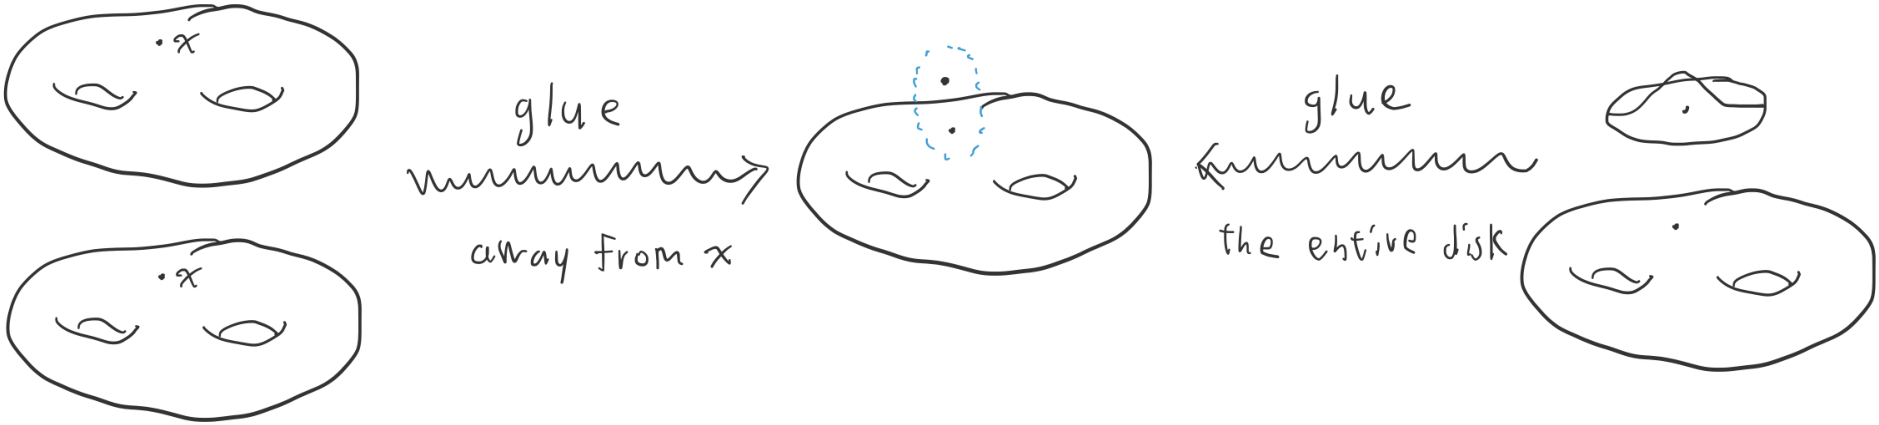
\includegraphics[width=0.92\textwidth]{figures/f71-collapse.png}
\end{center}

更形式地说，这是非分离代数簇「$\Sigma$ 带一个双点」。它可以用下面任一种方式等价描述：
\[
  \Sigma\sqcup_{\Sigma\setminus x}\Sigma=\Sigma\sqcup_D(D\sqcup_{D^\times}D).
\]
这里 $D=\Spec\mathbb F_q[[t]]$ 是形式圆盘，$D^\times=\Spec\mathbb F_q((t))$ 是去心形式圆盘，都以 $x$ 为中心。我们把 $D\sqcup_{D^\times}D$ 称作一个 \textbf{raviolo}，为简单起见记作 $R$。

注意描述 $\Sigma\sqcup_D(D\sqcup_{D^\times}D)$ 现在在代数几何中说得通。我们得到 Hecke 对应
\[
  \begin{array}{ccc}
    & \Bun_G(\Sigma\sqcup_{\Sigma\setminus x}\Sigma=\Sigma\sqcup_D R) & \\[2pt]
    \swarrow & & \searrow \\[2pt]
    \Bun_G(\Sigma)\times\Bun_G(R) & & \Bun_G(\Sigma)
  \end{array}
\]
它由把 $G$-丛限制到簇的相应部分给出。（顶点 $\Bun_G(\Sigma\sqcup_D R)$ 也叫 Hecke 栈。）这是意料之中的：$\Sigma_1$ 与 $\Sigma_2$ 之间的配边应当给出 $\mathcal F_G(\Sigma_1)$ 与 $\mathcal F_G(\Sigma_2)$ 之间的对应。把该对应线性化，得到映射
\[
  A_G(R)\otimes A_G(\Sigma)\to A_G(\Sigma),
\]
也就是说，在 2 维情形这是一个函子；若取 3 维的 $\Xi$ 代替 $\Sigma$，它就是代数同态。回忆 $A_G(\Sigma)=\Shv(\Bun_G(\Sigma))$，其中 $\Shv$ 是某种可构造层范畴：de Rham、Betti 或 étale。

要理解 Langlands，我们首先得理解 $A_G(R)$，它常被称为 Hecke 算子范畴（简称 Hecke 范畴）。为此我们需要几何 Satake 等价。

\begin{rem}
在第一日第一讲中，$A_G(S^2)$ 上有一个幺半结构，它把 $A_G(\Sigma)$ 变成 $A_G(S^2)$-模。用 raviolo 可以同样地操作。现在考虑中心有三个叠置点的 raviolo
\[
  X=D_1\sqcup_{D^\times}D_2\sqcup_{D^\times}D_3.
\]
这是一个（非分离）簇，带有三个自然映射 $p_{12},p_{13},p_{23}$ 到 raviolo $R$（把三个叠置点中任意两个相撞）。定义 $m:A_G(R)\otimes A_G(R)\to A_G(R)$ 为
\[
  m=p_{13,*}(p_{12}^*\otimes p_{23}^*)
\]
（照例，这里的某个 $*$ 可能是 $!$）。当然，我们在此省略了一些细节，因为最后的推前严格说来并不成立（它的定义域是 $A_G(X)$ 而不是 $A_G(X)\otimes A_G(X)$）。

与真正的 $S^2$ 的情形类似，可以证明 $A_G(R)$ 是一个 $E_3$-范畴（这里有一些代数几何的技术细节）。特别地，$A_G(R)$ 是对称幺半范畴。

也可以给图景加上分歧。作用是一样的：在中间切一个球。无分歧点处的代数/范畴也一样。然而在分歧点 $x_0\in\Sigma$ 处，球无法离开区间 $x_0\times[0,1]$，于是我们没有 $E_3$-结构。
\end{rem}

我们再引入一些记号：记 $F=\mathbb F_q((t))$，$O=\mathbb F_q[[t]]$ 为 $F$ 的整数环。

我们用双陪集来描述 $A_G(R)=\Shv(\Bun_G(R))$。回忆 $R=D_1\sqcup_{D^\times}D_2$。$R$ 上一个 $G$-丛（同构意义下）由以下数据给出：每个 $D_i$ 上的一个 $G$-丛，加上一个粘接函数 $g:D^\times=D_1\cap D_2\to G$。$D_i$ 上的丛总是平凡的，而粘接函数按定义就是 $G(F)$ 中的元素。此外，两个粘接函数 $g,g'$ 定义同构的 $G$-丛，当且仅当 $g'=h_1gh_2^{-1}$ 对某个 $h_1,h_2\in G(O)$ 成立。因此我们刚刚证明了

\begin{lem}
  $\Bun_G(R)=G(O)\backslash G(F)/G(O)$。
\end{lem}

\begin{rem}
设 $G$ 半单。利用一个（更难的）事实：射影的 $\Sigma$ 上任何主 $G$-丛都在某点之外平凡化（这归功于 Harder），可以把论证搬到一般的 $\Bun_G(\Sigma)$ 上。这与本讲无关。
\end{rem}

注意 $G(F)/G(O)=LG/L^+G=\Gr$ 按定义就是 $G$ 的仿射 Grassmann 流形。于是 $\Bun_G(R)=G(O)\backslash\Gr=\Gr$ 是 $G$ 的「$G(O)$-等变仿射 Grassmann 流形」。因此 Hecke 范畴 $A_G(R)$ 是
\[
  H=\Shv(\Gr)=\Shv_{G(O)}(\Gr),
\]
即仿射 Grassmann 流形上 $G(O)$-等变可构造层的（导出）范畴。在 3 维情形，我们将得到 Hecke 代数 $H=\Fun(\Gr(\mathbb F_q))$。

在第二日第二讲里我们讨论了经典 Satake 同构：
\[
  \Fun(\Gr/\mathbb F_q)\cong K_0(\Rep\check G)\cong O(\check G/\check G)=O(\Maps(S^1,*/\check G)).
\]
现在我们把该同构范畴化，先得到几何 Satake 等价，再得到导出几何 Satake 等价。

考虑仿射 Grassmann 流形上 $G(O)$-等变反常层（perverse sheaves）的 Abel 范畴，记作 $\Shv(\Gr)^\heartsuit$。同样地，可以用任何层论：étale、Betti 或 de Rham。文献中也用记号 $\mathrm{Perv}(\Gr)$。（事实上按定义，$\mathrm{Perv}(\Gr)$ 就是 $G(O)$-等变可构造层导出范畴 $\Shv(\Gr)$ 上 $t$-结构的核心。）

\begin{thm}[几何 Satake 等价]
存在对称幺半范畴的等价
\[
  \Shv(\Gr)^\heartsuit\cong\Rep(\check G),
\]
其中 $\Shv(\Gr)^\heartsuit$（相应地 $\Rep(\check G)$）上的幺半结构是反常层的卷积（相应地表示的张量积）。
\end{thm}

\begin{rem}
  \begin{enumerate}[label=(\arabic*),leftmargin=1.8em,itemsep=0.2em]
    \item 注意两个范畴都带有到向量空间的自然函子：遗忘函子
    \[
      \Rep(\check G)\to\Vect,
    \]
    与上同调函子
    \[
      H^*_{G(O)}(\Gr,-):\ \Shv(\Gr)^\heartsuit\to\Vect
    \]
    （用 $t$-结构定义）。它们称为纤维函子，而几何 Satake 等价与这两个函子相容。但若用 $\mathrm{GrVect}$（分次向量空间）代替 $\Vect$，则需要 Koszul 符号法则。
    \item 把该等价取到 Grothendieck 环 $K_0$ 的层面（或取恒等函子的迹），就恢复出经典 Satake 同构。
    \item 作为对称幺半范畴的等价，它特别地意味着 $\Shv(\Gr)^\heartsuit$ 上的幺半结构是交换的。下面是直接的说明。我们已看到 $\Shv(\Gr)^\heartsuit$ 是 $E_3$-范畴。范畴上的 $E_n$-结构由以 $\mathbb R^n$ 中点的构型空间为标号的一族乘法组成。随着 $n$ 增大，这些乘法变得越来越交换。$n=1$ 时得到幺半范畴；$n=2$ 时得到辫幺半范畴（即 $a\otimes b$ 同构于 $b\otimes a$，但这些同构不必是对合的）；最后当 $n=3$ 时，第一个乘法必然变成交换的，于是得到对称幺半范畴。
  \end{enumerate}
\end{rem}

由几何 Satake 等价，对任意点 $x\in\Sigma$，我们有 $\Shv(\Gr)^\heartsuit\cong\Rep\check G$ 在 $A_G(\Sigma)=\Shv(\Bun_G(\Sigma))$ 上的（受限）Hecke 作用。由于 $x\in\Sigma$ 的选取是任意的，为更典范起见，我们得把所有点都算进去。为此可以引入 $\Rep(\check G)$ 的阿代尔版本：受限张量积
\[
  \bigotimes_{x\in\Sigma}{}^{\mathrm{restr}}\,\Rep\check G.
\]
上述作用一般而言是神秘的，人们希望把它「对角化」。为此我们求助于
\[
  \bigotimes_{x\in\Sigma}{}^{\mathrm{restr}}\,\Rep\check G\ \ \text{在}\ \ \QCoh(\Loc_{\check G}\Sigma)\ \ \text{上的作用}.
\]
再说一次，任何版本的局部系（de Rham、Betti、étale）都完全适用。

\textbf{约定}：至少在本讲中，我们把谱理论（即下文所说的朴素 B-理论）的系数域取为 $\mathbb C$。

为更精确地描述该作用，先固定某个 $x\in\Sigma$。有等同
\[
  \Loc_{\check G}\Sigma=\Maps(\Sigma,*/\check G)
\]
（局部常值映射）。然后定义 $\mathrm{ev}_x:\Loc_{\check G}\Sigma\to*/\check G$ 为在 $x$ 处取值。（等价地，可以把任意 $\check G$-局部系限制到点 $x\in\Sigma$，这给出映射 $\Loc_{\check G}\Sigma\to*/\check G$。）另一方面，每个表示都定义了点上（更精确地说，$*/\check G$ 上）的一个向量丛，于是有等同
\[
  \QCoh(*/\check G)=\Vect(*/\check G)=\Rep\check G.
\]
因此给定任意表示 $V\in\Rep(\check G)$，可沿 $\mathrm{ev}_x$ 拉回，得到 $\Loc_{\check G}\Sigma$ 上的拟凝聚层 $\mathrm{ev}_x^*V$；而 $V$ 在 $\QCoh(\Loc_{\check G}\Sigma)$ 上的作用就是与 $\mathrm{ev}_x^*V$ 作张量积。这延拓为 $\bigotimes\nolimits_{x\in\Sigma}^{\mathrm{restr}}\Rep\check G$ 的真正作用。

\begin{rem}
若 $\Sigma$ 定义在 $\mathbb F_q$ 上，则对任意 $x\in\Sigma(\mathbb F_q)$ 还可以联系一个映射 $\Loc_{\check G}\Sigma\to\check G/\check G$。这是因为 Frobenius 态射扮演了 $S^1$ 的角色。
\end{rem}

天真地，人们可以把几何 Langlands 对应表述为：作为 $\bigotimes\nolimits_{x\in\Sigma}^{\mathrm{restr}}\Rep\check G$-模，$\Shv(\Bun_G(\Sigma))$ 与 $\QCoh(\Loc_{\check G}\Sigma)$ 是否等价？
答案是否定的。关键原因是：$\bigotimes\nolimits_{x\in\Sigma}^{\mathrm{restr}}\Rep\check G$ 在 $\QCoh(\Loc_{\check G}\Sigma)$ 上的作用是局部常值的，而在 $\Shv(\Bun_G(\Sigma))$ 上的作用完全不是局部常值的。

为了有等价，我们要么把右端换成 $\IndCoh(\Loc_{\check G}\Sigma)$（ind-凝聚层），要么把左端换成 tempered 层。

\begin{rem}
对每种层论（de Rham、Betti 与 étale），都有一个谱作用定理，它们大致都可以概括为下面这条。
\end{rem}

\begin{thm}[谱作用]
$\bigotimes\nolimits_{x\in\Sigma}^{\mathrm{restr}}\Rep\check G$ 在 $A_G(\Sigma)=\Shv(\Bun_G(\Sigma))$ 上的作用经过 $\QCoh(\Loc_{\check G}\Sigma)$-作用分解。
\end{thm}

尽管如此，让我们（暂时）朴素地研究 $\QCoh(\Loc_{\check G}\Sigma)$。于是我们考虑 B-理论：它给 2 维流形 $\Sigma$ 配 $B_{\check G}(\Sigma)=\QCoh(\Loc_{\check G}\Sigma)$，给 3 维流形 $\Xi$ 配向量空间 $B_{\check G}(\Xi)=O(\Loc_{\check G}\Xi)$。与 A-理论不同，这定义了真正的 TQFT：输出只依赖 $\Sigma$ 或 $\Xi$ 的拓扑。

与 A-理论一样，我们得先花点时间看 $B_{\check G}(R)$。由于 raviolo 不过是一个带双点的圆盘，可以把 $R$ 上的局部系等同于圆盘 $D^2$ 上的一对局部系，连同它们在 $S^1=\partial D^2$ 上的一个等同。于是可以算出
\[
  \Loc_{\check G}(R)=\Loc_{\check G}(D^2)\times_{\Loc_{\check G}(S^1)}\Loc_{\check G}(D^2).
\]
若暂时取 Betti 作为层论，则得到（栈的）等同
\[
  \Loc_{\check G}(D^2)=\{\pi_1(D^2)\to\check G\}/\check G=*/\check G,\qquad
  \Loc_{\check G}(S^1)=\{\pi_1(S^1)\to\check G\}/\check G=\check G/\check G
\]
（两处 $\check G$ 都按共轭作用）。它们给出等同
\[
  \Loc_{\check G}(R)=*/\check G\times_{\check G/\check G}*/\check G=(*\times_{\check G}*)/\check G.
\]
这里点 $*$ 作为单位元映入 $\check G$。因此取纤维积 $*\times_{\check G}*$ 时只用到单位元的邻域。由此可见可以把 $\check G$ 换成它的 Lie 代数 $\check{\mathfrak g}$，得到等同
\[
  *\times_{\check G}*=*\times_{\check{\mathfrak g}}*=\Omega\check{\mathfrak g},
\]
其中 $\Omega\check{\mathfrak g}$ 是 $\check{\mathfrak g}$ 的环路空间。

对一般的向量空间 $V$，$*\times_V*$ 是点 $*$ 的自交。对通常的代数簇，我们会算
\[
  *\times_V*=\Spec\mathbb C\times_{\Spec\Sym V^*}\Spec\mathbb C=\Spec(\mathbb C\otimes_{\Sym V^*}\mathbb C).
\]
但我们工作在导出情形，这意味着最后一步应取导出张量积。写出 Koszul 复形即可看出，$\mathbb C\otimes^L_{\Sym V^*}\mathbb C$ 是 $\dim V$ 个次数为 $1$ 的变量的外代数。可以验证两侧的乘法相同，且有自然同构
\[
  \mathbb C\otimes^L_{\Sym V^*}\mathbb C=\Sym V^*[1].
\]
这里 $1$ 是上同调移位，特别地 $\Sym V^*[1]$ 是外代数。

于是近似地，$B_{\check G}(R)$ 就是 $\QCoh(\Loc_{\check G}(R))=\Sym\check{\mathfrak g}^*[1]\text{-}\mathrm{Mod}_{\check G}$。注意幺半结构不是模的张量积，而是由
\[
  \Loc_{\check G}(R)=*/\check G\times_{\check G/\check G}*/\check G
\]
是同一栈的两份拷贝的纤维积这一事实而来的卷积。这一点可以用幺半结构的「裤子」（pair of pants）定义验证。

\begin{rem}[Koszul 对偶]
给定带增广 $\epsilon:\Lambda\to k$ 的外 $k$-代数 $\Lambda$，考虑函子 $\Hom_\Lambda(k,-):\Lambda\text{-}\mathrm{Mod}\to\End_\Lambda(k)\text{-}\mathrm{Mod}$。其中
\begin{enumerate}[label=(\arabic*),leftmargin=1.8em,itemsep=0.2em]
  \item $\Lambda\text{-}\mathrm{Mod}$ 上的幺半结构由卷积给出：给定两个 $\Lambda$-模，沿 $\epsilon$ 把它们推到 $k$-模，取张量积，再沿 $\epsilon$ 拉回；
  \item $\End_\Lambda(k)$ 对 $\Hom_\Lambda(k,M)$ 的作用由与自同态作前复合给出。
\end{enumerate}
除非仔细规定所考虑的模的类别，这个函子并不是模的导出范畴的等价。事实上，它限制为凝聚 $\Lambda$-模与完美 $\End_\Lambda(k)$-模之间的等价。

上面的 Koszul 对偶可以提升到局部算子范畴，建立等价
\[
  \Coh(\Loc_{\check G}(R))\cong\Perf(\check{\mathfrak g}^*[2]/\check G).
\]
把这两个范畴作 ind-完备化，又得到
\[
  \IndCoh(\Loc_{\check G}(R))\cong\QCoh(\check{\mathfrak g}^*[2]/\check G)
\]
之间的等价。这是幺半范畴的等价：右端带有通常的幺半结构，而左端相应的幺半结构是从 $\Omega\check{\mathfrak g}$ 的群胚结构而来的卷积。
\end{rem}

回到 A-与 B-理论，我们准备陈述几何 Satake 等价的导出版本（不带核心的那一个）。我们天真地要求 $A_G(R)=\Shv(\Gr)$ 与 $B_{\check G}(R)=\QCoh(\Loc_{\check G}R)$ 之间的等价。正如已经说过的，这并不正确，正确版本如下。

\begin{thm}[导出几何 Satake 等价]
存在对称幺半范畴的等价
\[
  \Shv(\Gr)\cong\IndCoh(\Omega\check{\mathfrak g}/\check G)=\QCoh(\check{\mathfrak g}^*[2]/\check G).
\]
\end{thm}

\begin{rem}
\begin{enumerate}[label=(\arabic*),leftmargin=1.8em,itemsep=0.2em]
  \item 提请注意：导出几何 Satake 等价的右端出现了余伴随表示，这是诸多迹象之一，说明矩映射（进而 Hamilton 作用）将在我们的故事中起作用。这将在此后各讲中成为一个大主题。
  \item 与几何 Satake 等价的情形类似，导出几何 Satake 等价中的范畴也带有纤维函子。在仿射 Grassmann 流形一侧，可以取等变上同调
  \[
    H^*_{G(O)}(\Gr,-):\ \Shv(\Gr)\to H^*_{G(O)}(\mathrm{pt})\text{-}\mathrm{Mod}.
  \]
  另一侧有函子
  \[
    \QCoh(\check{\mathfrak g}^*[2]/\check G)\to O(\check{\mathfrak g}^*[2]/\check G)\text{-}\mathrm{Mod},
  \]
  由限制到 Kostant 切片给出（这里不作解释）。由若干计算可知
  \[
    \begin{aligned}
      O(\check{\mathfrak g}^*[2]/\check G)&=O(\check{\mathfrak g}^*[2])^{\check G}=\Sym\check{\mathfrak t}[2]^W=\Sym\mathfrak t^*[2]^W\\
      &=\Sym\mathfrak t[-2]^W=\Sym\mathfrak g[-2]^G=H^*_{G(O)}(\mathrm{pt}).
    \end{aligned}
  \]
  同样地，该等价与这两个纤维函子相容。
\end{enumerate}
\end{rem}

\section{第三日第一讲}

我们还没有谈过球簇，它在 BZSV 的故事里有重要地位。这里我们不打算一上来就给出定义，而是通过考察「什么样的簇让我们能够推广此前见到的调和分析」来引出它。

设 $G$ 是非 archimedean 域 $F$ 上的分裂约化群，$O$ 是赋值环，剩余域为 $\mathbb F_q$。记
\[
  H_G:=H(G(F),G(O))
\]
为 Hecke 代数，把它看作 $G(F)$ 上紧支集 $G(O)$-双不变函数的空间，乘法由 $G$ 上 Haar 测度的卷积给出。由 Satake 同构，有同构
\[
  H_G\xrightarrow{\ \sim\ }\mathbb C[\Rep\check G],\qquad f\mapsto\hat f,
\]
其中右端指张量范畴 $\Rep_{\mathbb C}\check G$ 的 Grothendieck 环 $K_0$ 上的群代数。

现在作升级。设 $X$ 是带 $G$ 作用的光滑仿射空间。可以考虑紧支集局部常值函数空间 $C_c^\infty(X(F))$，我们称之为 $X$ 的「Schwartz 空间」，记作 $\mathcal S(X(F))$。它自然是 $G(F)$-表示。再考虑右 $G(O)$-不变子空间
\[
  \mathcal S(X(F))^{G(O)}:=C_c^\infty(X(F))^{G(O)},
\]
它是 Hecke 代数 $H_G$ 右作用的模。（这叫 $X(F)$ 的「球」Schwartz 空间。）但我们此前也看到，其实应当把这个向量空间看作内积空间：
\[
  \mathcal S(X(F))^{G(O)}\subset\big(L^2(X(F)),\langle\ ,\ \rangle\big),
\]
其中乘积按 $X(F)$ 上的不变测度积分。（另一种做法是把 $L^2$ 空间取成 $X(F)$ 上的半密度，此时球 Hecke 代数中的函数 $f$ 要写成 $f|dx|^{1/2}$。）记
\[
  \mathbf 1_X:=\mathbf 1_{X(O)}
\]
为 $X(O)$ 的示性函数。这是 Schwartz 空间中的「基本向量」。（一般地，这个基本函数的公式在 $X$ 光滑时是好的。对于非光滑簇（不在本文范围内），基本向量应当与 $X$ 的环路空间的 IC 层相关联。）

在此前的讲座与练习中，我们已经遇到过球 Schwartz 空间中内积的两个例子：

\begin{exmp}
  设 $X=\mathbb A^1$，$G=\mathbb G_m$ 按伸缩作用。$\mathbb A^1$ 中的 $G(O)$-轨道恰是环带 $\{x\in\mathbb A^1(F):|x|=q^{-n}\}_{n\in\mathbb Z}$，而球 Schwartz 空间由这些环带的示性函数的有限组合构成。Hecke 代数是 $H_G\simeq\mathbb C[\mathbb Z]\xrightarrow{\sim}\mathbb C[\mathbb C^\times]$。（这里不可避免地有个记号冲突：$\mathbb C[\mathbb Z]$ 指 $\mathbb Z$ 的群代数，而 $\mathbb C[\mathbb C^\times]$ 指 $\mathbb C$ 上 $\mathbb C^\times=\mathbb G_m$ 的代数函数。）由此可见 Satake 变换是一种 Fourier 变换，我们把它记作 $h\in H_G\mapsto\hat h\in\mathbb C[\mathbb C^\times]$。于是 $\mathcal S(X(F))$ 中的内积用 Satake 变换写出来如下：
  \begin{equation}
    \langle h\star\mathbf 1_X,\mathbf 1_X\rangle
    =\int_{S^1\subset\mathbb C^\times}\frac{\hat h(z)}{(1-q^{-1/2}z)(1-q^{-1/2}z^{-1})}\,d^\times z
    \label{eq:8-2}
  \end{equation}
  其中 $d^\times z=\frac{dz}{z}$ 是乘法 Haar 测度。注意我们做作业时已经见过这个 q-特征标。
\end{exmp}

\begin{defn}
  量 $\dfrac{d^\times z}{(1-q^{-1/2}z)(1-q^{-1/2}z^{-1})}$ 称为 $\mathbf 1_{\mathbb A^1}$ 的 \textbf{Plancherel 密度}。
\end{defn}

让我们回顾这个 q-特征标在「对偶」（即 $B$）侧是如何出现的。一般地 $M=T^*X$，所以这里 $M=T^*\mathbb A^1$。对偶地，我们得到 $\check G=\mathbb G_m$，它作用在 $\check M$ 上，而 $\check M$ 恰好也等于 $T^*\mathbb A^1$。作用按权 $(1,-1)$ 进行，即
\[
  \lambda.(x,y)\mapsto(\lambda x,\lambda^{-1}y)\in T^*\mathbb A^1=\mathbb A^1\times(\mathbb A^1)^*.
\]
（这里 $\mathbb G_m$ 与 $T^*\mathbb A^1$ 各自带有一个例外的自对偶；一般地，$\check G$ 与 $\check M$ 会和 $G$ 与 $M$ 很不一样。）

回顾 q-特征标的定义：
\begin{equation}
  \mathrm{q\text{-}tr}(z)=\sum_{i\ge0}q^{-i/2}\operatorname{tr}\big(z\,|\,\mathbb C[\check M]_i\big)
  =\frac{1}{\det(I-q^{-1/2}z\,|\,\check M)},
  \label{eq:8-4}
\end{equation}
其中 $\mathbb C[\check M]_i=\Sym^i(\check M^\vee)=\Sym^i(\check M)$（用到 $\check M=\mathbb A^1\times(\mathbb A^1)^*$ 作为向量空间的线性自对偶）。这里的分次来自我们即将称之为 $G_{\mathrm{gr}}$ 的作用，它把 $\check M$ 的两个 $\mathbb A^1$ 因子按同一比例伸缩（即 $G_{\mathrm{gr}}$ 按权 $(1,1)$ 作用）。由于 $G_{\mathrm{gr}}$ 同构于 $\mathbb G_m$，这可能引起混淆；所以我们在此强调：$\check M$ 上有\textbf{两个不同}的 $\mathbb G_m$ 作用，即 $\check G=\mathbb G_m$ 的作用与 $G_{\mathrm{gr}}=\mathbb G_m$ 的作用。

总结一下：表达式 $\dfrac{1}{(1-q^{-1/2}z)(1-q^{-1/2}z^{-1})}$ 是 $\check M=T^*\mathbb A^1$ 在 $G_{\mathrm{gr}}$-分次下的 q-特征标。我们把它记作 $L(z,\check M)$。一般地，Plancherel 密度形如
\[
  \text{Plancherel 密度}=(\text{辛簇}\ \check M\ \text{的 q-特征标})\,d^\times z=L(z,\check M)\,d^\times z,
\]
于是 (8.2) 可以重写为
\begin{equation}
  \langle h\star\mathbf 1_X,\mathbf 1_X\rangle=\int_{S^1\subset\mathbb C^\times}\hat h(z)\,L(z,\check M)\,d^\times z.
  \label{eq:8-5}
\end{equation}
我们希望这条公式对更一般的一类 $G$-簇 $X$ 也成立，其中 $M=T^*X$，对偶为 $\check G_X,\check M$。（注意 Plancherel 密度的公式里只出现 $\check M$——特别地，若多个 $G$-簇 $X$ 给出同一个 $\check G_X$ 与 $\check M$，则它们基本向量的 Plancherel 密度应当相同。）

\textbf{注}（给算术背景的读者）。我们的公式里有很多 $q^{1/2}$；这提示在 $\mathbb C$ 以外的域上工作时，必须选定一个 $q$ 的平方根。算术设定中的这种歧义由所谓的 $C$-群（而不是 $L$-群）来消解。当然在 $\mathbb C$ 上，可以取正的 $q^{1/2}$。

\begin{exmp}
  设 $X=H$，$G=H\times H$，其中 $H$ 是分裂约化群。双模结构为 $(h_1,h_2)\in G:x\in X\mapsto h_1^{-1}xh_2$。Schwartz 空间恰好就是 $H$ 的 Hecke 代数：
  \[
    \mathcal S(X)^{G(O)}\cong H_H.
  \]
  在对偶侧，我们得到 $\check G=\check H\times\check H$ 与 $\check G_X=\check H$。于是有反对角嵌入
  \[
    \check G_X=\check H\xrightarrow{(C,\mathrm{Id})}\check H\times\check H=\check G,\qquad a\mapsto(a^{-1},a),
  \]
  其中 $C$ 表示 Cartan 对合。于是在经典 Satake 变换下，Hecke 代数的等同变为
  \[
    H_G=H_H\otimes H_H\cong\mathbb C[\check H]^{\check H},\qquad h_1\otimes h_2\mapsto\hat h_1(z^{-1})\cdot\hat h_2(z).
  \]
  于是此情形下的内积读作
  \begin{equation}
    \langle(h_1\otimes h_2)\star\mathbf 1_H,\mathbf 1_H\rangle
    =\int_{\check H_c}\frac{\hat h_1(z^{-1})\hat h_2(z)}{\det(I-q^{-1}z\,|\,\check{\mathfrak h})}\,d_{Haar}(z)
    \label{eq:8-7}
  \end{equation}
  \begin{equation}
    \phantom{\langle(h_1\otimes h_2)\star\mathbf 1_H,\mathbf 1_H\rangle}
    =\int_{\check H_c}\hat h_1(z^{-1})\hat h(z)\,L(z,\check{\mathfrak h})\,d_{Haar}(z).
    \label{eq:8-8}
  \end{equation}
  下面澄清积分中出现的各项。我们在对偶群 $\check H$ 的紧形式 $\check H_c$ 上积分，$d_{Haar}(z)$ 表示 Haar 测度。记 $\check{\mathfrak h}=\mathrm{Lie}(\check H)$，$L(z,\check{\mathfrak h}):=\dfrac{1}{\det(\mathrm{Id}-q^{-1}z)}$，它表示 $\check H$ 在 $\check{\mathfrak h}$ 上伴随作用的 q-特征标。最后，$\check{\mathfrak h}$ 上的分次 $G_{\mathrm{gr}}$-作用为 $\lambda.z\mapsto\lambda^2z$，即通常伸缩作用的平方（这就是分母中出现 $q^{-1}$ 而不是 $q^{-1/2}$ 的原因）。注意积分所在的群不是 $\check G_c$ 而是 $\check H_c$，这反映了此例中 $\check G_X=\check H$ 而非 $\check G$。
\end{exmp}

如我们已提到的，有一个一般的预期：对足够好的一类 $(G,X)$（$G\circlearrowleft X$），类似的故事成立。给定 $X$，我们预期存在对偶群 $\check G_X\subset\check G$，具有如下性质。我们有作用 $\mathcal S(X(F))^{G(O)}\circlearrowleft H_G$，它给出映射
\begin{equation}
  H_G\to\End\Big(\mathcal S(X(F))^{G(O)}\Big).
  \label{eq:8-9}
\end{equation}
而在 Satake 同构 $H_G\simeq\mathbb C[\Rep\check G]$ 下，其中 $\mathbb C[\Rep\check G_X]$ 表示 Grothendieck 环 $K_0(\Rep\check G_X)$ 的群代数。$\check G$ 的表示自然限制为任意子群 $\check G'\subset\check G$ 的表示；特别地，这给出自然的环同态 $\mathbb C[\Rep\check G]\xrightarrow{\text{限制}}\mathbb C[\Rep\check G']$。我们预期 $\check G_X$ 是 $\check G$ 的约化子群，使得 $H_G$ 的作用分解为：
\begin{equation}
  \begin{array}{ccc}
    H_G & \longrightarrow & \End_{\mathbb C}\big(\mathcal S(X(F))^{G(O)}\big)\\[3pt]
    \overset{\text{Satake}}{\simeq}\Big\downarrow & & \Big\uparrow\\[3pt]
    \mathbb C[\Rep\check G] & \xrightarrow{\ \text{限制}\ } & \mathbb C[\Rep\check G_X].
  \end{array}
  \label{eq:8-10}
\end{equation}
换句话说，我们预期 Hecke 代数 $H_G\simeq\mathbb C[\Rep\check G]$ 在球 Schwartz 空间上的作用「经过」它在 $\mathbb C[\Rep\check G_X]$ 上的限制分解。（注意这个限制映射未必满射。）

我们还预期「基本向量」$\mathbf 1_{X(O)}$ 作为 $H_G$-模生成整个球 Schwartz 空间 $\mathcal S(X(F))^{G(O)}$。事实上我们预期得更多。记 $\mathbb C[\Rep\check G_X]:=H_G^X$。我们预期模 $\mathcal S(X(F))^{G(O)}$ 在 $H_G^X$ 上秩 $1$ 自由，且有指定的生成元 $\mathbf 1_{X(O)}$。换句话说，可以把 (8.10) 的右侧竖直映射看作给出典范同构
\begin{equation}
  H_G^X\xrightarrow{\ \sim\ }\End_{H_G}\Big(\mathcal S(X(F))^{G(O)}\Big),
  \label{eq:8-11}
\end{equation}
或者，由于 $\mathcal S(X(F))^{G(O)}$ 中有指定的向量，我们得到向量空间的自然同构
\begin{equation}
  H_G^X\xrightarrow{\ \sim\ }\mathcal S(X(F))^{G(O)},
  \label{eq:8-12}
\end{equation}
它把
\begin{equation}
  \mathbb C[\Rep\check G_X]\ni\mathrm{Triv}\mapsto\mathbf 1_{X(O)}\in\mathcal S(X(F))^{G(O)}.
  \label{eq:8-13}
\end{equation}
在此等同下，$\mathcal S(X(F))^{G(O)}$ 从左端继承的乘法来自融合（fusion）。（事实上，当 $X$ 不是群时，$X$ 上的卷积根本没有意义。）

最后我们指出：为代数 $\End_{H_G}(\mathcal S(X(F))^{G(O)})$（或在上述等同下，$X(F)$ 上右 $G(O)$-等变反常层的范畴）发展 Tannakian 形式化，将把我们引向 $\check G_X$ 的 Gaitsgory--Nadler 构造。

对 $h\in H_G$，记 $\hat h$ 为其经典 Satake 变换，我们把它（通过迹）看作 $\check G$ 上的代数（类）函数。我们的预期是：
\begin{equation}
  \langle\mathbf 1_{X(O)}\star h,\mathbf 1_{X(O)}\rangle
  =\int_{\check G_{X,c}\subset\check G_X}\hat h(z)\,L(z,V_X)\,d_{Haar}z,
  \label{eq:8-14}
\end{equation}
更一般地，
\begin{equation}
  \langle\mathbf 1_{X(O)}\star h_1,\mathbf 1_{X(O)}\star h_2\rangle
  =\int_{\check G_{X,c}\subset\check G_X}\hat h_1(z)\hat h_2(z)\,L(z,V_X)\,d_{Haar}z,
  \label{eq:8-15}
\end{equation}
其中 $\check G_{X,c}$ 表示 $\check G_X\subset\check G$ 的紧形式的实点，$V_X$ 表示 $\check G_X$ 的一个 $G_{\mathrm{gr}}$-分次表示，$L(z,V_X)$ 是推广了 q-特征标的适当局部 L-因子。注意 (8.15) 的右端只看到 $\hat h$ 在 $\check G_X$ 上的限制值（事实上是在 $\check G_X$ 的紧形式上的限制值），而按定义 $\hat h$ 是 $\check G$ 上的函数。

在 Satake 变换下要保持内积，就必须纳入 L-因子（而它又依赖于 $G_{\mathrm{gr}}$-分次）；这反映了导出 Satake 等价的几何本性，将在其他讲座中讨论。关键想法是：范畴化之后，内积变成 Hom（或 Ext）群，而 $G_{\mathrm{gr}}$-分次对应于 $X(F)$ 上等变层导出范畴中的一次 \textbf{shearing}（斜框）。

但我们还是回到这个问题：哪些 $G$-簇可能满足上述种种期望？结果表明，这些期望极大地限制 $X$ 的类别。特别地，它们蕴含：对一切特征标 $\chi:H_G\to\mathbb C$（等价地，对一切 $\chi\in\check A//W_G(\mathbb C)$，其中 $\check A$ 是对偶环面），
\begin{equation}
  \dim\Hom_{H_G}\big(\Func(X(F),\mathbb C),\mathbb C_\chi\big)<\infty.
  \label{eq:8-16}
\end{equation}
例如，取 $X=G$，且只考虑 $G$ 在自身上的左作用，则由 Peter--Weyl 有
\begin{equation}
  \Fun(G(F))=\int^{\oplus}\pi\otimes e_\pi\,d\pi,
  \label{eq:8-17}
\end{equation}
它对每个特征标都不满足 (8.16)（因为对多数不可约表示 $\pi$ 有 $\dim(\pi)=\infty$）。

\textbf{断言}。设 $G$ 分裂。则有限性条件 (8.16) 成立，当且仅当 $X$ 是球簇。

这就是球簇这一类进入 BZSV 框架的缘由。

\begin{defn}
  正规不可约 $G$-簇 $X$ 称为\textbf{球簇}，若某个（等价地，任一）Borel 子群 $B\subset G$ 的作用有开稠轨道。
\end{defn}

不失一般性，此后我们假定所有球簇都是拟仿射的。这不损失一般性，因为总可以化归到这种情形——代价是引入一个交换的 $G_{\mathrm m}^N$ 作用在 $X$ 上。事实上，设给定射影嵌入 $X\to\mathbb P^N$。考虑通常的满射 $V^*:=V\setminus\{0\}\to\mathbb P^N$（$V=\mathbb A^{n+1}$），并用笛卡尔图中的 $\tilde X$ 替换 $X$：
\[
  \begin{array}{ccc}
    G\times G_{\mathrm m}^N\ \circlearrowleft & \tilde X & \longrightarrow\ V^*\\
    & \Big\downarrow & \Big\downarrow\\
    G\ \circlearrowleft & X & \longrightarrow\ \mathbb P^N.
  \end{array}
\]
例如，可以把旗簇 $G/B$（带左 $G$ 作用）换成基本的仿射空间 $G/N$，看作 $G\times A$-簇（$A$ 是极大环面）。

\begin{thm}
  $X$ 是（拟仿射）球 $G$-簇，当且仅当 $F[X]$（$X$ 的正则函数环）作为 $G$-模是重数自由的。
\end{thm}
\begin{proof}
  （$\Rightarrow$。）固定 $B\subset G$。此后我们假定 $G$ 从右作用。注意 $F[X]$ 是 $G$ 的（无限维）局部有限表示，因此分解为最高权模 $V_\chi$ 的直和，其中 $\chi$ 是 $B$ 的特征标（即 $A$ 的特征标沿自然满射 $B\twoheadrightarrow A$ 拉回）。我们要证明 $V_\chi$ 的重数为 $1$。设 $f_\chi$ 是 $V_\chi$ 中的最高权向量，看作 $X$ 上的函数。由于 $B$ 经 $\chi$ 作用在 $f_\chi$ 上，故对一切 $x\in X$、$b\in B$ 有 $f_\chi(xb)=\chi(b)f_\chi(x)$。因此 $f_\chi$ 在 $X$ 中任一 $B$-轨道上的取值由它在一点处的取值决定。而按假设 $X$ 有稠的 $B$-轨道，故 $f_\chi$ 在这个稠轨道上（从而在整个 $X$ 上）只差一个标量就被唯一确定。换言之，$F[X]$ 中任何别的 $(B,\chi)$-本征向量都只能与 $f_\chi$ 相差一个标量，这就证明了 $(B,\chi)$-本征向量在 $F[X]$ 中的重数为 $1$，从而 $V_\chi$ 在 $F[X]$ 中的重数为 $1$，如所愿。
\end{proof}

要研究球簇，我们考察两件事：(1) 稠 $B$-轨道，记作 $\mathring X$；(2) 补集 $X\setminus\mathring X$。首先，若 $x\in\mathring X$ 任意，则 $\mathring X\simeq B_x\backslash B$。注意换一个 $x\in X$ 会得到 $B$ 的共轭子群。

现在考虑 $X$ 上有理函数空间 $F(X)$。由稠密性，它与 $\mathring X$ 上的有理函数空间相同。再考虑 $F(X)$ 中 $B$-本征函数的集合，记作 $F(X)^{(B)}$。注意这些函数在 $N$ 的（右）作用下不变。我们有：
\begin{equation}
  F(X)^{(B)}\simeq F(B_x\backslash B/N)^{(A)}.
  \label{eq:8-20}
\end{equation}
由此可以定义 $A_X$，即「$X$ 的 Cartan」，它是 $A$ 在 $\mathring X/N$ 上忠实作用的最大商。注意这与 $B$ 和 $x$ 的选取无关，因为 $B$ 与 $B_x$ 都只确定到共轭，从而在 $G$ 的「那个」Cartan（即看作典范子商的极大环面）中，它们在模 $N$ 的意义下典范地相同。于是有满射
\begin{equation}
  A\twoheadrightarrow A_X,
  \label{eq:8-21}
\end{equation}
它给出对偶环面之间的映射
\begin{equation}
  \check A_X\to\check A.
  \label{eq:8-22}
\end{equation}
注意 (8.22) 一般\textbf{不是}单射！它是单射，当且仅当 $\ker(A\twoheadrightarrow A_X)$ 连通。

下一讲我们会把 $\check A_X$ 扩张成一个约化群 $\check G_X$，即 $\check G$ 的一个子群，其极大环面为 $\check A_X$。这就是上面讨论的球簇所对应的对偶群。

让我们简单谈一下 (2)，即 $\mathring X$ 在 $X$ 中的补集。它是 $B$-不变除子的并。可以发现，$X$ 上为 $B$-本征函数的正则函数，恰是 $F(X)^{(B)}$ 中在这个补集的 $B$-除子上取正赋值的那些元素。这些 $B$-除子的数据，以及它们与 $F(X)^{(B)}$ 的（以赋值为配对的）配对，是给出球簇组合描述的关键。

\begin{exmp}
  设 $X=\mathrm{GL}_n$，$G=\mathrm{GL}_{n-1}\times\mathrm{GL}_n$ 分别从左、右作用。确定 $F[X]$ 作为 $G$-模的结构，与计算限制 $\pi^{\mathrm{GL}_n}|_{\mathrm{GL}_{n-1}}$ 的所谓「分支问题」密切相关。
\end{exmp}

\section{第三日第二讲}

\noindent{\small 记录人：Chun-Hsien Hsu、Weixiao Lu}

\medskip
我们此前提到应当有如下匹配：
\[
  \begin{array}{ccc}
    (M=TX) & & (\check M=T^*\check X)\\[2pt]
    G\curvearrowright X & & \check G\curvearrowright\check X\\[2pt]
    \Theta_G(X)\in A_G(Y) & \longleftrightarrow & \Theta_{\check G}(\check X)\in B_{\check G}(Y)
  \end{array}
\]
其中 $Y$ 取遍所有算术流形。本讲与下一讲的目标是把 $Y=\mathbb F_q((t))$ 这一情形的匹配解释清楚，办法是把 Plancherel 测度/Plancherel 公式几何化。我们将重写 Plancherel 测度，使两侧的配对看起来都像是某些 Hom 空间（被 q-特征标扭一下）；这将提示一个范畴等价，从而引出匹配的陈述/猜想。一旦得到匹配的陈述，我们再回过头来更深入地看 Plancherel 测度。

设 $F=\mathbb F_q((t))$，$O$ 是它的整数环。

\subsection{一个例子：$\mathbb G_m\backslash\mathrm{PGL}_2$}

我们先讨论 $X=\mathbb G_m\backslash\mathrm{PGL}_2$（右作用为 $G=\mathrm{PGL}_2$）的 Plancherel 测度，即昨天的第二个练习所考虑的情形。首先得弄清楚应当如何理解
\[
  X(F)/G(O)=F^\times\backslash\mathrm{PGL}_2(F)/\mathrm{PGL}_2(O).
\]
在上一讲我们见过 $\mathrm{PGL}_2(F)/\mathrm{PGL}_2(O)$ 可以画成一棵 $(q+1)$-正则树。现在我们换一种画法，以便容易描述 $F^\times$ 在树上的作用。取 $q=3$，于是画出的是一棵 $4$-正则树：

\begin{center}
  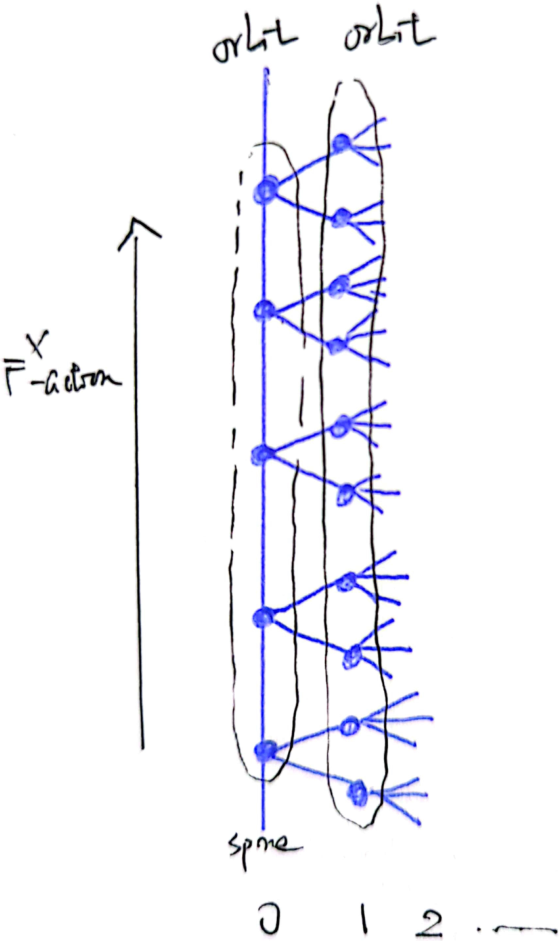
\includegraphics[width=0.33\textwidth]{figures/f91-spinetree.png}
\end{center}

于是 $F^\times$ 按竖直平移作用，而 $X(F)/G(O)$ 中的轨道由到 spine（轴）的距离给出，故
\[
  X(F)/G(O)\cong\mathbb Z_{\ge0}.
\]
因此可以像 $\mathrm{PGL}_2(O)\backslash\mathrm{PGL}_2(F)/\mathrm{PGL}_2(O)$ 的情形那样，把 Hecke 算子写成某些线性递推算子。最终在练习里你会证明
\begin{equation}
  \begin{array}{rcl}
    C_c^\infty(X(F))^{G(O)} & \xrightarrow{\ \sim\ } & \mathbb C[\mathrm{SL}_2/\mathrm{conj}]\\
    \text{基本函数}\ \delta_0=\mathbf 1_{X(O)} & \mapsto & 1\\
    \text{Hecke 算子} & \mapsto & \text{乘算子}\\
    \langle\cdot,\cdot\rangle & \leftrightarrow & \displaystyle\int_{\mathrm{SU}_2(\mathbb R)/\mathrm{conj}}|\cdot|^2\cdot(\check M=T^*\mathbb A^2\ \text{的 q-特征标})\,d_{Haar}.
  \end{array}
  \label{eq:9-1}
\end{equation}
注意 $\mathrm{SL}_2$ 是 $X$ 的对偶群（在此例中等于 $\mathrm{PGL}_2$ 的对偶群），而 $\mathrm{SU}_2=(\mathrm{SL}_2)_c$ 是 $\mathrm{SL}_2$ 的紧形式。稍后我们要做的是把内积与积分几何地重写为几何对象之间 Hom 空间的度量。

\subsection{历史}

不过在此之前，先谈谈匹配问题的历史。回忆对局部域 $F$，有 $A_G(F)=\Rep(G(F))$，而 $\Theta_G(X)=\mathrm{fns}(X(F))$ 是某种函数构成的表示，因此是 $G(F)$ 的表示，即 $\Theta_G(X)\in A_G(F)$。虽然一般局部域上表示论的研究是较晚的事，这类问题（研究 $\Theta_G(X)$ 如何落在 $A_G(F)$ 中）却被考虑了很长时间。

当 $F=\mathbb R$、Lie 群 $G$ 紧、$X$ 是紧 $G$-流形时，这可以追溯到 Cartan（1929）与 Weyl（1934）\footnote{Weyl, H. ``Harmonics on Homogeneous Manifolds.'' \emph{Annals of Mathematics}, vol.\ 35, no.\ 3, 1934, pp.\ 486--99.}。Weyl 与他的学生 Peter 用分析研究紧 Lie 群的表示。他们通过在 $G$ 上构造紧积分算子，证明了 $L^2(G)$ 可以分解为有限维不可约 $G$-表示的直和。后来 Cartan 证明，齐性 $G$-空间 $X$，
\begin{equation}
  L^2(X)\cong\bigoplus_\pi\pi^{m(\pi)},
  \label{eq:9-2}
\end{equation}
其中 $m(\pi)\in\mathbb Z_{\ge0}$ 是 $\pi$ 在 $L^2(X)$ 中的重数。

这个故事与另外两件事相关。第一，分解 (9.2) 与 $X$ 上微分算子的研究密切相关。例如对 $G=\mathrm{SO}_3$、$X=S^2$，这个分解对表示论学家与分析学家都是熟知的。因为它是按 Laplace 算子的本征空间作的分解；该分解给出球调和函数。更一般地，若 $D$ 是 $X$ 上与 $G$-作用交换的微分算子，则 $D$ 在 $L^2(X)$ 中的每个本征空间都是 $G$-表示。最理想的情形是所有重数都不超过 $1$，此时找本征函数与本征值最容易\footnote{而不是去解微分方程。}（由 Schur 引理，$D$ 在每个 $\pi$ 上作为标量作用）。此后许多推广都以此为目标。

与这个分解相关的另一件事是特殊函数的研究。Cartan 证明了当 $X$ 是紧 Riemann 对称空间时 $m(\pi)\le1$。为研究 $\pi$ 如何活在 $L^2(X)$ 中，他通过在 $X\times X$ 上构造 $G$-不变核（等价地，$(X\times X)/G$ 上的函数）来构造投影 $L^2(X)\to L^2(X)_\pi$（$\pi$ 的等类型部分），该核等于带球函数。这一观察很快就推广开了。特别地，到 60 年代 Vilenkin 写了一本书\footnote{Vilenkin, N.~Ja. \emph{Special functions and the theory of group representations}. Translated from the Russian by V.~N.~Singh. Translations of Mathematical Monographs, Vol.\ 22. American Mathematical Society, Providence, RI, 1968. x+613 pp.}，在更一般的设定下讨论此事，其中群 $G$ 不必紧，他研究两个 $G$-空间 $X$ 与 $Y$ 且 $L^2(X)_\pi\cong L^2(Y)_\pi\cong\pi$ 时的 $L^2(X)\to L^2(Y)_\pi$。此时核是 $(X\times Y)/G$ 上的函数。

他的观察是：推广这一进路，可以得到以表示为参数的各种特殊函数，并由此统一地恢复许多经典特殊函数，例如 Bessel 函数、超几何函数等等。

此后 Harish-Chandra 在 50 至 70 年代分类了实半单群 $G$ 的表示，并写出了群情形的 Plancherel 公式，即把 $L^2(G)$ 分解为 $G\times G$-表示，挑出基本函数 $\delta_e$（即 Dirac 测度），并弄清 $\delta_e$ 在分解中的去向。Harish-Chandra 的核心目标是 Plancherel 测度（即研究配对 $(L^2(G),\delta_e)$），而分类是在抵达目标的过程中得到的。从 60 到 70 年代起，人们开始考虑更一般空间的类似问题。其中一部分是研究双曲面上 Laplace 算子的分析学家。多数推广是在对称簇上做的。

2010 年前后，在 Sakellaridis--Venkatesh\footnote{Sakellaridis, Yiannis; Venkatesh, Akshay. \emph{Periods and harmonic analysis on spherical varieties}. Astérisque No.\ 396 (2017), viii+360 pp.} 中，我们提出：研究局部域上 $X$ 的 Plancherel 测度，是研究自守形式的 $X$-周期的局部类比。我们的书把调和分析与人们在自守形式上研究了很久的问题联系起来。与此前各情形一样，重数一假设\footnote{向量空间 $\Hom_G(C_c^\infty(X(F)),\pi)$ 对 $G(F)$ 的任一光滑不可约表示 $\pi$ 至多一维。}起特殊作用，这一点由 Piatetski-Shapiro 强调。这也是我们把范围限制在球簇（更精确地说，超球簇）上的主要原因，因为它们保证重数有限、有时还保证重数一。虽然 BZSV\footnote{D.~Ben-Zvi, Y.~Sakellaridis, A.~Venkatesh, \emph{Relative Langlands Duality}, preprint. 见 \url{https://www.math.ias.edu/~akshay/research/BZSVpaperV1.pdf}。} 非常代数，但手边有 $L^2$ 直觉有助于得到正确的归一化。

\subsection{设定}

假设 (9.1) 成立，并且为简单起见设 $\check G_X=\check G$。例如我们在 $(G,X,\check M)=(\mathrm{GL}_1,\mathbb A^1,T^*\mathbb A^1)$、$(\mathrm{PGL}_2,\mathrm{PGL}_2/\mathbb G_m,T^*\mathbb A^2)$ 见过这一点。

设 $V,W$ 是 $\check G$ 的有限维表示，$\chi_V,\chi_W$ 分别是 $V$ 与 $W$ 的特征标，$T_V,T_W$ 是 Satake 对应所联系的 Hecke 算子。我们要把恒等式
\[
  (T_V\delta_0,T_W\delta_0)=\int_{G^\vee_c}\chi_V(g)\chi_W(g)\cdot(\check M^\vee\ \text{的 q-特征标})\,d_{Haar}g
\]
的两端都几何地重写。左端将解释为 Frobenius 在某个对象 $?$ 上的迹，右端将解释为 q-作用（若 $q=1$ 就是维数）在另一个对象 $??$ 上的迹。这里 $?$ 与 $??$ 都是不同范畴中的 Hom 空间。这将引出我们关于范畴等价的猜想。

\section{第三日第三讲}

本讲第一个目标，是对一个球 $G$-簇 $X$ 联系一个映射
\begin{equation}
  \mathrm{SL}_2\times\check G_X\to\check G.
  \label{eq:10-1}
\end{equation}
这个映射的动机来自对 $H_G$-模 $C_c^\infty(X(F))^{G(O)}$ 的研究：对「好」的 $X$，我们预期有同构
\begin{equation}
  C_c^\infty(X(F))^{G(O)}\cong\mathbb C[\Rep\check G_X].
  \label{eq:10-2}
\end{equation}
它是 $H_G\simeq\mathbb C[\Rep\check G]$ 上的模同构。映射 (10.1) 用来描述这个同构的右端。在解释右端之前，我们先通过定义 $X$ 的 Cartan 子群 $A_X$ 与 Weyl 群 $W_X$，来定义与 $X$ 相联系的嵌入 $\check G_X\hookrightarrow\check G$。

\subsection{相对 Cartan 子群}

设 $B$ 是 $G$ 的 Borel 子群，$X^\circ$ 是相应的开 $B$-轨道。

对 $G$ 可以定义一个环面 $A$，称为 $G$ 的\textbf{万有 Cartan 子群}，使得对任意 Borel 子群 $B$ 连同其幂幺根 $N$，都有典范同构 $B/N\xrightarrow{\sim}A$。由于 $B$ 作用在 $X^\circ$ 上，$A$ 作用在 $X^\circ/N$ 上，而这个作用经过 $A$ 的一个商 $A_X$ 分解。

$A_X$ 的特征群 $X^*(A_X)$ 可以与 $B$-模 $k(X)$ 中出现的 $B$-本征特征标组成的群等同起来。事实上，由于 $X$ 有开稠的 $B$-轨道，$k(X)$ 的 $B$-本征特征标 $\chi\in X^*(B)$ 由相应的非零 $B$-本征函数 $f_\chi\in k(X)^{(B)}$ 决定，而后者在 $k$ 的意义下只差一个标量（即短正合列 (10.3)）。我们还有
\[
  k(X)^{(B)}=k(X^\circ)^{(B)}=k(B_x\backslash B)^{(B)}=k(B_x\backslash B/N)^{(B/N)}=k(X^\circ/N)^{(A)},
\]
其中 $B$-轨道 $X^\circ\simeq B_x\backslash B$，$x\in X^\circ$，$B_x$ 是相应的稳定化子。

在把 $X^*(A_X)$ 等同于 $k(X)$ 的 $B$-本征特征标群之下，我们得到短正合列
\begin{equation}
  1\to k^*\to k(X)^{(B)}\xrightarrow[\ f_\chi\mapsto\chi\ ]{}X^*(A_X)\to 1.
  \label{eq:10-3}
\end{equation}

\subsection{小 Weyl 群}

对一个球 $G$-簇 $X$，小 Weyl 群 $W_X$ 有三种等价的定义/看法。最后一种最便于计算。

\subsubsection{来自 $G$-不变赋值}

设 $V$ 是 $k(X)$ 上 $G$-不变的 $\mathbb Q$-值离散赋值的集合。利用正合列 (10.3)，Knop 证明了有单射
\[
  V\hookrightarrow\Hom(X^*(A_X),\mathbb Q)=X_*(A_X)\otimes\mathbb Q=:\mathfrak a_X,\qquad v\mapsto(f_\chi\mapsto v(f_\chi)).
\]

\begin{prop}
[Knop，见《The Luna--Vust theory of spherical embeddings》]
存在子群 $W_X\subset W$，它稳定 $X^*(A_X)\subset X^*(A)$，并且 $V$ 是 $W_X$ 在 $\mathfrak a_X$ 上作用的基本域。
\end{prop}

\subsubsection{来自余切丛的 GIT 商}

\begin{prop}
[Knop]
设 $X$ 是齐性、拟仿射的球 $G$-簇，$\mathfrak a_X=\mathrm{Lie}\,A_X$，$\mathfrak a=\mathrm{Lie}\,A$，于是 $\mathfrak a_X^*\subset\mathfrak a^*$。存在稳定 $\mathfrak a_X^*$ 的子群 $W_X\subset W$，以及典范同构
\[
  T^*X\gquot G\xrightarrow{\ \sim\ } \mathfrak a_X^*\gquot W_X.
\]
此外，映射 $T^*X\to\mathfrak g^*\to\mathfrak a^*\gquot W$ 经过上述映射分解。
\end{prop}

\begin{exmp}
[群情形]
设 $X=H$，$G=H\times H$ 按 $h\cdot(h_1,h_2)=h_1^{-1}hh_2$ 右作用。则
\[
  T^*H\gquot G=T^*_eH\gquot\mathrm{Stab}_G(e)=\mathfrak h^*\gquot H,
\]
而由 Chevalley 同构 $\mathfrak h^*\gquot H=\mathfrak a_H^*\gquot W_H$，其中 $\mathfrak a_H$ 是 $H$ 中极大环面的 Lie 代数，$W_H$ 是 $H$ 的 Weyl 群。于是 $W_H$ 就是 $X$ 的小 Weyl 群。
\end{exmp}

\subsubsection{来自 Knop 在 Borel 轨道上的 Weyl 群作用}

Knop 在他的论文「On the set of orbits for a Borel subgroup」中定义了 $W_G$ 在 $X$ 的 $B$-轨道上的如下作用：

\begin{defn}
[$W_G$ 在 $X$ 的 $B$-轨道上的作用]
设 $\alpha\in\Delta_G$ 是 $G$ 的单根，$w_\alpha\in W_G$ 是相应的反射。设 $\gamma$ 是 $X$ 中的 $B$-轨道，$P_\alpha\supset B$ 是 $\alpha$ 对应的极小抛物子群，则 $w_\alpha\cdot\gamma$ 将是 $\gamma P_\alpha$ 中的 $B$-轨道，定义如下：$\gamma P_\alpha/R(P_\alpha)$ 是齐性球 $P_\alpha/R(P_\alpha)\simeq\mathrm{PGL}_2$-簇。齐性球 $\mathrm{PGL}_2$-簇在等价意义下只有 $4$ 种类型，我们用下表在每种类型的 Borel 轨道上定义 $w_\alpha$ 的作用：

\smallskip
\noindent\begin{tabular}{|c|c|p{0.30\textwidth}|}
  \hline
  类型 & 齐性球 $\mathrm{PGL}_2$-簇 & Borel 轨道与 $w_\alpha$ 的作用\\
  \hline
  $G$ & $\mathrm{pt}$ & 一个闭轨道\\
  \hline
  $T$ & $\mathbb G_m\backslash\mathrm{PGL}_2$ & 两个闭轨道、一个开轨道；$w_\alpha$ 交换两个闭轨道、不动开轨道\\
  \hline
  $N$ & $N(\mathbb G_m)\backslash\mathrm{PGL}_2$ & 一个闭轨道、一个开轨道；$w_\alpha$ 不动这两个轨道\\
  \hline
  $U$ & $N\cdot S\backslash\mathrm{PGL}_2$，其中 $N=\begin{pmatrix}1&a\\0&1\end{pmatrix}\subset S\subset B$ & 一个开轨道、一个闭轨道；$w_\alpha$ 交换这两个轨道\\
  \hline
\end{tabular}
\smallskip

合起来，这就定义了 $G$ 的 Weyl 群 $W_G$ 在 $X$ 的 $B$-轨道上的一个作用。
% [Tutor Note: 原文 U 行写作 "one open and open closed orbit"，词序有误；按上下文（$w_\alpha$ 交换两个轨道）应为「一个开轨道、一个闭轨道」，译文按此理解，已在 reports/ch10.md 登记。]
\end{defn}

\begin{defn}
给定球 $G$-簇 $X$，可以联系一个抛物子群 $P(X):=\{g\in G\mid X^\circ g=X^\circ\}$ 连同其 Levi 子群 $L(X)$。若 $P(X)=B$，则称 $X$ 是\textbf{tempered} 的。
\end{defn}

\begin{exmp}
[tempered 性]
群情形是 tempered 的。
\end{exmp}

小 Weyl 群在 Knop 的作用之下这样出现：

\begin{prop}
[Knop]
在此作用下，开 $B$-轨道 $X^\circ$ 的稳定化子是
\[
  W_X\ltimes W_{P(X)},
\]
其中 $W_{P(X)}$ 是 $P(X)$ 的 Weyl 群。
\end{prop}

我们将用这个命题来计算某些 $X$ 的小 Weyl 群。

\begin{exmp}
[群情形]
设 $X=H$，$G=H\times H$ 按 $h\cdot(h_1,h_2)=h_1^{-1}hh_2$ 右作用。另一种看法是把 $X$ 看作 $X=H_{\mathrm{diag}}\backslash H\times H$，而 $G=H\times H$ 按右乘作用。

由 Bruhat 分解，$X$ 的 $B\times B$-轨道是 $BwB$（$w\in W_H$），其中 $W_H$ 是 $H$ 的 Weyl 群。开 $B\times B$-轨道是 $Bw_0B$，其中 $w_0\in W_H$ 是由 $B\subset H$ 定义的最长元素。

对 $H\times H$ 的单根 $(\alpha,0)\in\Delta_{H\times H}=\Delta_H\sqcup\Delta_H$，相应的极小抛物子群是 $P_\alpha\times B$。考虑
\[
  (Bw_0B)\cdot(P_\alpha\times B)/R(P_\alpha\times B)=R(P_\alpha)\backslash P_\alpha w_0B/B.
\]
这总是类型 $U$\footnote{可以证明 $R(P_\alpha)w_0B\in R(P_\alpha)\backslash P_\alpha w_0B/B$ 在 $R(P_\alpha)\backslash P_\alpha$ 作用下的稳定化子是 $R(P_\alpha)\backslash B^-\cap P_\alpha$，因此有同构
  $\mathrm{PGL}_2/B^-\xrightarrow{\sim}R(P_\alpha)\backslash P_\alpha/(B^-\cap P_\alpha)\xrightarrow{[g]\mapsto[gw_0]}R(P_\alpha)\backslash P_\alpha w_0B/B$。}（见上表）。特别地，我们知道
$w_{(\alpha,0)}=(w_\alpha,1)\in W_{H\times H}=W_H\times W_H$ 在 $P_\alpha w_0B$ 中交换哪两个 Borel 轨道。事实上，由于 $P_\alpha=B\sqcup Bw_\alpha B$ 且 $w_0(\alpha)\in\Phi^-$，故\footnote{见 Tits 系统下 Bruhat 分解的证明。}
\[
  P_\alpha w_0B=Bw_0B\sqcup Bw_\alpha w_0B.
\]
类似地，$w_{(0,\alpha)}=(1,w_\alpha)\in W_{H\times H}=W_H\times W_H$ 交换 $Bw_0B$ 与 $Bw_0w_\alpha B=Bw_\alpha w_0B$（因为对任意 $w\in W$、$\alpha\in\Phi$ 有 $ww_\alpha w^{-1}=w_{w(\alpha)}$）。这说明 $(w_\alpha,w_\alpha)$ 不动开 Borel 轨道 $X^\circ=Bw_0B$。此外，$(w,w')\in W_{H\times H}$ 不动 $X^\circ$ 当且仅当 $w=w'$。由于 $X$ 是 tempered 的，$W_{P(X)}=1$，于是由 Knop 的作用得到 $W_X=\{(w,w):w\in W_H\}$。
\end{exmp}

\begin{exmp}
[$X=\mathrm{PGL}_2^{\mathrm{diag}}\backslash\mathrm{PGL}_2^3$ 作为 $\mathrm{PGL}_2^3$-空间]
记 $B$ 为 $\mathrm{PGL}_2$ 中的上三角矩阵。先计算 $X$ 的开 Borel 轨道，即 $\mathrm{PGL}_2^{\mathrm{diag}}\backslash\mathrm{PGL}_2^3/B^3$ 中最大的双陪集。把 $\mathrm{PGL}_2^3/B^3$ 与 $(\mathbb P^1)^3$ 等同，容易看出最大轨道对应于代表元 $x=([1,0],[0,1],[1,1])\in(\mathbb P^1)^3$：因为 $\mathrm{PGL}_2$ 在 $\mathbb P^1$ 上可迁地作用，要得到大轨道就需要三个互不相同的点。

先通过计算稳定化子 $B_x$ 来求 $A_X$。等同 $\mathrm{PGL}_2/B$ 与 $\mathbb P^1$ 由
\[
  \begin{pmatrix}a&*\\c&*\end{pmatrix}\leftrightarrow[a,c]
\]
给出。于是经过一些矩阵乘法（注意这里 $B^3$ 从右作用），可以看出 $B_x=\{1\}$，从而 $A_X=\mathbb G_m^3$。

现在计算 $W_X$。对 $(1,1,w)$（$w$ 是 $W_{\mathrm{PGL}_2}$ 中的非平凡元素），相应的极小抛物子群是 $B\times B\times\mathrm{PGL}_2$。取 $x$ 在 $\mathrm{PGL}_2^3$ 中的一个代表元，计算商
\[
  \begin{aligned}
    Y_2&=\mathrm{PGL}_2^{\mathrm{diag}}\Big\backslash\Big(\begin{pmatrix}1&0\\0&1\end{pmatrix}B,\ \begin{pmatrix}0&1\\1&0\end{pmatrix}B,\ \begin{pmatrix}1&0\\1&1\end{pmatrix}B\Big)\cdot B\times B\times\mathrm{PGL}_2\,/\,B\times B\times\{1\}\\
    &=\mathrm{PGL}_2^{\mathrm{diag}}\backslash B\times wB\times\mathrm{PGL}_2\,/\,B\times B\times\{1\}\\
    &\cong\mathrm{PGL}_2\backslash\mathrm{PGL}_2=\text{点}.
  \end{aligned}
\]
因此 $(1,1,w)$ 稳定开 Borel 轨道。另两个单根的情形类似。可以验证与 $X$ 相联系的抛物子群是 $B^3$，从而 $W_X=W_{\mathrm{PGL}_2^3}$。
\end{exmp}

\begin{exmp}
[练习中的其他例子]\leavevmode\par
\begin{enumerate}[label=(\arabic*),leftmargin=1.8em,itemsep=0.2em]
  \item $X=\mathrm{Mat}_n$ 作为 $\mathrm{GL}_n\times\mathrm{GL}_n$-空间。
  \item $X=\mathrm{SO}_n\backslash\mathrm{SO}_{n+1}$ 作为 $\mathrm{SO}_{n+1}$-空间。
  \item $X=\mathrm{SO}_{n+1}$ 作为 $\mathrm{SO}_n\times\mathrm{SO}_{n+1}$-空间。预期答案：$\check G_X=\check G$。
\end{enumerate}
\end{exmp}

\subsection{球簇的对偶群}

对偶群 $\check G_X$ 看作 $\check G$ 的子群，由它的 Cartan 子群 $A_X$ 与 Weyl 群 $W_X$ 完全确定。

\begin{exmp}
[群情形]
当 $X=H$、$G=H\times H$ 时，可以证明 $\check G_X=\check H$。
\end{exmp}

\begin{exmp}
当 $X=\mathrm{PGL}_2^{\mathrm{diag}}\backslash\mathrm{PGL}_2^3$ 时，$\check G_X=\check G$。
\end{exmp}

\begin{exmp}
[Hecke]
当 $X=\mathbb G_m\backslash\mathrm{PGL}_2$ 时……
\end{exmp}

\subsection{$\mathrm{SL}_2$-项}

见 BZSV，§4。

我们已经定义了 $i:\check G_X\to\check G$。由此 $\mathbb C[\Rep\check G_X]$ 是 $\mathbb C[\Rep\check G]$ 上的模，其中 $V\in\Rep\check G$ 通过 $i^*V\otimes W$ 作用在 $W\in\Rep\check G_X$ 上。然而这并非给出 (10.2) 的正确模结构。需要对 $i$ 作一个移位，下面的例子说明这一点。

\begin{exmp}
[Whittaker]
设 $X=\mathrm{pt}=G\backslash G$。$H_G$ 通过平凡特征标 $\chi_1:H_G\to\mathbb C$ 作用在 $C_c^\infty(X(F))^{G(O)}=\mathbb C$ 上。在 Satake 同构 $\Hom(H_G,\mathbb C)=(\check A\gquot W)(\mathbb C)$ 之下，$\chi_1$ 对应于 $q^\rho\in\check A(\mathbb C)$。

如何解释这个 $q^\rho$：$\rho\in\check{\mathfrak g}$ 对应于 $\rho=d\tilde\rho$，其中 $\tilde\rho:\mathbb G_m\to\check G$，而 $q^\rho=\tilde\rho(q)$。

可以对 $X$ 联系一个 $\mathfrak{sl}_2$-三元组 $(h,e,f)$，它在 $\check L(X)\subset\check G$（$P(X)\subset G$ 对应的 Levi 子群）中是主三元组。这个三元组与 $\check G_X$ 交换，从而定义 $\iota:q^{h/2}\check G_X\hookrightarrow\check G$，它提升为 $\mathrm{SL}_2\times\check G_X\to\check G$。$i$ 的这个移位 $\iota$ 给出 (10.2)。
\end{exmp}

\begin{exmp}
[Whittaker]
验证这个移位在作用的意义下是正确的。$\mathfrak{sl}_2$-三元组 $(h,e,f)$ 是主三元组，其中 $P(X)=\cdots$
\end{exmp}

\subsection{超球簇}

本讲第二个目标是推广球簇。由此引出超球簇的概念。基本的例子是球簇的余切空间。

\begin{defn}
带交换 $G_{\mathrm{gr}}$ 的 Hamilton $G$-簇 $M$ 称为\textbf{超球}的，若它满足下列条件：
\begin{enumerate}[label=(\arabic*),leftmargin=1.8em,itemsep=0.15em]
  \item $M$ 光滑且仿射。
  \item 作为 $G$-簇，$M$ 是余迷向的。
  \item $G$ 在 $M$ 上作用的通常稳定化子连通。
  \item 矩映射 $M\to\mathfrak g^*$ 的像与幂零锥相交（即交非空）。
  \item 分次作用是「中性的」。特别地，它与 $\mathfrak g^*$ 上的平方作用相容。
\end{enumerate}
\end{defn}

\begin{rem}\leavevmode\par
\begin{itemize}[leftmargin=1.4em]
  \item 关于 (4)：若 $M=T^*X$，则矩映射的像总包含零截面。
  \item 实验表明 (2)+(3) 与 (1) 对偶。
\end{itemize}
\end{rem}

\begin{exmp}
[$M$ 不是 $T^*X$ 形状的情形]
考虑 $T^*(N\backslash G)$，其中 $N$ 是 $B$ 的幂幺根。我们用 Hamilton 约化来解释商空间的余切空间，其定义为矩映射下 $\{0\}$ 的纤维对 $N$ 的商：
\[
  T^*(N\backslash G)\overset{\text{def}}{=}N\gquot G=\{0\}\times_N\mathfrak n^*T^*G.
\]
也就是说，我们看的是 $G$ 上与 $N$-轨道正交的余切向量。注意这个空间不是仿射的。

略作修改即得 Whittaker 余切空间。构造它时，先取 $\mathfrak g\simeq\mathfrak g^*$ 中的 $\mathfrak{sl}_2$-三元组 $(h,e,f)$。我们要 $f$ 在 $\mathfrak g^*$ 中正则幂零，使 $f$ 给出 $\mathfrak n$ 的非退化特征标。令 Whittaker 余切空间为
\[
  T^*((N,f)\backslash G)=\{f\}\times_N\mathfrak n^*T^*G=M.
\]
这样 $M$ 是仿射的，且是超球的。注意它还带有 Kostant 截面
\[
  M\gquot G=\mathfrak a^*\gquot W\xrightarrow{\ \text{Kostant}\ }M.
\]
这给出 $M\simeq(\mathfrak a^*\gquot W)\times G$。
\end{exmp}

\begin{thm}
[超球簇的结构定理]
超球 Hamilton $G$-簇 $M$ 由下列数据搭成：
\[
  (G,H,\iota,S),
\]
其中 $G$ 是约化群，$H$ 是 $G$ 的约化子群，$\iota$ 是 $G$ 中的一个 $\mathfrak{sl}_2$-三元组，$S$ 是 $G$ 的辛表示。
\end{thm}

上述构造称为 Whittaker 诱导，记作 $M=\mathrm{W}_\iota\mathrm{Ind}_H^G(S)$。

对这样的空间 $M$，我们期待某个对偶空间 $\check M$。

当 $M=T^*X$（$X$ 球簇）时，我们有如下对应
\[
  \check M\ \longleftrightarrow\ (\check G,\check G_X,\iota_{P(X)},\check S),
\]
其中 $\check G$ 是对偶群，$\check G_X$ 是此前定义的与 $X$ 相联系的约化子群，$\iota_{P(X)}$ 是 $P(X)$ 对应的 $\mathfrak{sl}_2$-三元组，$\check S$ 是由 $X$ 的颜色（即非 $G$-稳定的 $B$-稳定除子）决定的辛 $\check G$-表示（在同构意义下）。非典范地有
\[
  \check M\simeq V_X\times_{\check G_X}\check G,\qquad V_X=\check S\oplus(\check{\mathfrak g}/\check{\mathfrak g}_X)_e+\check{\mathfrak g}_1,
\]
其中 $e$ 来自 $\mathfrak{sl}_2$-三元组 $\iota_{P(X)}$，而 $\check{\mathfrak g}_1$ 是 $\check{\mathfrak g}$ 中的 $1$ 次部分。

对任意 $\mathfrak{sl}_2$-三元组 $\iota:\mathfrak{sl}_2\hookrightarrow\mathfrak g$，$h$ 通过 $[h,-]$ 的本征值给出 $\mathfrak g$ 的分次
\[
  \mathfrak g=\mathfrak g_+\oplus\mathfrak g_0\oplus\mathfrak g_-,
\]
其中总有 $f\in\mathfrak g_{-2}$。若这个 $\mathfrak{sl}_2$-三元组给出偶分解（即只有偶次），则在等同 $\mathfrak g\simeq\mathfrak g^*$ 下，$f$ 定义一个特征标 $f:\mathfrak g_+\to F$。一般情形下，$f$ 定义一个特征标 $\mathfrak g_{\ge2}\times\mathfrak g_{\ge2}\to F$（Heisenberg 群）。

\section{第四日第一讲（Akshay）}

\subsection{Plancherel 公式}

回忆我们有两个 TQFT：$A_G$ 与 $B_{\check G}$。取 $Y:=\mathbb F_q((t))$，我们期待一个 2-范畴的等价 $A_G(Y)\to B_{\check G}(Y)$。给定球 $G$-簇 $X$ 带来的额外数据，我们有相应的边界理论 $\Theta_{G,X}\in A_G(Y)$ 与 $\Theta_{\check G,\check X}\in B_{\check G}(Y)$。我们期待这两个 1-范畴也等价。

先分析我们想要的等价在去范畴化之后的版本。取 $F=\mathbb F_q((t))$、$O=\mathbb F_q[[t]]$，设 $X$ 是球 $G$-簇。在某些有限性假设下，我们有
\begin{equation}
  C_c(X(F))^{G(O)}\cong\mathbb C[\Rep\check G_X]
  \label{eq:11-1}
\end{equation}
其中 $\check G_X\subset\check G$ 是某个群。就本讲而言，我们设 $\check G_X=\check G$（这就是 BZSV 里所谓的 \textbf{strongly tempered} 条件）。上述同构不仅是 $H(G(F),G(O))\cong\mathbb C[\Rep\check G]$ 的模同构，它还保持内积。设 $f,g\in C_c(X(F))^{G(O)}$，$\hat f,\hat g$ 是它们在 (11.1) 下的像，则
\begin{equation}
  \langle f,g\rangle=\int_{\check G_c}\langle\hat f,\hat g\rangle\cdot\mathrm{q\text{-}char}(\check G\times G_{gr}^m,M^\vee)\,d\mu_H.
  \label{eq:11-2}
\end{equation}
记号说明如下：

\begin{itemize}[leftmargin=1.6em]
  \item $\check G_c$ 是复约化群 $\check G$ 的紧形式。
  \item $M^\vee$ 是某个带 $\check G\times G_{gr}^m$ 作用的空间，通常是 $T^*\check X$。
  \item $M^\vee$ 上的 q-特征标，指的是把 $\mathbb C[M^\vee]$ 看作 $\check G\times G_{gr}^m$ 的表示所得的 q-特征标。
  \item $\mu_H$ 是 Haar 测度。
\end{itemize}

在同构 (11.1) 下，示性函数 $\mathbf 1_{X(O)}$ 应当被送到平凡表示。

\begin{exmp}
我们已对下面两个情形算过 Plancherel 公式：
\begin{enumerate}[label=(\arabic*),leftmargin=1.8em]
  \item $G=\mathbb G_m$，$X=\mathbb A^1$。此时 $\check G=\mathbb G_m$，$M^\vee=T^*\mathbb A^1$。
  \item $G=\mathrm{PGL}_2$，$X=\mathrm{PGL}_2/\mathbb G_m$。此时 $\check G=\mathrm{SL}_2$，$M^\vee=T^*\mathbb A^2$。
\end{enumerate}
\end{exmp}

\subsection{内积作为 Hom 空间上的迹}

一个关键的观察是：(11.2) 的两端都可以实现为某些算子在某个 Hom 空间上的迹。设 $\hat f=\chi_V$（表示 $V$ 的特征标），$\hat g=\chi_W$。换句话说，$f=h_V*\mathbf 1_{X(O)}$，$g=h_W*\mathbf 1_{X(O)}$。为简单起见，我们把 (11.2) 的左端记作 LHS，右端记作 RHS。

注意若 $A,B$ 是 $\check G$ 的复表示，则 $\chi_A\chi_B$ 是 $\Hom(B,A)$ 的特征标，故
\begin{equation}
  \int_{\check G_c}\chi_A\chi_B\,d\mu_H=\dim\Hom(B,A)^{\check G}=\dim\Hom_{\check G}(B,A).
  \label{eq:11-4}
\end{equation}
于是
\begin{align}
  \mathrm{RHS}&=\int_{\check G_c}\chi_V\chi_W\Big(\sum_i q^{-\frac i2}\chi_{\mathbb C[M^\vee]_i}\Big)d\mu_H
  \label{eq:11-5}\\
  &=\sum_i q^{-\frac i2}\dim\Hom_{\check G}(W,V\otimes\mathbb C[M^\vee]_i)\,d\mu_H
  \label{eq:11-6}\\
  &=\operatorname{tr}\Big(q^{-\frac12},\Hom_{\check G}(W,V\otimes\mathbb C[M^\vee])\Big).
  \label{eq:11-7}
\end{align}
在这些等式中，我们把 $q^{-\frac12}$ 看作 $G_{gr}^m(\mathbb C)=\mathbb C^\times$ 中的元素。

现在把 $\mathbb C$-线性映射 $W\to V\otimes\mathbb C[M^\vee]$ 看作 $\mathbb C[M^\vee]$-线性映射 $W\otimes\mathbb C[M^\vee]\to V\otimes\mathbb C[M^\vee]$，可以得到一个更对称的表述。于是
\begin{equation}
  \mathrm{RHS}=\operatorname{tr}\Big(q^{-\frac12},\Hom_{\check G,\mathbb C[M^\vee]}(W\otimes\mathbb C[M^\vee],V\otimes\mathbb C[M^\vee])\Big).
  \label{eq:11-8}
\end{equation}
令 $\mathcal V=V\otimes\mathbb C[M^\vee]$。它是一个 $O(M^\vee)$-模，带 $\check G$ 作用，因此可以看作 $M^\vee/\check G$ 上的凝聚层。类似地定义 $\mathcal W$。于是
\begin{equation}
  \mathrm{RHS}=\operatorname{tr}\Big(q^{-\frac12},\Hom_{M^\vee/\check G}(\mathcal W,\mathcal V)\Big).
  \label{eq:11-9}
\end{equation}
这里的 $\Hom$ 是在 $M^\vee/\check G$ 上拟凝聚层（indcoherent？）的导出范畴中取的。

(11.2) 的左端可以用层-函数对应实现为迹。回忆一个一般事实：设 $Z$ 是 $\mathbb F_q$ 上的簇，$F,G$ 是 $Z_{\mathbb F_q}$ 上的混合 $\bar{\mathbb Q}_\ell$-层，则取 Frobenius 的迹得到 $Z(\mathbb F_q)$ 上的函数 $f,g$。我们有
\begin{equation}
  \operatorname{tr}\Big(\mathrm{Fr}^{-1}\,\Big|\,\Hom_{Z_{\mathbb F_q}}(F,G)\Big)=\sum_{z\in Z(\mathbb F_q)}f(z)g(z).
  \label{eq:11-10}
\end{equation}
注意这里的 $g$ 是 $DG$ 的迹（$G$ 的 Verdier 对偶）。例如取 $F=DG=\bar{\mathbb Q}_{\ell,Z}$（$Z$ 上的常值层），上式就化归 Lefschetz 不动点公式。

现在取 $F=\mathbb F_q((t))$、$O=\mathbb F_q[[t]]$。对很多定义在 $\mathbb F_q$ 上的「好」$X$，$X(F)/G(O)$ 是某个「合理的代数栈」$X_F/G_O$ 的 $\mathbb F_q$-点。例如当 $X=H$、$G=H\times H$ 时，$X(F)/G(O)$ 就是仿射 Grassmann 流形 $\mathrm{Gr}_G$ 的 $\mathbb F_q$-点，而它是一个 ind-scheme。

Hecke 代数 $H_G$ 在 $C_c(X(F))^{G(O)}$ 上的作用，可以升级为 Hecke 范畴在 $X_F/G_O$ 上的层的作用。这里的 Hecke 范畴是 $\mathrm{Gr}_G$ 上 $G(O)$-等变可构造混合 $\bar{\mathbb Q}_\ell$-层的导出范畴。记 $\mathrm{IC}_V$ 为几何 Satake 同构下与表示 $V$ 对应的反常层。令 $\delta_0:=j_*(\bar{\mathbb Q}_{\ell,X_O/G_O})$，其中 $j:X_O/G_O\to X_F/G_O$ 是闭嵌入（？）。则在层-函数对应下，LHS 中的 $f,g$ 分别是与 $\mathrm{IC}_W*\delta_0$ 与 $\mathrm{IC}_V*\delta_0$ 相联系的函数。

于是可以写
\begin{equation}
  \mathrm{LHS}=\operatorname{tr}\Big(\mathrm{Fr}^{-1}\,\Big|\,\Hom(\mathrm{IC}_W*\delta_0,\mathrm{IC}_V*\delta_0)\Big).
  \label{eq:11-11}
\end{equation}
这里的 $\Hom$ 在 $X_F/G_O$ 上可构造层的范畴中取值。

\subsection{局部猜想}

上一节的讨论强烈提示一个范畴等价（并不正确，尚需修正）：
\begin{equation}
  \mathrm{Shc}(X_F/G_O)\cong\QCoh(M^\vee/\check G).
  \label{eq:11-12}
\end{equation}
该等价应当满足：

\begin{itemize}[leftmargin=1.6em]
  \item $\delta_0$ 应被送到 $M^\vee/\check G$ 上的结构层 $\mathcal O$。
  \item 左端的 Frobenius 作用应当对应右端 $q^{\frac12}\in G_{gr}^m$ 的作用。
  \item 该等价与 Hecke 范畴的模结构相容（在导出 Satake 同构之下）。在 Abel 范畴的层面，$H_G$ 从左端以卷积作用，$\Rep(\check G)$ 从右端以张量积作用：对 $\check G$ 的任意表示 $V$，沿 $M^\vee/\check G\to*/\check G$ 拉回可得 $M^\vee/\check G$ 上的向量丛，$V$ 的作用就是与该向量丛作张量积。
\end{itemize}

该等价可以看作把 (11.1) 开头讨论的边界条件匹配起来。

上面这个等价按原样并不正确。在说修正之前，先做一点合理性检验。若该等价成立，则应当有同构
\begin{equation}
  \Hom_{\mathrm{Shc}(X_F/G_O)}(\delta_0,\delta_0)\cong\Hom_{M^\vee/\check G}(\mathcal O,\mathcal O).
  \label{eq:11-13}
\end{equation}
左端等于 $H^*(X_O/G_O)$。注意 $G_O/G$ 是 pro-unipotent 的，因此可缩，对上同调没有贡献。类似地 $X_O$ 收缩到 $X(\mathbb F_q)$。于是
\begin{equation}
  H^*(X_O/G_O)\cong H^*_G(X(\mathbb C)).
  \label{eq:11-14}
\end{equation}
右端则有
\begin{equation}
  \Hom_{\QCoh(M^\vee/\check G)}(\mathcal O,\mathcal O)\cong\mathbb C[M^\vee]^{\check G}.
  \label{eq:11-15}
\end{equation}
所以我们应当检验
\begin{equation}
  H^*_G(X(\mathbb C))=\mathbb C[M^\vee]^{\check G}.
  \label{eq:11-16}
\end{equation}

\begin{exmp}
考虑 $G=\mathbb G_m$、$X=\mathbb A^1$、$\check G=\mathbb G_m$、$M^\vee=T^*\mathbb A^1$ 的情形。此时 $H^*_G(X)=\mathbb C[\xi^2]$，其中 $\xi^2$ 位于同调次数 $2$。回忆 $\lambda\in\check G$ 作用在 $(x,y)\in T^*\mathbb A^1$ 上为 $(\lambda x,\lambda^{-1}y)$。我们有 $\mathbb C[M^\vee]^{\check G}=\mathbb C[xy]$。
\end{exmp}

\begin{exmp}
考虑 $G=\mathrm{PGL}_2$、$X=\mathrm{PGL}_2/\mathbb G_m$、$\check G=\mathrm{SL}_2$、$M^\vee=T^*\mathbb A^2$ 的情形。此时 $H^*_G(X)=H^*_{\mathbb G_m}(\mathrm{pt})=\mathbb C[\xi^2]$。另一方面，把 $M^\vee=T^*\mathbb A^2$ 实现出来，$\mathrm{SL}_2$ 以左乘作用，则有 $\mathbb C[M^\vee]^{\check G}=\mathbb C[\det]$。
\end{exmp}

两个例子中都验证了代数同构，但还得给右端配上正确的分次。在范畴层面有一个称为 \textbf{shearing} 的步骤，修正后的猜想如下：
\begin{equation}
  \mathrm{Shc}(X_F/G_O)\cong\IndCoh(M^\vee/\check G)^\natural.
  \label{eq:11-19}
\end{equation}

\section{第四日第二讲}

在这节轻松的讲次里，我们转到整体情形，并给出一些动机与历史。我们先补上上一讲没来得及讲完的一件事：沿着我们已经走过的推理，甚至可以得到一般的无分歧 Plancherel 公式。

设 $F$ 是局部域。「数据包」$(C_c^\infty(X_F)^{G_O},\delta_e,\langle-,-\rangle)$ 于是可以完全用对偶的 $\check M$ 来描述，也就是说，Hecke 作用可以对角化。我们在一处轻微的简化假设下描述答案，即假设 $\check M$ 总形如 $\check G\times_{\check G_X}V_X$（$V_X$ 是某个 $\check G_X$-表示），且其上的 $\mathbb G_m$-作用完全来自 $V_X$ 上的作用。此时有同构
\[
  C_c^\infty(X_F)^{G_O}\overset{\sim}{\longrightarrow}\mathbb C[\check G_X]^{\check G_X},
\]
它把 $\delta_e$ 送到常函数 $1$，并把内积 $\langle-,-\rangle$ 送到积分
\[
  \langle-,-\rangle\mapsto\int_{\check G_{X,\mathrm{compact}}}\langle-,-\rangle\cdot(\text{$V_X$ 的 q-特征标})\cdot d_{Haar}.
\]
回忆 Haar 测度与 $V_X$ 的 q-特征标之积称为 Plancherel 测度。

局部情形到此为止；现在转到整体情形。我们的两个理论 $A_G$ 与 $B_{\check G}$ 将在算术流形上取值，其中 $Y$ 要么是 $\mathbb F_q$ 上的曲线，要么是代数闭包 $\overline{\mathbb F}_q$ 上的曲线。前一种情形 $A_G(Y)$ 与 $B_{\check G}(Y)$ 都是向量空间；后一种情形两者都是范畴。$G\circlearrowleft X$ 与 $\check G\circlearrowleft\check X$ 的数据（真正应当想的是 $M$ 与 $\check M$ 的数据）定义了对象 $\Theta_{G,X}\in A_G(Y)$ 与 $\Theta_{\check G,\check X}\in B_{\check G}(Y)$。本讲只专注于定义 $\Theta_{G,X}\in A_G(Y)$。（一切在数域情形同样成立，但为方便起见我们只讲函数域情形。）

我们有 $\mathbb F_q$ 上的曲线 $\Sigma$，向量空间 $A_G(\Sigma)$ 是 $G$-丛的集合 $[G]$ 上的函数空间。这些 $G$-丛定义在 $\mathbb F_q$ 上。$G$-丛集合 $[G]$ 既可以用阿代尔方式理解，也可以用几何方式理解。设 $K$ 是 $\Sigma$ 的函数域，则 $[G]$ 可以写成 $G(K)\backslash G(\mathbb A)/G(\hat O)$；$[G]$ 的点记作 $[g]$，而对每个闭点 $s\in\Sigma$，记 $g_s\in G(\hat O_s)$ 为相应的元素。

周期函数 $\Theta_{G,X}\in A_G(\Sigma)$ 可以用三种不同方式定义。

\begin{itemize}[leftmargin=1.6em]
  \item 几何方式：$\Theta_{G,X}([g])$ 是与 $[g]$ 相伴的 $X$-丛的截面个数。回忆这个 $X$-丛就是 $(X\times[g])/G$。
  \item $\Theta_{G,X}([g])$ 是满足下述条件的截面 $x\in X(K)$ 的个数：对一切闭点 $s\in\Sigma$，截面 $xg_s$ 属于 $X(\hat O_s)$。要看出这与第一条的数量相同，注意把这个 $X$-丛限制到曲线的泛点就得到 $X$（因为丛局部平凡）；于是与 $[g]$ 相伴的 $X$-丛的截面在一般纤维上就是一个点 $x\in X(K)$。要求该截面整体有定义，等价于要求 $x$ 在 $\Sigma$ 的任何闭点处都没有极点，即 $x\in X(\hat O_s)$。
  \item 算术方式：$\Theta_{G,X}([g])$ 是求和 $\sum_{x\in X(K)}\Phi(x\cdot g)$，其中 $\Phi$ 是 $\prod X(\hat O_s)$ 在 $X(\mathbb A)$ 中的示性函数。
\end{itemize}

下面算几个例子。取 $\Sigma=\mathbb P^1$、$G=\mathbb G_m$。此时 $\mathbb P^1$ 上的 $\mathbb G_m$-丛只由一个整数确定（即 $n$ 对应 $\mathcal O(n)$），故 $[G]=\mathbb Z$。再取 $X=\mathbb A^1$。取相伴的 $X$-丛无非是取该线丛的全空间，于是 $\Theta_{G,X}=:\Theta_X$ 把 $n$ 送到 $\mathcal O(n)$ 的整体截面个数。换句话说：
\[
  \Theta_X(n)=\begin{cases}q^{n+1},& n\ge0,\\ 1,& n\le-1.\end{cases}
\]
一个重要的注记是：在我们那篇论文里，需要对周期函数作正确的归一化。所以我们其实用的是周期函数的一个轻微变体，在这个例子里就是把上面的函数 $\Theta_X$ 乘上因子 $q^{-n/2}$。于是这个重标定把
\[
  n\mapsto\begin{cases}q^{n/2+1},& n\ge0,\\ q^{-n/2},& n\le-1.\end{cases}
\]
注意现在它关于 $n=-1$ 对称。（周期函数的这个归一化是由 $L^2$-理论驱动的。）

再做一个例子。设取定子群 $H\subseteq G$。此时可以取 $X=G/H$，并考虑 $\Theta_X:=\Theta_{G,X}$ 与某个函数 $f:[G]\to\mathbb C$ 的「配对」。（当 $G=\mathrm{PGL}_2$、$H=\mathbb G_m$ 时，这个配对在 1930 年代由 Hecke 算出。）所谓「配对」指的是：

\begin{itemize}[leftmargin=1.6em]
  \item 用阿代尔均匀化表述，是积分 $\int_{G(K)\backslash G(\mathbb A)}\Theta_X(g)f(g)\,dg$。这里取 Haar 测度使 $G(\hat O)$ 的体积为 $1$。
  \item 用几何图景表述，是求和 $\sum_{[g]\in[G]}\frac{1}{\#\mathrm{Aut}([g])}\Theta_X(g)f(g)$。例如在 $\mathbb G_m$ 情形，点 $[\mathcal O(n)]$ 的测度是 $1/\#\mathbb G_m(\mathbb F_q)=1/(q-1)$。
\end{itemize}

两者给出同一个数。一个好练习是验证：当 $X=G/H$ 时，这两个配对都可以用 $H$ 改写。即
\[
  \sum_{[g]\in[G]}\frac{1}{\#\mathrm{Aut}([g])}\Theta_X(g)f(g)=\sum_{[h]\in[H]}\frac{1}{\#\mathrm{Aut}([h])}f(h),
\]
\[
  \int_{G(K)\backslash G(\mathbb A)}\Theta_X(g)f(g)\,dg=\int_{[H]}f(h)\,dh,
\]
而且这些数全都相等，给出 $\langle\Theta_X,f\rangle$。这是个有帮助的练习。

下面我们来看这类配对 $\langle\Theta_X,f\rangle$ 的研究史，以及数论学家最初为何对它们感兴趣。为此一直回溯到 Riemann zeta 函数 $\zeta(s)=\sum_{n=1}^\infty n^{-s}$。它有三条性质，合起来极其刚性：

\begin{itemize}[leftmargin=1.6em]
  \item 它有 Euler 积 $\prod_p(1-p^{-s})^{-1}$。
  \item 它有解析（指亚纯）延拓。
  \item 它有函数方程，联系 $s$ 与 $1-s$ 处的值。
\end{itemize}

一个函数要同时具备这三条性质并不容易；我们就把这类函数称作「L-函数」。人们开始发现这样的 L-函数，而它们全都与算术有关：与 Dirichlet 特征标、数域、Galois 表示相联系，后来又与椭圆曲线相联系。但要证明这些函数具备上述全部性质却很难！重要的是，所有这类（预期的）L-函数都与算术本性的对象有关。

Hecke 就在这时登场了，大约是 1936 年。他发现了一种完全不同的办法，从全纯模形式（它们是如今所谓 Hecke 算子的本征函数）产生这类函数。即给定 $f(q)=\sum a_nq^n$，可以写下 L-函数 $L(f,s)=\sum a_nn^{-s}$。有 Euler 积这条性质可追溯到 Ramanujan，而它有解析延拓与函数方程的证明归功于 Hecke。他知道 Riemann 证明 zeta 函数函数方程时用到了 $\theta$-函数，这很可能是给他的重要动机。Hecke 的关键观察是：若把全纯模形式 $f$ 看作自守形式 $f:[\mathrm{PGL}_2]\to\mathbb C$，则
\[
  \int_{[\mathbb G_m]}f(h)|h|^s\,dh=L(f,s).
\]
不必在意此式中的特征标 $|h|^s$；撇开这一点，它就是 $f$ 与周期函数 $\Theta_{\mathrm{PGL}_2,\mathrm{PGL}_2/\mathbb G_m}$ 的配对。这很了不起，因为它是这类 L-函数的一个解析的（而非算术的）来源。

Hecke 之后，人们开始发现其他几种用分析方法产生 L-函数的途径。下一个例子属于 1940 年代的 Rankin 与 Selberg。他们从一对 Hecke 本征形式 $f,g$ 产生 L-函数。若写 $f(q)=\sum a_nq^n$、$g(q)=\sum b_nq^n$，则 Rankin–Selberg L-函数是 $\sum_{n\ge1}\frac{a_n\bar b_n}{n^s}$。它有 Euler 积并不太难，但它的解析延拓或函数方程则完全不显然。他们证明这些的方式，用我们的语言来说，就是把 $f\boxtimes g$（看作 $G=\mathrm{GL}_2\times\mathrm{GL}_2$ 的自守形式）与 $\Theta_{G,X}$ 配对，其中 $X=\mathrm{GL}_2\times\mathbb A^2$。这里 $\mathrm{GL}_2$ 的两个因子分别从左、右作用在 $\mathrm{GL}_2$ 上，而只有第二个 $\mathrm{GL}_2$ 作用在 $\mathbb A^2$ 上。Rankin 的动机并不是研究素数，他感兴趣的是估计 $|a_n|$。这个证明非常重要，因为它为 Deligne 证明 Weil 猜想时用到的某些关键不等式提供了启发。

此后有一段时间没有更多例子。但 Godement 与 Jacquet 在 1970 年前后，从 $\mathrm{GL}_n$ 上的 Hecke 本征形式 $f$ 出发生成了 L-函数。他们同样是靠证明该 L-函数由 $f$ 与 $\Theta_{G,X}$ 配对给出（其中 $G=\mathrm{GL}_n\times\mathrm{GL}_n$、$X=\mathrm{Mat}_n$）来证明它有解析延拓与函数方程。在所有这些论文里，你能看到的是积分以及对它们的操作；把这件事概念化为「研究某个空间」要晚得多。此后自守形式理论兴起，上述情形被大量推广。

1960 年代前后，Langlands 猜想所有 L-函数（包括所有算术 L-函数）都来自自守形式。这很重要，因为来自自守形式的 L-函数有很多例子和工具可用，而算术 L-函数几乎什么都没有。这成为发展自守形式 L-函数理论的极强动机。

我们要强调，Hecke、Rankin–Selberg、Godement–Jacquet 等人的所有这些例子都有下述形式。考虑配对 $\langle f,\Theta_{G,X}\rangle$，结果要么是 $0$，要么给出一个与 $f$ 相关的 L-函数。而配对 $\langle f,\Theta_{G,X}\rangle$ 非零的条件，恰好由对偶 Hamilton $\check G$-空间 $\check M$ 打包得很好。更详细地说，这个配对是否消没与对偶群 $\check G_X$ 有关；而配对非零时得到的 L-函数则与 $V_X$ 有关，也就是 Plancherel 测度里出现的那个表示。此外，$\Theta_{G,X}$ 只依赖余切丛 $M=T^*X$。所以大量例子由一对 $(M,\check M)$ 打包。

然而，并非所有已知例子都落在超球对偶的框架内。这是这类例子中最漂亮的一类，但最好能对框架作某种推广。

\section{第五日第一讲}

\subsection{回顾}

回忆我们想要在种种设定（整体算术、整体几何、局部算术、局部几何）下等同两个理论，即（$G$ 的）自守理论与（$\check G$ 的）谱理论。特别地，边界理论（例如 L-函数与周期）应当匹配。举例来说，Fargues--Scholze 关于算术局部域（如 $\mathbb Q_p$）上局部 Langlands 对应的表述，与曲线上几何 Langlands 有相似之处。

在局部算术设定中，回忆 $C_c^\infty(X_G)^{G_O}$ 对应对偶空间 $\check M$ 及其上的 $\check G$ 作用。把它范畴化，就得到局部几何猜想，它联系
\[
  \Shv(X_F/G_O)\cong\QCoh(\check M/\check G).
\]

\begin{exmp}
对群情形，即 $G\times G$ 作用在 $X=G$ 上，在对偶侧有 $\check G\times\check G$ 作用在 $\check X=\check G$ 上，于是 $\check M=T^*\check G\cong\check G\times\check{\mathfrak g}^*$。局部几何猜想此时还原为导出几何 Satake 等价：A 侧是 $\Shv(G_O\backslash G_F/G_O)$，B 侧是 $\QCoh(\check{\mathfrak g}^*/\check G)$。B 侧经 Koszul 对偶与 TQFT 在 raviolo 上的赋值等同。更精确地说，我们有
\[
  B_{\check G}\Big(D\coprod_{D^\times}D\Big)=\QCoh^!(\check{\mathfrak g}[-1]/\check G)\cong\QCoh(\check{\mathfrak g}^*/\check G).
\]
这里第一个恒等式来自 TQFT 的场描述，最后一个等价是 Koszul 对偶。
\end{exmp}

今天的目标是讨论整体几何猜想，然后理解把整体几何猜想与局部几何猜想、整体算术猜想联系起来的那些箭头。

\subsection{设定}

固定 $\Sigma$ 为 $\mathbb C$ 或 $\mathbb F_q$ 上光滑射影代数曲线。

有群 $G$ 作用在 $X$ 上，我们给它配上周期层 $P_X\in\Shv(\Bun_G\Sigma)$。对偶地，$\check G$ 作用在 $\check X$ 上，我们给它配上 L-层 $L_{\check X}\in\QCoh^!(\Loc_{\check G}\Sigma)$。无分歧几何 Langlands 匹配这两个范畴，而相对 Langlands 进一步匹配对象，也就是说，周期层应当匹配 L-层。

\begin{rem}
相对朗兰兹对偶给出的对象匹配，比几何 Langlands 对应的表述与证明中所用的多得多。
\end{rem}

\subsection{$\Bun^X_G$ 与周期层}

考虑 $\Bun^X_G=\Bun^X_G(\Sigma)=\Maps(\Sigma,X/G)$，它是分类「$\Sigma$ 上的 $G$-丛连同相伴 $X$-丛的截面」的栈。这个栈带有一个自然的映射
\setcounter{equation}{2}
\begin{equation}
  \pi:\ \Bun^X_G\to\Bun_G.
  \label{eq:13-3}
\end{equation}
% [Tutor Note: 原文的 (13.1)(13.2) 编号在印刷本中未出现（节内计数器却已进两位），译本按印刷面保留无编号显示，并把计数器置为 2，使 (13.3) 之后的编号与原文一致。]

\begin{defn}
我们由公式
\[
  P_X:=\pi_!\,k_{\Bun^X_G}
\]
定义周期层。
\end{defn}

\begin{exmp}
取 $G=\mathbb G_m$，则
\[
  \Bun_G=\Pic_\Sigma\cong\mathbb Z\times\Jac_\Sigma\times B\mathbb G_m.
\]
\end{exmp}

\begin{exmp}
考虑 $\Bun_{\mathrm{SL}_2}(\mathbb P^1)$。它不紧。它是连通的，其点对应 $\mathcal O\oplus\mathcal O$、$\mathcal O(1)\oplus\mathcal O(-1)$、……。它们被赋予这样的拓扑：当 $0\le b\le a$ 时，$\mathcal O(a)\oplus\mathcal O(-a)$ 落在 $\mathcal O(b)\oplus\mathcal O(-b)$ 的闭包中。
\end{exmp}

\subsection{局部系}

与 $\Bun_G$ 对偶地，我们考虑
\begin{equation}
  \Loc^{\check X}_{\check G}\Sigma:=\Maps_{k\text{-}l.c.}(\Sigma,\check X/\check G),
  \label{eq:13-7}
\end{equation}
它带有一个映射
\begin{equation}
  \check\pi:\ \Loc^{\check X}_{\check G}\Sigma\to\Loc_{\check G}\Sigma:=\Maps_{k\text{-}l.c.}(\Sigma,\mathrm{pt}/\check G),
  \label{eq:13-8}
\end{equation}
其中下标 $k\text{-}l.c.$ 表示局部常值映射。

\begin{exmp}
对 $G=\mathbb G_m$，有
\begin{equation}
  \Loc_{\check G}=B\mathbb G_m\times(\mathbb G_m)^{2g}\times(\text{导出部分}),
  \label{eq:13-10}
\end{equation}
其中 $g$ 是 $\Sigma$ 的亏格。更典范地说，因子 $(\mathbb G_m)^{2g}$ 可以看作 $H^1(\Sigma,\mathbb C^\times)$。
\end{exmp}

\subsection{L-层及其纤维}

我们对 $\check G$-空间 $\check X$ 定义相应的 L-层，并研究它的纤维。回忆我们有映射 $\check\pi:\Loc^{\check X}_{\check G}\to\Loc_{\check G}$。

\begin{defn}
我们由公式
\[
  L_{\check X}:=\check\pi_*\,\omega_{\Loc^{\check X}_{\check G}}\in\QC^!(\Loc_{\check G})
\]
定义 L-层。
\end{defn}

\begin{rem}
层 $\omega_{\Loc^{\check X}_{\check G}}$ 与 $\mathcal O_{\Loc^{\check X}_{\check G}}$ 之间有同构。
\end{rem}

\begin{rem}
为什么要用对偶化层而不是结构层？大致是因为范畴 $\IndCoh$ 偏爱对偶化层，而范畴 $\QCoh$ 偏爱结构层。
\end{rem}

\begin{rem}
我们得对 L-层作归一化，它在函数层面相当于对 L-函数作归一化，以使内积有意义。
\end{rem}

给定局部系 $E\in\Loc_{\check G}$，$\check\pi$ 在 $E$ 处的纤维有如下几种等价描述：

\begin{enumerate}[label=(\arabic*),leftmargin=1.8em]
  \item $E$ 的相伴 $\check X$-丛的局部常值截面；
  \item 被 $E$ 扭的局部常值映射 $\Sigma\to\check X$；
  \item $\check X$ 上 $\pi_1(\Sigma)$ 的不动点。
\end{enumerate}

在最后一种描述里，我们用的是 $\pi_1(\Sigma)$ 经由 $E:\pi_1(\Sigma)\to\check G$ 拉回 $\check G$ 在 $\check X$ 上的作用而得到的作用。事实上，上述所有描述都应在导出意义下理解。把 $\check\pi$ 在 $E$ 处的纤维记作 $\check\pi^{-1}E$。

\begin{rem}
人们会问：给定群 $H$ 作用在空间 $Y$ 上，它的导出不动点轨迹是什么意思？经典地，不动点轨迹可以解释为从 $\mathrm{pt}/H$ 到 $Y$ 的映射空间。我们通过考虑从 $\mathrm{pt}/H$ 到 $Y$ 的导出映射空间来理解导出不动点轨迹。
\end{rem}

由定义，给定局部系 $E$，$L_{\check X}$ 在 $E$ 处的纤维是 $R\Gamma(\check\pi^{-1}E,\omega)$。因此 $L_{\check X}$ 在「$R\Gamma(\check\pi^{-1}E,\omega)$ 有限维」的轨迹上是凝聚的；等价地，在（经典）不动点个数有限处凝聚。这也可以说成（经典）不动点孤立。

\begin{exmp}
设 $\check X$ 是 $\check G$ 的线性表示。不动点孤立等价于 $\pi_1\Sigma$ 在 $\check X$ 上没有平凡子表示。这个条件决定了 $\Loc_{\check G}$ 上使 L-层 $L_{\check X}$ 凝聚的轨迹。
\end{exmp}

\subsection{整体几何猜想}

现在我们陈述 BZSV 的整体几何猜想。先陈述一个朴素版本。

\begin{conj}[朴素整体几何猜想]
周期层 $P_X$ 与 L-层 $L_{\check X}$ 在几何 Langlands 对应下匹配：
\[
  \mathbb L_G:\ \Shv(\Bun_G)\to\QC^!(\Loc_{\check G}),\qquad P_X\mapsto L_{\check X}.
\]
\end{conj}

回忆 A 侧有三种层论可供选择，即 de Rham、Betti 与 étale。除 de Rham 设定外，这个猜想应当作修改：对几何 Langlands 对应的陈述而言，A 侧的层应当满足某个条件 $N$。从 TQFT 的角度看这是自然的。由 TQFT 的局部常值公理，Hecke 范畴（即 $A_G(D_x\coprod_{D_x^\times}D_x)$）在 $\Bun_G$ 上层范畴（即 $A(\Sigma)$）上的作用，应当在 $x\in\Sigma(F)$ 上局部常值。并非所有 $\Bun_G$ 上的层都满足这一要求，因此我们应当替换 A 侧，考虑子范畴 $\Shv_N(\Bun_G)$，使这种局部常值性成立。于是 Betti 或 étale 设定下修改后的几何 Langlands 对应陈述是一个等价
\[
  \mathbb L_G:\ \Shv_N(\Bun_G)\to\QC^!(\Loc_{\check G}).
\]

\begin{rem}
在 de Rham 设定中不需要条件 $N$，因为每个 D-模都在较弱的意义下局部常值。
\end{rem}

下面两个 $G=\mathbb G_m$ 的例子从两个角度说明条件 $N$ 的必要性。两个例子都在 Betti 设定下工作。

\begin{exmp}[TQFT]
令 $G=\mathbb G_m$。我们有 $\Bun_G=\Pic$。给定 $n\in\mathbb Z$ 与点 $x\in\Sigma(F)$，有自同构
\[
  m_x^n:\ \Pic\to\Pic,\qquad \mathcal L\mapsto\mathcal L(nx).
\]
把 $\Rep\mathbb G_m^\vee$ 的权 $n$ 表示看作点 $x\in\Sigma(F)$ 处球 Hecke 范畴中的对象。该对象在 $\Shv(\Pic)$ 上的作用等同于 $(m_x^n)^*:\Shv(\Pic)\to\Shv(\Pic)$。空间 $\Pic$ 有 $\mathbb Z$ 个分支，按次数标号；由 Hecke 作用的局部常值条件可知，$F\in A_G(\Sigma)$ 应当在每条分支上局部常值。
\end{exmp}

\begin{exmp}[直接计算]
回忆 $\Pic=\Jac\times(\cdots)$、$\Loc_{\mathbb G_m}=H^1(\Sigma,\mathbb C^\times)\times(\cdots)$，其中 $(\cdots)$ 是某些额外因子。为简单起见，把两侧的额外因子都丢掉。我们有
\[
  \QCoh(H^1(\Sigma,\mathbb C^\times))=O(H^1(\Sigma,\mathbb C^\times))\text{-}\mathrm{Mod}.
\]
Fourier 变换给出同构 $O(H^1(\Sigma,\mathbb C^\times))\cong\mathbb C[H_1(\Sigma,\mathbb Z)]$，右端应理解为群代数。于是得到
\[
  \QCoh(\Loc_{\mathbb G_m})\cong H_1(\Sigma,\mathbb Z)\text{-}\mathrm{Mod}.
\]
另一方面 $H_1(\Sigma,\mathbb Z)=\pi_1(\Jac)$，于是我们确认了等价
\[
  \Loc(\Jac)\cong\QCoh(\Loc_{\mathbb G_m}).
\]
由此可以断定：几何 Langlands 对应迫使 A 侧的层局部常值。这与上一个例子的结论一致。
\end{exmp}

到此我们已经修改了几何 Langlands 对应。要陈述 BZSV 猜想还得再作一处修改，因为周期层不一定属于范畴 $\Shv_N(\Bun_G)$。不过我们有 Beilinson 投影 $(-)_{\mathrm{spec}}:\Shv(\Bun_G)\twoheadrightarrow\Shv_N(\Bun_G)$，于是可以期待下面这一点。

\begin{conj}[整体几何猜想]
周期层 $P_X$ 的投影与 L-层 $L_{\check X}$ 在几何 Langlands 对应下匹配：
\[
  \mathbb L_G:\ \Shv_N(\Bun_G)\to\QC^!(\Loc_{\check G}),\qquad (P_X)_{\mathrm{spec}}\mapsto L_{\check X}.
\]
\end{conj}

\begin{rem}
我们忽略了一些技术问题，例如归一化与对偶对合。该猜想更精确的形式见 BZSV 的猜想 12.1.1。
\end{rem}

\subsection{关于 Beilinson 投影}

为说明 Beilinson 投影对周期层的必要性，我们来看周期层与 L-层的一些例子。

\begin{exmp}
令 $X=\mathrm{pt}$，我们称此情形为 Neumann 边界条件。此时映射 $\pi:\Bun^X_G\to\Bun_G$ 是恒等，故 $P_{\mathrm{pt}}=k_{\Bun_G}$。若令 $\check X=\mathrm{pt}$，同样地 $L_{\mathrm{pt}}=\omega_{\Loc_{\check G}}$。注意 $\omega_{\Loc_{\check G}}$ 有来自 $\Loc_{\check G}$ 的辛结构的平凡化。这个辛结构用 $\mathfrak g^\vee$ 的 Killing 型典范地定义。
\end{exmp}

\begin{exmp}
若取 $G$-空间 $X=G$，我们称此情形为 Dirichlet 边界条件。此时映射 $\pi:\Bun^X_G\to\Bun_G$ 是平凡丛处的包含 $\mathrm{pt}\hookrightarrow\Bun_G$。于是 $P_G$ 是平凡丛处的摩天楼层。同样地，$L_{\check G}$ 是平凡局部系处的摩天楼层。
\end{exmp}

\begin{rem}
若 $G$ 交换，这两个例子经 Fourier 变换互为对偶。
\end{rem}

在例 13.24 中，周期层 $P_G$ 是摩天楼层，因而远非局部常值。这告诉我们周期层不一定住在范畴 $\Shv_N(\Bun_G)$ 里，从而说明了 Beilinson 投影的必要性。

\begin{rem}
L-层一般并不落在范畴 $\IndCoh_{\mathrm{Nilp}}(\Loc_{\check G})$ 中。注意我们用的是「更大」版本的几何 Langlands 对应，允许 B 侧上一切 ind-凝聚层。
\end{rem}

条件 $N$ 与 Beilinson 投影看起来像是整体几何猜想的讨厌特征。不过我们关心的 $\Shv_N$ 中的测量可以通过伴随提升为 $\Shv$ 中的测量。投影 $(-)_{\mathrm{spec}}:\Shv(\Bun_G)\twoheadrightarrow\Shv_N(\Bun_G)$ 与包含 $\Shv_N(\Bun_G)\hookrightarrow\Shv(\Bun_G)$ 之间有伴随。在 Betti 设定中，投影左伴随于包含；在 étale 设定中，投影右伴随于包含。用这个伴随，在 Betti 设定中有
\begin{equation}
  \Hom_{\Shv_N}((P_X)_{\mathrm{spec}},F)=\Hom_{\Shv}(P_X,F)
  \label{eq:13-27}
\end{equation}
其中 $P_X$ 是周期层，$F$ 是 Hecke 特征层。若把 $\Hom$ 空间反过来看，étale 设定也有类似陈述。注意在数论中，周期与自守函数之间的配对才是我们在 A 侧主要关心的测量。因此数论感觉不到范畴 $\Shv$ 与 $\Shv_N$ 的差别。

我们用一个简单例子结束对 Beilinson 投影的讨论。

\begin{exmp}
回忆例 13.24 中 $P_G=i_!k$，其中 $i:\mathrm{pt}\hookrightarrow\Bun_G$ 是平凡丛处的包含。如前所述，它不满足条件 $N$，因而需要投影到范畴 $\Shv_N$。思路是把 $\mathrm{pt}$ 换成一个同伦等价的空间 $C$（即可缩空间），以便沿映射 $j:C\to\Bun_G$ 取 $!$-推前。若选取的替换 $C$ 使 $C\to\Bun_G$ 是纤维化，则层 $j_!k_C$ 局部常值，因而落在 $\Shv_N$ 中。我们令 $(P_G)_{\mathrm{spec}}=j_!k_C$。
\end{exmp}

\subsection{Iwasawa--Tate 情形的合理性检验}

相对朗兰兹对偶最重要的例子之一是 Iwasawa--Tate 情形，即 $G=\mathbb G_m$ 作用在 $X=\mathbb A^1$ 上，$\check G=\mathbb G_m$ 作用在 $\check X=\mathbb A^1$ 上。该情形下猜想 13.21 的证明由 Feng--Wang 的 \emph{Geometric Langlands duality for periods} 定理 6.1.2 给出。我们不重复其证明，而是通过比较两侧的 $\Hom$ 空间作一个简单的合理性检验。本小节只在 Betti 设定下工作。这一检验更详细的叙述见 BZSV 第 12.2.3 节。

设 $E$ 是 $\Sigma$ 上非平凡的 $\mathbb G_m$-局部系，它确定 $\QC^!(\Pic)$ 中的摩天楼层 $C_E$。在几何 Langlands 对应下，它对应 $\Pic$ 上的一个秩一 $\mathbb C$-线性局部系 $F_E$。局部系 $F_E$ 有如下性质：对每个 $r\ge0$，它在映射
\[
  \phi_r:\ \Sigma_r\to\Pic,\qquad (P_1,\cdots,P_r)\mapsto\mathcal O(P_1+\cdots+P_r)
\]
下的拉回是 $E^{\boxtimes r}$。这里 $E$ 也用来记与它相伴的秩一 $\mathbb C$-线性局部系。于是猜想 13.21 预言
\[
  \Hom_{\Shv_N}((P_{\mathbb A^1})_{\mathrm{spec}},F_E)\cong\Hom_{\QC^!(\Loc_{\mathbb G_m})}(L_{\mathbb A^1},C_E).
\]
由伴随 (13.27)，它等价于
\begin{equation}
  \Hom_{\Shv}(P_{\mathbb A^1},F_E)\cong\Hom_{\QC^!(\Pic)}(L_{\mathbb A^1},C_E).
  \label{eq:13-29}
\end{equation}
下面给出此式的证明。

由伴随，(13.29) 的右端是 $L_{\mathbb A^1}$ 在 $E$ 处纤维的对偶。如 13.5 小节所述，$L_{\mathbb A^1}$ 在 $E$ 处的纤维是 $R\Gamma(\check\pi^{-1}E,\omega)$，其中 $\check\pi^{-1}E$ 是 $\pi_1(\Sigma)$ 作用在 $\mathbb A^1$ 上的导出不动点轨迹。由注 13.12，对偶化层的导出截面与 $\check\pi^{-1}E$ 的函数代数等同。合起来得到
\begin{equation}
  \Hom_{\QC^!(\Pic)}(L_{\mathbb A^1},C_E)\cong O(\check\pi^{-1}E)^*.
  \label{eq:13-30}
\end{equation}
由于我们假设 $E$ 非平凡，导出栈 $\check\pi^{-1}E$ 只有一个经典点，即零截面。于是它的函数代数由切复形决定。切复形是 $H^1(\Sigma,E)[-1]$，故
\begin{equation}
  O(\check\pi^{-1}E)=\Sym(H^1(\Sigma,E)^*[1]).
  \label{eq:13-31}
\end{equation}
结合 (13.30) 与 (13.31) 得到
\begin{equation}
  \Hom_{\QC^!(\Loc_{\mathbb G_m})}(L_{\mathbb A^1},C_E)\cong\Sym(H^1(\Sigma,E)[-1]).
  \label{eq:13-32}
\end{equation}

现在计算 (13.29) 的左端。映射 $\check\pi:\Bun^{\mathbb A^1}_{\mathbb G_m}\to\Pic$ 有一个截面 $i:\Pic\to\Bun^{\mathbb A^1}_{\mathbb G_m}$，相当于选取相伴 $\mathbb A^1$-丛的零截面。截面 $i$ 是闭嵌入，于是可以考虑补开浸入
\[
  j:\ \Bun^{\mathbb A^1,0}_{\mathbb G_m}\to\Bun^{\mathbb A^1}_{\mathbb G_m}.
\]
注意开子栈 $\Bun^{\mathbb A^1,0}_{\mathbb G_m}$ 分类的是一对 $(L,s)$，其中 $L$ 是 $\Sigma$ 上的线丛、$s$ 是它的非平凡截面。按重数取截面的零点，这个栈等同于有效除子的栈 $\Sym\Sigma$。于是我们有正合三角
\begin{equation}
  C_{\Pic}\to P_{\mathbb A^1}\to j_!C_{\Sym\Sigma}.
  \label{eq:13-33}
\end{equation}
我们断言 $\Hom_{\Shv}(C_{\Pic},F_E)=0$。

回忆 $\Pic$ 由按 $\mathbb Z$ 编号的多份 $\Jac\times B\mathbb G_m$ 组成（例 13.5），而 Hecke 算子置换这些拷贝（例 13.19）。由于局部系 $F_E$ 是非平凡的 Hecke 特征层，上述事实告诉我们 $F_E$ 在每份 $\Jac\times B\mathbb G_m$ 上都非平凡。于是为证明该断言，只需证明：对 $\Jac\times B\mathbb G_m$ 上任何非平凡秩一局部系 $F$，有 $\Hom_{\Jac\times B\mathbb G_m}(C_{\Jac\times B\mathbb G_m},F)=0$。这等价于 $F$ 的单值表示的群上同调的一个消没陈述。由于 $\Jac$ 是环面，该断言由下述事实推出：对有限秩自由交换群 $\Lambda$ 及其非平凡特征 $k_\chi$，群上同调群 $H^*(\Lambda,k_\chi)$ 消没。

把该断言与正合三角 (13.33) 结合，得到
\[
  \Hom_{\Shv}(P_{\mathbb A^1},F_E)\cong\Hom_{\Shv}(j_!C_{\Sym\Sigma},F_E).
\]
用伴随以及 $j$ 是开浸入这一事实，可改写为
\begin{equation}
  \Hom_{\Shv}(P_{\mathbb A^1},F_E)\cong R\Gamma(\Sym\Sigma,j^*F_E).
  \label{eq:13-34}
\end{equation}
回忆 $F_E$ 经 $\phi_r:\Sigma_r\to\Pic$ 拉回为 $E^{\boxtimes r}$，故
\[
  R\Gamma(\Sigma_r,\phi_r^*F_E)=R\Gamma(\Sigma,E)^{\otimes r}=(H^1(\Sigma,E)[-1])^{\otimes r}.
\]
由此可以期待
\[
  R\Gamma(\Sym\Sigma,j^*F_E)\cong\Sym(H^1(\Sigma,E)[-1]).
\]
这与 (13.34) 结合即给出
\begin{equation}
  \Hom_{\Shv}(P_{\mathbb A^1},F_E)\cong\Sym(H^1(\Sigma,E)[-1]).
  \label{eq:13-35}
\end{equation}
比较 (13.32) 与 (13.35)，我们通过了合理性检验 (13.29)。

\section{第五日第二讲}

\textbf{免责声明}：我尽力忠实复现这场报告，但对可能引入的任何不确切或遗漏表示歉意。特别是，我发现自己很难复现那些只是口头说出、并未写下的内容。

\textbf{记号说明}：为了把不同记录人的笔记合成一份统一的讲义，我将用 $(-)^{\mathrm{sh}}$ 表示 BZSV 中 shearing（「斜框」）的记号。注意这个记号的含义在报告中并未精确定义，只是大致说过：它把非零的上同调次数转成 $\mathbb G_m$-分次。

\begin{conj}
\footnote{下面这个猜想（粗略版本）在报告中并未完整写出，其中的 $L$ 是我按自己的理解补上的。}
在几何 Langlands 对应下
\[
  \begin{array}{rcl}
    \Shv(\Bun_G)&\xrightarrow{\ (-)_{\mathrm{spec}}\ }&\Shv_N(\Bun_G)\simeq\QC^!(\Loc_{\check G}),\\[2pt]
    P&\mapsto&L.
  \end{array}
\]
对涉及 $\Hom$ 的问题，
\[
  \Hom(P_{\mathrm{spec}},\text{Hecke 特征层})=\Hom(P,\text{「自守形式」})
\]
对上面的谱投影 $(-)_{\mathrm{spec}}$ 不敏感。
\end{conj}

此外还有
\[
  \begin{array}{rcl}
    \bigotimes_{s\in S}\Shv(X_F/G_O)&\xrightarrow{\ \Theta\ }&\Shv(\Bun_G(\Sigma)),\\[2pt]
    \delta_0:=k_{X_O/G_O}\ (\text{基本对象})&\mapsto&P_X=\Theta(\delta_0)\ (\text{周期层}).
  \end{array}
\]
上面的映射与两侧 $H$ 的作用都相容。

在函数层面：
\[
  \begin{array}{rcl}
    C_c^\infty(X_F/G_O)&\xrightarrow{\ \Theta\ }&\Fun(\{\text{在 }s\text{ 处带平凡化的 }G\text{-丛}\})\ni P=\Theta(\delta_0).
  \end{array}
\]

上述内容有一个全分歧版本（下面两行中标出的 $G_F$ 在两侧同时作用）：
\[
  \begin{array}{rcl}
    \Shv(X_F)&\to&\Shv(\Bun_{G,s}),\qquad G_F\text{ 在两侧作用},\\[2pt]
    C_c^\infty(X_F)&\xrightarrow{\ \Theta\ }&\Fun(\Bun_G(\mathbb F_q)),\qquad G_F\text{ 在两侧作用}.
  \end{array}
\]

在极化情形 $\check M=T^*\check X$，我们如下定义相应的 L-层：
\[
  \begin{array}{rcl}
    \QC_{\mathrm{sh}}(\check M/\check G)&\to&\QC^!(\Loc_{\check G}\Sigma),\\[2pt]
    \mathcal O&\mapsto&L_{\check X}.
  \end{array}
\]
注意左端等价于 $\QC^!(\Loc^{\check X}_{\check G}(\text{去心圆盘}))$，而上面 $\mathcal O$ 对应的对象是对偶化层 $\omega$。

\begin{exmp}
$G\circlearrowleft G/H=X$，$X/G=\bullet/H$，
\[
  \Bun_H=\Bun^X_G\xrightarrow{\ \pi\ }\Bun_G,\qquad P_{G/H}=\pi_!k_{\Bun_H},
\]
\[
  \Hom(P_{G/H},F)=\Gamma(\Bun_H,\pi_!F),\qquad P_H(f)=\int_{[H]}f\big|_{[H]},
\]
其中 $f$ 是 $[G]$ 上的自守形式。
\end{exmp}

\begin{exmp}
$G\circlearrowleft G/N=X\circlearrowleft T$，$X/(G\times T)=\bullet/B$，
\[
  \Bun^X_{G\times T}=\Bun_B\ \longrightarrow\ \Bun_G,\qquad \Bun_T.
\]
由这个对应得到 Eisenstein 级数函子
\[
  \mathrm{Eis}:\ \Shv(\Bun_T)\rightleftarrows\Shv(\Bun_G):\ \text{常项（Constant Term）}.
\]
它是由 $P_{G\circlearrowleft G/N\circlearrowleft T}$ 表示的积分变换。这里的对偶是
\[
  G\circlearrowleft G/N\circlearrowleft T\quad\Longleftrightarrow\quad\check G\circlearrowleft\check G/\check N\circlearrowleft\check T
\]
以及
\[
  \begin{array}{ccc}
    \Shv(\Bun_G)&\longleftrightarrow&\QC^!(\Loc_{\check G})\\
    \updownarrow&&\updownarrow\\
    \Shv(\Bun_T)&\longleftrightarrow&\QC^!(\Loc_{\check T})\\[2pt]
    \Bun_B&&\Loc_{\check B}.
  \end{array}
\]
\end{exmp}

\begin{rem}
周期层与 Hecke 特征层相距甚远。在谱侧，这大致就是摩天楼层与 L-层之间的差别。
\end{rem}

\begin{exmp}[群情形]
球簇
\[
  G\times G\circlearrowleft G\quad\Longleftrightarrow\quad\check G\times\check G\circlearrowleft\check G\quad(\text{模去 Chevalley 扭})
\]
对应下列边界条件：
\[
  G\ \big|^{\mathrm{id}}G\ \longrightarrow\ \check G\ \big|^{\mathrm{id}}\check G
\]
以及
\[
  \begin{array}{c}
    \Bun^{X=G}_{G\times G}\simeq\Bun_G\\[1pt]
    {\scriptstyle\Delta}\big\downarrow\\[1pt]
    \Bun_G\times\Bun_G=\Bun_{G\times G}
  \end{array}
\]
其中 $\Delta$ 是对角嵌入，且
\[
  P_{\mathrm{group}}=\Delta_!k,\qquad L_{\mathrm{group}}=\Delta_!\omega.
\]
这编码了 Gaitsgory 的 Miraculous Duality，它说 $\Shv(\Bun_G)$ 有一个版本的 Verdier 对偶，与谱侧的 Serre 对偶相匹配。
\end{exmp}

\begin{exmp}
\[
  \mathbb G_m\circlearrowleft\bullet\ (\text{Neumann})\quad\Longleftrightarrow\quad\mathbb G_m\circlearrowleft\mathbb G_m\ (\text{Dirichlet}).
\]
右端 $\mathbb G_m$ 在 $\mathbb G_m$ 上的作用是（左）乘法\footnote{补充：当然，由于 $\mathbb G_m$ 交换，左乘右乘没有区别。}，而这是一个非球簇的例子。
\end{exmp}

\begin{exmp}
$M=T^*G/\!/_f\check N\circlearrowleft G$（$f\in\mathfrak n^*$），$G\circlearrowleft\bullet$，
\[
  P_\bullet=k_{\Bun_G}\quad\longleftrightarrow\quad L_{\mathrm{Whit}}\ (\text{谱 Whittaker 层}).
\]
Whittaker 归一化：
\[
  P_{\mathrm{Whit}}\quad\longleftrightarrow\quad L_\bullet=\mathcal O_{\Loc_{\check G}}=\omega_{\Loc_{\check G}},
\]
\[
  \Hom(L_\bullet,-)=R\Gamma(\Loc_{\check G},-),\qquad \Hom(P_{\mathrm{Whit}},-)=R\Gamma(\Bun_N,\text{对某个特征标}).
\]
\end{exmp}

\begin{exmp}\footnote{补充：注意下面 $\underline{\mathrm{Gr}}_G$ 带下划线，指的不是仿射 Grassmann 流形 $\mathrm{Gr}_G$，而是 Hecke 栈 $G_O\backslash G_F/G_O$。}
$\Sigma=$「raviolo」$=D\sqcup_{D^*}\!D$。此时
\[
  P_\bullet=k_{\underline{\mathrm{Gr}}_G},\qquad \Hom(P_\bullet,-)=H^*(\underline{\mathrm{Gr}}_G,-)=H^*_{G(O)}(\mathrm{Gr}_G,-),
\]
以及
\[
  c=\mathfrak g/\!/\check G=\mathfrak h/\!/W\simeq\check{\mathfrak h}^*/\!/W,
\]
\[
  \Shv(\Bun_G(\text{raviolo}))\ \leftrightarrow\ \QC_{\mathrm{sh}}(\check{\mathfrak g}^*/\check G),\qquad
  H^*_G(\bullet)\text{-}\mathrm{Mod}=\mathbb C[\check G]\text{-}\mathrm{Mod}\ \simeq\ K^*.
\]
（回到 Whittaker 情形）有
\[
  \check G\backslash T^*\check G/\!/_f\check N\xrightarrow{\ \mu\ }\check G\backslash\check{\mathfrak g}^*\simeq\check G\backslash(\check G\times c).
\]
$\mathfrak{sl}_2^*$ 的情形的图示：Kostant 截面 $\kappa$ 是特征多项式映射 $\check{\mathfrak g}^*/\check G\to c$ 的截面，由 $f+Z\mathfrak g(e)$ 给出。Hitchin 截面是 Kostant 切片的整体类比，它与整体幂零锥横截相交。Whittaker 层就是 Hitchin 截面上的常值层。
\[
  T^*\Bun_G=\Maps\Big(\Sigma,\frac{\mathfrak g^*}{G}\Big/\!_{G_m}\times\Omega^1\Big)\to\Maps\Big(\Sigma,\frac{c}{G_m}\times\Omega^1\Big).
\]
Gaiotto 拉格朗日（子流形）是一个自然态射的像：它由矩映射（模去 $G$）$\mu:M/G\to\mathfrak g^*/G$ 诱导，
\[
  \Bun^M_G=\Maps(\Sigma,M/G)\to\Maps(\Sigma,\mathfrak g^*/G).
\]
\end{exmp}

\section{第五日第三讲}

Ben-Zvi 已经解释了：当把曲线放到 $\overline{\mathbb F}_q$ 上时，有 $\theta_{G,X}\leftrightarrow\theta_{\check G,\check X}$。

本讲我想回到 $\mathbb F$ 上曲线 $\Sigma$ 的情形，说明形如
\begin{equation}
  \langle P_X,f\rangle=\begin{cases}0,&\text{某些情形},\\ \text{某个 L-函数},&\text{其余情形}\end{cases}
  \label{eq:15-1}
\end{equation}
的公式可以写成与 Ben-Zvi 的解释、以及 TQFT 图景相一致的形式。

本讲我们假设 $M=T^*X$、$\check M=T^*\check X$ 是一对超球空间，且都已极化——尽管今天的一切只用 $M$ 与 $\check M$ 就能做。下面的讨论非常示意，我们会跳过种种假设与细节；仔细的版本（带有恰当的告诫、一切都钉死）见 BZSV 论文。

形如 (15.1) 的公式很多。在 BZSV 里，我们把它们改写成
\[
  \langle P_X,f\rangle=\sum_{x\in\check X^{\mathrm{fix}}}L(T_x).
\]
右端的求和按空间对称地编号：取值为 $0$ 的情形来自该空间上没有不动点，L-函数则来自同一空间的切空间。用 TQFT 的语言说，就是 $P_X\in A_G(\Sigma)$ 匹配于右端，而后者被看作集合 $\Loc_\Sigma$ 上的函数。

在左端，$f$ 是 Hecke 本征形式，它对应于对偶侧的一个单点——同态 $\rho:\pi_1(\Sigma)\to\check G$。于是 $\pi_1(\Sigma)$ 作用在 $\check X$ 上，我们可以取不动点。在右端，我们对这个 $\rho$ 的不动点 $x$ 求和；$T_x$ 是切空间，带有 $\pi_1$-表示。而 L-函数由上同调上的外代数几何化，即 $L(T_x)$ 等于 Frobenius 在
\[
  \sum_j(-1)^j\wedge^jH^1(\Sigma_{\overline{\mathbb F}_q},T_x)
\]
上的迹。

\begin{rem}
这不是 L-函数的通常定义，但它通过 Grothendieck--Lefschetz 迹公式（该公式把 L-函数表达为 Frobenius 的特征多项式）与之联系；并且对 $n\times n$ 矩阵 $g$ 有
\[
  \det(1-g)=\sum_{j=0}^n(-1)^j\operatorname{trace}(g\,|\,\wedge^j\mathbb C^n),
\]
而通常的定义是左端。
\end{rem}

我们有局部几何猜想：存在范畴的等价
\[
  \Shv(X_F/G_O)\longrightarrow\check M/\check G\ \text{上的拟凝聚层},
\]
其中 $\Hom$ 的导出空间上 Frobenius 的迹范畴化了内积，它来自局部 Plancherel 公式
\setcounter{equation}{2}
\begin{equation}
  \langle T_V\delta_0,T_W\delta_0\rangle=\int_{\check G_{\mathrm{compact}}}\chi_V\overline{\chi}_W\,(\text{$\check M$ 的 q-特征标})\,d\mu_{Haar}.
  \label{eq:15-3}
\end{equation}
% [Tutor Note: 原文的 (15.2) 在印刷本中未出现（节内计数器却已进），译本按印刷面保留并把计数器置为 2，使 (15.3) 的编号与原文一致。]

在几何 Langlands 对应下，我们有
\[
  \Shv(\Bun_G)\simeq\QC^!(\Loc_{\check G}),\qquad P_X\leftrightarrow L_{\check X}.
\]
现在我们想仿照局部 Plancherel 公式 (15.3)，用 $\Hom$ 把配对几何化：
\[
  \langle P_X,f\rangle=\sum_{x\in\check X^{\mathrm{fix}}}L(T_x).
\]
在几何侧，$f$ 对应于摩天层，几何猜想给出
\[
  \Hom(P_X,f)=\Hom(L,\delta_f).
\]
左端看起来没问题，但为什么 L-层的纤维几何化了 $\sum_x L(T_x)$？

L-层在 $\rho$ 之上的纤维，涉及 $\rho:\pi_1\to\check G$ 作用在 $\check X$ 上的导出不动点上的函数/形式。

\begin{exmp}
当 $\Gamma$ 作用在向量空间 $W$ 上时，
\begin{itemize}[leftmargin=1.6em]
  \item 通常的不动点是 $W^\Gamma=H^0(\Gamma,W)$，其函数环是对称代数。
  \item 导出不动点记录了所有 $i\ge1$ 的 $H^i(\Gamma,W)$；例如 $H^1(\Gamma,W)$ 给函数环贡献一个外代数。
\end{itemize}
\end{exmp}

由上一例的讨论得到
\[
  \text{L-层的纤维}=\bigoplus_{x\in\check X^{\mathrm{fix}}}\wedge^*H^1(T_x),
\]
而 $\wedge^*H^1$ 正是 L-函数的几何化。

\begin{rem}
在某些假设下，L-层的纤维在 BZSV 论文第 11.8 节被算出。
\end{rem}

下面谈几何与算术的联系。原则上，$\mathbb F_q$ 上曲线 $\Sigma$ 的几何陈述蕴含 $\mathbb F_q$ 上曲线 $\Sigma$ 的数值陈述。实践中两种设定各有长处，相互启发。几何带来了非常重要的东西：两侧的对称性。


\end{document}
